% PhD thesis template, Lund University
% Originally designed for the Faculty of Science: Astronomy and Theoretical Physics
% Reformatted to work with Overleaf

% Layout and typesetting: Daniel Michalik, with Berry Holl, Helene Jönsson, Jonas Palm, Samuel Stenberg, Vidar Aspelin
% Implementation and documentation: Daniel Michalik, Samuel Stenberg
%
% Credits to the past generations of students who contributed to the original
% versions of this latex template, in particular Berry Holl.
% 
% Compilation instructions: use "xelatex" (necessary for support of the fonts
% used by Lund University. The fonts need to be installed first, see README.txt
% for instructions).
%
% If you use (pdf)latex instead, the default latex fonts will be used. 
% That would be a pity, cause the Garamond/Frutiger suggestion by the
% University looks much nicer for your thesis!
%
% Special command to automatically make Mac's TeXshop use xelatex for this file:
% !TEX TS-program = XeLaTeX
%
\documentclass[11pt]{book} 

% Hide all the usepackage commands and definitions in a preamble file.
% Normally you should not need to edit it.

% Custom aliases
%\newcommand{\jpsi}{\rm J/$\psi$}
%\newcommand{\psip}{$\psi^\prime$}
%\newcommand{\jpsiDY}{\rm J/$\psi$\,/\,DY}
%\newcommand{\dd}{\mathrm{d}}
%\newcommand{\chic}{$\chi_{\rm c}$}
%\newcommand{\ezdc}{$E_{\rm ZDC}$}
%\newcommand{\red}{\textcolor{red}}
%\newcommand{\blue}{\textcolor{blue}}
\newcommand{\RT}{\ensuremath{R_{\rm T}}\xspace}

\newcommand{\Raa}{\ensuremath{\rm R_{AA}}\xspace}
\newcommand{\Rpa}{\ensuremath{\rm R_{pA}}\xspace}
\newcommand{\Rppb}{\ensuremath{R_{\rm pPb}}\xspace}

\newcommand{\cme}{\ensuremath{\sqrt{s}}\xspace}
\newcommand{\gev}{\ensuremath{{\rm GeV}/c}\xspace}
\newcommand{\auau}{\ensuremath{\rm Au\!-\!Au}\xspace}
%\newcommand{\ptopi}{\ensuremath{({\rm p+ \bar{p}}) / (\pi^{+}+\pi^{-})}\xspace}
\newcommand{\pikp}{\ensuremath{\pi/{\rm K}/{\rm p}}\xspace}
\newcommand{\ptopi}{\ensuremath{{\rm p } / \pi}\xspace}
\newcommand{\ktopi}{\ensuremath{({\rm K}^{+}+{\rm K}^{-}) / (\pi^{+}+\pi^{-})}\xspace}
\newcommand{\twotwo}{\ensuremath{2\rightarrow 2}\xspace}
\newcommand{\ltok}{\ensuremath{({\rm \Lambda}^{0}+\bar {\rm \Lambda}^{0})/(\rm 2 K^{0}_{s} )} \xspace}

\newcommand{\snnt}[1]{\ensuremath{\sqrt{s_{\rm NN}} = #1 \text{\,TeV}}\xspace}
% \newcommand{\snnt}[1]{\ensuremath{\sqrt{s_{NN}} = #1 \text{ TeV}}\xspace}
\newcommand{\snnnotext}[1]{\ensuremath{\sqrt{s_{NN}} = #1}\xspace}
\newcommand{\sppt}[1]{\ensuremath{\sqrt{s} = #1 \text{\,TeV}}\xspace}
\newcommand{\sppg}[1]{\ensuremath{\sqrt{s} = #1 \text{\,GeV}}\xspace}
\newcommand{\gevc}[1]{\ensuremath{#1 \text{\,GeV/$c$}}\xspace}
\newcommand{\gevcc}[1]{\ensuremath{#1 \text{\,GeV/$c^2$}}\xspace}
\newcommand{\dndeta}[1]{\ensuremath{\frac{\text{d}^2N_{#1}}{\text{d}\pt \text{d}\eta}}\xspace}
\newcommand{\dndy}[1]{\ensuremath{\frac{d^2N_{#1}}{d\pt dy}}\xspace}
\newcommand{\eff}[1]{\ensuremath{\epsilon_{#1}}\xspace}
\newcommand{\bareyield}{\ensuremath{Y}\xspace}
\newcommand{\yield}[1]{\ensuremath{Y_{#1}}\xspace}
\newcommand{\ch}{\ensuremath{\text{ch}}\xspace}
\newcommand{\etalab}{\ensuremath{\eta_{lab}}\xspace}
\newcommand{\cmc}[1]{\ensuremath{#1 \text{\,cm/$c$}}\xspace}

\newcommand{\VZ}{\ensuremath{V^{0}}\xspace}
\newcommand{\VZs}{\ensuremath{V^{0}\text{s}}\xspace}
\newcommand{\RAA}{\ensuremath{R_{\text{AA}}}\xspace}
\newcommand{\MRAA}{\ensuremath{\mathbf{R_{\text{\textbf{AA}}}}}\xspace}
%\newcommand{\ppb}{\ensuremath{\rm p\!-\!Pb}\xspace}
%\newcommand{\pbpb}{\ensuremath{\rm Pb\!-\!Pb}\xspace}
\newcommand{\pp}{pp\xspace}
\newcommand{\ppb}{p--Pb\xspace}
\newcommand{\pbpb}{Pb--Pb\xspace}
\newcommand{\pim}{\ensuremath{\pi^{-}}\xspace}
\newcommand{\pip}{\ensuremath{\pi^{+}}\xspace}
\newcommand{\km}{\ensuremath{K^{-}}\xspace}
\newcommand{\kp}{\ensuremath{K^{+}}\xspace}
\newcommand{\p}{\ensuremath{p}\xspace}
\newcommand{\pbar}{\ensuremath{\bar{p}}\xspace}
\newcommand{\mathpt}{\ensuremath{\mathbf{p_{\text{T}}}}\xspace}
\newcommand{\pt}{\ensuremath{p_{\text{T}}}\xspace}
\newcommand{\dpi}{\ensuremath{\Delta_{\pi}}\xspace}
\newcommand{\dkaon}{\ensuremath{\Delta_{K}}\xspace}
\newcommand{\dproton}{\ensuremath{\Delta_{p}}\xspace}
\newcommand{\mdpi}{\ensuremath{\mathbf{\Delta_{\pi}}}\xspace}
\newcommand{\mdkaon}{\ensuremath{\mathbf{\Delta_{K}}}\xspace}
\newcommand{\mdproton}{\ensuremath{\mathbf{\Delta_{p}}}\xspace}
\newcommand{\rpi}{\ensuremath{R_{\pi}}\xspace}
\newcommand{\mathdedx}{\ensuremath{\mathbf{\text{d}E/\text{d}x}}\xspace}
\newcommand{\dedx}{\ensuremath{\text{d}E/\text{d}x}\xspace}
\newcommand{\mdedx}{\ensuremath{\left <\text{d}E/\text{d}x \right>}\xspace}
\newcommand{\mathmdedx}{\ensuremath{\mathbf{\left <\text{d}E/\text{d}x \right>}}\xspace}
\newcommand{\mdedxpi}{\ensuremath{\left <\text{d}E/\text{d}x \right>_{\pi}}\xspace}
\newcommand{\meanp}{\ensuremath{\langle p \rangle}\xspace}
\newcommand{\meanpt}{\ensuremath{\langle p_{T} \rangle}\xspace}
\newcommand{\sdedx}{\ensuremath{\sigma_{\text{d}E/\text{d}x}}\xspace}
\newcommand{\relres}{\ensuremath{\sigma/\left <\text{d}E/\text{d}x \right>}\xspace}
\newcommand{\res}{\ensuremath{\sigma_{\text{d}E/\text{d}x}}\xspace}
% \newcommand{\relres}{\ensuremath{\sigma/\left <\text{d}E/\text{d}x \right>\xspace}
\newcommand{\ncl}{\ensuremath{\text{Ncl}}\xspace}
\newcommand{\mncl}{\ensuremath{\langle \text{Ncl} \rangle}\xspace}

\newcommand{\chpi}{\ensuremath{\pi^{+}+\pi^{-}}\xspace}
\newcommand{\chk}{\ensuremath{{\rm K}^{+}+{\rm K}^{-}}\xspace}
\newcommand{\chp}{\ensuremath{{\rm p}+{\rm \bar{p}}}\xspace}

\newcommand{\bg}{\ensuremath{\beta\gamma}\xspace}

\newcommand{\VOA}{\ensuremath{\rm V 0 \rm A}\xspace}
\newcommand{\VOC}{\ensuremath{\rm V 0 \rm C}\xspace}
\newcommand{\VOM}{\ensuremath{\rm V 0 \rm M}\xspace}
\newcommand{\VO}{\ensuremath{\rm V 0}\xspace}
\newcommand{\VOs}{\ensuremath{\rm V 0 s}\xspace}

\newcommand{\LA}{\ensuremath{\Lambda}\xspace}
\newcommand{\AL}{\ensuremath{\overline{\Lambda}}\xspace}
\newcommand{\KOs}{\ensuremath{\rm{K^0_S}}\xspace}
\newcommand{\dMassG}{\ensuremath{\Delta m_\gamma}\xspace}
\newcommand{\dMassL}{\ensuremath{\Delta m_\Lambda}\xspace}
\newcommand{\dMassAL}{\ensuremath{\Delta m_{\bar{\Lambda}}}\xspace}
\newcommand{\dMassKO}{\ensuremath{\Delta m_{K^0_s}}\xspace}
\newcommand{\dMassVO}{\ensuremath{\Delta m_{\rm V 0}}\xspace}

\newcommand{\Ks}{\ensuremath{\rm K^0_S}\xspace}
\newcommand{\dMassKs}{\ensuremath{\Delta m_{K^0_s}}\xspace}
\newcommand{\MVO}{\ensuremath{M_{\rm V 0}}\xspace}

\newcommand{\XI}{\ensuremath{\Xi}\xspace}
\newcommand{\PI}{\ensuremath{\pi}\xspace}
\newcommand{\XIM}{\ensuremath{\Xi^-}\xspace}
\newcommand{\XIP}{\ensuremath{\overline{\Xi}^+}\xspace}
\newcommand{\XISUM}{\ensuremath{\Xi^-+\bar{\Xi}^+}\xspace}
\newcommand{\Nch}{\ensuremath{N_{\text{ch}}}\xspace}
\newcommand{\Ntracks}{\ensuremath{N_{\text{tracks}}}\xspace}
\newcommand{\Minv}{\ensuremath{M_{\text{inv}}}\xspace}
\newcommand{\SO}{\ensuremath{S_{\text{O}}}\xspace}
\newcommand{\TrkRec}{\ensuremath{\textrm{Trk}_{\textrm{Rec}}}\xspace}
\newcommand{\TrkGen}{\ensuremath{\textrm{Trk}_{\textrm{Gen}}}\xspace}
\newcommand{\SORec}{\ensuremath{S_{\text{O}_{\textrm{Rec}}}^{(\pt = 1.0)}}\xspace}
\newcommand{\SOGen}{\ensuremath{S_{\text{O}_{\textrm{Gen}}}^{(\pt = 1.0)}}\xspace}

\newcommand{\SOPT}{\ensuremath{S_{\text{O}}^{(\pt = 1.0)}}\xspace}
\newcommand{\nsigma}{\ensuremath{n\sigma}\xspace}
\newcommand{\NSPD}{\ensuremath{N_{{\textrm{SPD}}_{\textrm{Trklts}}}}\xspace} 
\newcommand{\NSIGMAKTPC}{\ensuremath{n\sigma_{\rm K}^{\rm TPC}}\xspace}
\newcommand{\NSIGMAKTOF}{\ensuremath{n\sigma_{\rm K}^{\rm TOF}}\xspace}

\newcommand{\Gaus}{\ensuremath{\mathcal{N}}\xspace}
\newcommand{\Chisq}{\ensuremath{\chi^2}\xspace}


% Non-breakable hyphen. Use for things like "(re-)print". 
\newcommand\nobrkhyph{\mbox{-}}

% Small caps serif font, for Paper numbers, ISBN, etc
\newcommand{\I}{\textrm{\scshape i}\xspace}
\newcommand{\II}{\textrm{\scshape ii}\xspace}
\newcommand{\III}{\textrm{\scshape iii}\xspace}
\newcommand{\IV}{\textrm{\scshape iv}\xspace}
\newcommand{\V}{\textrm{\scshape v}\xspace}
\newcommand{\VI}{\textrm{\scshape vi}\xspace}
\newcommand{\VII}{\textrm{\scshape vii}\xspace}
\newcommand{\VIII}{\textrm{\scshape viii}\xspace}
\newcommand{\IX}{\textrm{\scshape ix}\xspace}
\newcommand{\X}{\textrm{\scshape x}\xspace}
\newcommand{\ISBN}{\textrm{\scshape isbn}\xspace}
\newcommand{\ISSN}{\textrm{\scshape issn}\xspace}

% Must come in the beginning. Changes the spacing in the table of contents to look more pleasing
\usepackage{tocloft}
\setlength{\cftbeforepartskip}{5.0mm}
\setlength{\cftbeforechapskip}{2.0mm}
\setlength{\cftbeforesecskip}{0.0mm}

% Must come in the beginning. To calculate the total number of pages
\usepackage{pageslts}

%%%%%%%%%%%%%%%%%%%%%%%%%% Everything font-related %%%%%%%%%%%%%%%%%%%%%%%%%%%%%%%%%%%%%%%
\usepackage{ifxetex}

% Font selections - they are only used when you compile with xelatex (strongly recommended). If you use 
% pdflatex, the default latex fonts will be used, you will break the University graphical profile, and your
% thesis will look much much uglier.
%\usepackage[adobe-garamond]{mathdesign}
\ifxetex
	\usepackage{mathspec}
	\usepackage[no-math]{fontspec}
	\usepackage{xunicode}
	\usepackage{xltxtra}
    %\usepackage[adobe-garamond]{mathdesign}
    \usepackage[Adobe Garamond]{mathdesign}
	% Adobe Garamond Pro for serif fonts and maths, Frutiger as sans, according to LU graphical profile
	% Tables get monospaced numerals, text gets proportional numerals, mathmode gets uppercase monospaced numberals
	%\setmainfont[Mapping=tex-text,Numbers={OldStyle,Proportional}]{Adobe Garamond Pro}
	\setmainfont{AGaramondPro}[Path = ./fonts/AGaramondPro/, Mapping = tex-text, Numbers = {OldStyle, Proportional}, UprightFont = *-Regular.otf, BoldFont= *-Semibold.otf, ItalicFont=*-Italic.otf]
	\AtBeginEnvironment{tabular}{\addfontfeatures{Numbers={Monospaced}}}
	%\setsansfont{Frutiger LT Std 45 Light}
	%\setsansfont{FrutigerLTStd}[Path = ./fonts/Frutiger/, RomanFont=*-Roman.otf, BoldFont=*-Bold.otf, ItalicFont=*-Italic.otf, LightFont=*-Light.otf, LightItalicFont=*-LightItalic.otf]
	\setsansfont{FrutigerLTStd-Roman.ttf}[Path = ./fonts/Frutiger/, BoldFont=FrutigerLTStd-Bold.ttf, ItalicFont=FrutigerLTStd-Italic.ttf]
	
	%\setmathfont(Greek,Digits,Latin){Adobe Garamond Pro}
	%\setmathfont(Greek,Digits,Latin){AGaramondPro-Roman.otf}
	% mathspec is broken. The next eight lines work around that.
	\usepackage{etoolbox}
	\makeatletter
	\begingroup\lccode`~=`"
	\lowercase{\endgroup
	  \everymath{\let~\eu@active@quote}
	  \everydisplay{\let~\eu@active@quote}
	}
	\makeatother
\else
	% This is what is used for pdf latex. 
	% You can try \usepackage{ebgaramond} with (pdf)latex, however that does not have bold fonts ... !
	%\usepackage{ebgaramond}
	 \usepackage[utf8]{inputenc}
\fi
%%%%%%%%%%%% end font selections

% Support for greek (non-math non-italic) text, e.g. for units like mircometer: \textmu m 
\usepackage{textgreek}

% Additional font sizes \HUGE and \ssmall, needed for figure captions
\usepackage{moresize}

% figure captions in bold (i.e. "Figure 1" in bold), sans serif, smaller font size, hanging label, always starting on the left side
\usepackage{subfig}
\DeclareCaptionFont{ssmall}{\ssmall}
\DeclareCaptionFont{tiny}{\tiny}% "scriptsize" is defined by floatrow, "tiny" not
\captionsetup{margin=0em,font={ssmall,sf},labelfont={bf},format=hang,singlelinecheck=false} 
%centering subcaptions
\captionsetup[subfloat]{justification=centering} 

% figures centred, smaller font in tables, captions on top for tables
\usepackage{floatrow}
\DeclareFloatFont{tiny}{\tiny}% "scriptsize" is defined by floatrow, "tiny" not
\DeclareFloatFont{ssmall}{\ssmall}
\floatsetup[table]{font={footnotesize},position=top}
%%%%%%%%%%%%%%%%%%%%%%%%%%%%%%%%%%%% end fonts %%%%%%%%%%%%%%%%%%%%%%%%%%%%%%%%%%%%%%%%%%%%%%%%%%%%%%%

% For tables spanning the full text width
\usepackage{tabularx}

% For URLs use \url{<URL>}
\usepackage{url}

% Chapters should have numbers - a typical thesis consists of two chapters:
% One to introduce and summarize the research ("kappa"), and one for
% reproductions of the papers and manuscripts. No need to number them by default.
% If you need chapter numbers back, comment the following line.
%\renewcommand{\thesection}{\arabic{section}} 

% Sections and subsections have numbers, subsubsections etc do not.
\setcounter{secnumdepth}{3}

% Only chapters and sections appear in the table of contents, not subsections etc
\addtocontents{toc}{\protect\setcounter{tocdepth}{3}}

% Ensures that \cleardoublepage inserts empty pages without page number
\usepackage{emptypage} 

% For text macros (e.g., small caps macros)
\usepackage{xspace}

% For "Lorem Ipsum" style place holders
\usepackage{blindtext}

% For \includegraphics
\usepackage{graphicx}


% Nice looking tables with correct spacings 
\usepackage{booktabs}

% Tables spanning more than one page
\usepackage{longtable}
 
% Math symbols
\usepackage{amsfonts,mathrsfs,amsmath,amssymb}
\usepackage[ruled,vlined]{algorithm2e}
% To include the PDFs of the papers
\usepackage{pdfpages}

% Easier equations
\usepackage{derivative}

% For inline verbatim
\usepackage{spverbatim}

% For subfigures
%\usepackage{caption}
%\usepackage{subcaption}

% For Natural Science students who use ADS. Save to have in any case.
\usepackage{auxiliary_textfiles/aas_macros}

% Hyphenation, support for different languages, last one is default
% Make sure to install the hyphenation packages for all languages you need
\usepackage[swedish,ngerman,english]{babel} 

% Reference in style of Natural Sciences
\usepackage[super, comma, sort]{natbib}

% Non-indented paragraphs with a small vertical space in-between
\parindent 0in
\parskip 3mm

% Paper size. Typically this works also fine when printed on A4 (text size is
% as print later, just the margins become wider to accommodate the too large
% sheets).
%% G5 format
%\usepackage[paperwidth=169mm,paperheight=239mm,total={13.3cm,19.6cm}, top=1.8cm, ignorehead, centering, footskip=\footskip+4mm ]{geometry}
\usepackage[paperwidth=169mm,paperheight=239mm,total={12.5cm,19.6cm}, top=1.8cm, ignorehead, centering, footskip=\footskip+4mm ]{geometry}
% If you prefer E5 (smaller) you can use this line instead. Also go to frontmatter.tex and change the datasheet from G5 to E5.
%% E5 format
%\usepackage[paperwidth=155mm,paperheight=220mm,total={12cm,18cm}, top=1.8cm, ignorehead, centering, footskip=\footskip+4mm ]{geometry}

% not every page needs to go to the same bottom line. Allows nicer page breaks.
\raggedbottom

% avoid orphan/widow lines. Lower this number if necessary to get a good layout.
\widowpenalty500
\clubpenalty500


% These command should allow figures to be placed close to where we define them, 
% thus we can influence the figure placement to some extent.
%% min page fraction that must be filled with text
%\renewcommand{\textfraction}{0.1} 
\renewcommand{\textfraction}{0.2}
%% max page fraction that a float may take at the top of the page
%\renewcommand{\topfraction}{0.9} 
\renewcommand{\topfraction}{1.0}
%% max page fraction that a float may take at the bottom of the page
%\renewcommand{\bottomfraction}{0.9}
\renewcommand{\bottomfraction}{1.0}
%% max page fraction that may be filled with floats
%\renewcommand{\floatpagefraction}{0.5}
\renewcommand{\floatpagefraction}{1.0}
%% maximum number of floats at the top of the page
\setcounter{topnumber}{1}
%% maximum number of floats at the bottom of the page
\setcounter{bottomnumber}{1}
%% maximum total number of floats on a page
\setcounter{totalnumber}{1}

% Figures can be kept in the same directory as the thesis, or in a Figure/
% directory, without need to specifying which of the two it is
\graphicspath{{figures/}}


%%%%%%%%%%%%%%%%%%%%%%%%%%%%%%%%%%%%%%%%%%%%%%%%%%%%%%%%%%%%%%%%%%%%
% define commands for chapters, sections, and subsections that do not 
% have a number, but are entered as candidates for the table of contents.
\newcommand\chap[1]{%
  \chapter*{#1}%
  \addcontentsline{toc}{chapter}{#1}
  \markboth{#1}{#1}
}
\newcommand\sect[1]{%
  \section*{#1}%
  \addcontentsline{toc}{section}{#1}
  \markright{#1}
}
\newcommand\subsect[1]{%
  \subsection*{#1}%
  \addcontentsline{toc}{subsection}{#1}
}
\newcommand\subsubsect[1]{%
  \subsubsection*{#1}%
  \addcontentsline{toc}{subsubsection}{#1}
}


%%%%%%%%%%%%%%%%%%%%%%%%%%%%%%%%%%%%%%%%%%%%%%%%%%%%%%%%%%%%%%%%%%%%
% Define nice headers and footers
% To keep the thesis non-cluttered we only put the page number into the footer,
% and avoid headers
\usepackage{fancyhdr}
\fancyheadoffset{0cm}
\pagestyle{plain}
%page number in the foot centre 
\cfoot{\fancyplain{\thepage}{}}

% You want to use headers? Here is some things for your inspiration:
%\renewcommand{\chaptermark}[1]%
%               {\markboth{#1}{#1}}
%\renewcommand{\sectionmark}[1]%
%               {\markright{\thesection\ #1}}
%\renewcommand{\chaptermark}[1]{\markboth{\thechapter\ #1}{\thechapter\ #1}}
%\lhead[\fancyplain{}{\thepage}]%
%      {\fancyplain{}{\textsl\rightmark}}
%\rhead[\fancyplain{}{\textsl\leftmark}]%
%      {\fancyplain{}{\thepage}}
% Contents and references should not print a uppercase header on their second pages
%\usepackage{etoolbox}
%\patchcmd{\tableofcontents}{\MakeUppercase\contentsname}{\contentsname}{}{}
%\patchcmd{\tableofcontents}{\MakeUppercase\contentsname}{\contentsname}{}{}
%\patchcmd{\bibsection}{\MakeUppercase{\bibname}}{\bibname}{}{}
%\patchcmd{\bibsection}{\MakeUppercase{\bibname}}{\bibname}{}{}

% References should be a section of the summary text, with number and all ...
\renewcommand\bibsection{\chap{\bibname}\markright{\bibname}}

% If you want to use a box to summarize your papers, try \begin{thesisbox}{title}
\usepackage{tcolorbox}
\tcbuselibrary{skins}
\newtcolorbox{thesisbox}[2][]{
oversize=-2.5cm,
  enhanced,
  attach boxed title to top left={yshift=-2ex,xshift=6ex},
  before skip=1em,
  after skip=1em,
  colframe=black,
  colback=white,
  fonttitle=\bfseries, 
  colbacktitle=white,
  coltitle=black,
  boxed title style={
    boxrule=0pt,
    colframe=white,
    },
  title=#2,
  #1}
\newcounter{exa}

% ********************************************************************
% Re-usable information (title page, datasheet), please edit the file parameters.tex to include correct information
\newcommand{\myName}{Oliver Matonoha}
\newcommand{\myYear}{2023}
\newcommand{\myMainTitle}{Production of strangeness in partonic interactions at the LHC}
\newcommand{\mySubTitle}{}

% Compact combination of combining title and subtitle, used in datasheet and as
% chapter title for the main part.
\newcommand{\myTitle}{\myMainTitle\ \mySubTitle} 

\newcommand{\myFaculty}{Faculty of Natural Sciences}
\newcommand{\myDepartment}{Department of Physics}
\newcommand{\myAddress}{Box 124\\SE--221 00 LUND\\Sweden} % Three lines maximum!

% Only change once you are ready. Looks to scary otherwise.
% This might be the degree you are obtaining: Thesis for the degree of Doctor of Philosophy
\newcommand{\myDegree}{Thesis for the degree of Doctorate}
\newcommand{\myAdvisors}{Prof.~Doktor~Professorsson, Prof.~Knirk~Gnork}
\newcommand{\myOpponent}{Prof. Gammal och Grå}

\newcommand{\myDefenceAnnouncement}{%
	To be presented, with the permission of the
	\myFaculty\xspace of Lund University, for public criticism at LINXS (Delta 5, floor 5, IDEON building)
	on Friday, the 9th of June \myYear\xspace at 13:15. }
\newcommand{\myCoverFront}{%
	{\bf Cover illustration front:} 
	Cool figure by bla and bla.}
\newcommand{\myCoverBack}{%
	{\bf Cover illustration back:} Another cool image by bla.}
\newcommand{\myFundingInformation}{%
	{\bf Funding information:} 
	The thesis work was financially supported by the Swedish Research Council.}
	
\newcommand{\quotes}[2]{\begin{flushright}\textit{#1}\\--- #2\end{flushright}}
% Series number. Astronomy users:
% Series: {\scshape lunfd6/(nfas}-1048)/1-\myPages/(\myYear)}
% where you increment the number 1048 by one wrt to last thesis at the department
% 
% Your department maybe uses something else, probably an ISSN number? 
%\newcommand{\mySeries}{%
%	\ISSN: $<$ISSN number$>$}

\newcommand{\myISBNprint}{123456789}
\newcommand{\myISBNpdf}{123456789}
\newcommand{\myFormSignDate}{2020-09-18}

% total page number is computed automatically:
\newcommand{\myPages}{\lastpageref{LastPages}}

\newcommand{\myFormDefenceDate}{2020-10-30}
\newcommand{\myFormKeywords}{%
	quantum chromodynamics, quark-gluon plasma, neutral strange particles, small systems}

% Write a short english abstract of the thesis here, goes into the data sheet page 4. 
\newcommand{\myAbstract}{
\input{chapters/abstract.tex}
}%

% --- Shortcut thesis commands for paper references and titles ---
% Included papers - only need to type this once
\newcommand{\PaperIauthor}{\textbf{S. Doctor}, B. Someone}
\newcommand{\PaperIIauthor}{\textbf{S. Doctor}, B. Someone, C Another}

\newcommand{\PaperIref}{\textit{The Journal of Physical Chemistry A}, 2020, 124(19), pp. 3943-3946}
\newcommand{\PaperIIref}{\textit{Physical Chemistry Chemical Physics}, 2020, 22(24), pp. 13659-13665}

\newcommand{\PaperItitle}{Title paper 1}
\newcommand{\PaperIItitle}{Title paper 2}

% Declare other commands such as useful math operators:
\DeclareMathOperator{\erfc}{erfc}
\DeclareMathOperator{\erf}{erf}

% Not included papers, in case you want to list them
%\newcommand{\PaperNotIncIauthor}{C. Coauthor, \textbf{X. Someone}}
%\newcommand{\PaperNotIncIref}{Journal for \ldots}
%\newcommand{\PaperNotIncItitle}{Boring matter}
% --- END reusable thesis commands ---

\begin{document}

%%%%%%%%%%%%% First pages with thesis title etc %%%%%%%%%%%%%%%%%%%%%%%%%%%%%%%%
% First six pages are contained in a separate file. Normally you should not
% need to edit it.
\input{auxiliary_textfiles/frontmatter}

% ===============================================================
% ===================== INSPIRATIONAL QUOTE:  ===================
% ===============================================================
\newpage
\thispagestyle{empty} % No page number on quote page
~
\vspace{140pt}
\begin{flushright}
\textit{Dedicated to\\Humpty -- Dumpty\\bla bla blat}
\end{flushright}


\cleardoublepage


%%%%%%%%%%%%%%%%%%%%%%%%%%%%%%  Table of contents   %%%%%%%%%%%%%%%%%%%%%%%%%%%%%%%%%%%%%%%
\setcounter{page}{1} % Page Roman 1 of the frontmatter
\setcounter{tocdepth}{1}
\setcounter{secnumdepth}{2}
\tableofcontents
% no page number on toc page:
\addtocontents{toc}{\protect\thispagestyle{empty}}


%%%%%%%%%%%%%%%%%%%%%%%%%%%%%%%%% List of publications %%%%%%%%%%%%%%%%%%%%%%%%%%%%%%%%%%%%%%
% Have a long list and want to start on the left page? Here, have a special
% chapter heading for that!
%\addcontentsline{toc}{part}{Part 1: Summary}
%\renewcommand{\chapterheadstartvskip}{}
%{\let\cleardoublepage\relax \let\chapterheadstartvskip\nop 

\newpage
\sect{List of publications\label{sec:paperlist}}
This thesis is based on the following publications, referred to by their Roman numerals:
\vspace{2mm}

{
% Normal font size in this table, afterwards continue with slightly smaller table font size stated in preamble
\floatsetup[table]{font={normalsize},position=top}
\begin{tabularx}{\textwidth}{rX}
% Normal font size in this table, afterwards continue with slightly smaller table font size stated in preamble
\normalsize
\I	  & {\bf \PaperItitle}\\[2mm]
	  & \PaperIauthor\\
          & \PaperIref\\[6mm] 

\II	  & {\bf \PaperIItitle}\\[2mm]
	  & \PaperIIauthor\\
          & \PaperIIref\\[6mm]
\end{tabularx}

All papers are reproduced with permission of their respective publishers.
%Or maybe you need to be more specific? Like: Paper~I and II reproduced with permission \copyright\ ESO\\

% Publications not included in this thesis:
% \vspace{2mm}
%
% \begin{tabularx}{\textwidth}{rX}
% {\sc \phantom{vi}}   & {\bf \PaperNotIncItitle}\\[2mm]
%	  & \PaperNotIncIauthor\\
%          & \PaperNotIncIref\\[5mm] 
%
%\end{tabularx}
%
} % End large font tables, continue with font size stated in preamble


                 
% ===============================================================
% ====================== Acknowledgements:  =====================
\newpage
\sect{Acknowledgements}
\input{chapters/acknowledgements.tex}

% ===============================================================
% ===================== POPULAR SUMMARIES:  =====================

%----------------- SUMMARY IN SWEDISH --------------------
\newpage
\selectlanguage{swedish}
\sect{Populärvetenskaplig sammanfattning på svenska}
\input{chapters/sammanfattning}

% ===============================================================
% ======================= SUMMARY CHAPTER   =====================
% Back to British spelling
\selectlanguage{english}
% Need to add hyphenation corrections? Do like this:
% \hyphenation{as-tro-me-try ana-lysis}

% Page numbers arabic 
\mainmatter
% Reset table counters to not count the publications table
\setcounter{table}{0} 
% Rest page counters, this is where it all starts!
\setcounter{page}{1}

\chap{\myTitle}
% Fancy a quote?
\newpage

%%%%%%%%%%%%%%%%%%%%%%%%%%%%%%%%%%%%%%%%% Actual kappa %%%%%%%%%%%%%%%%%%%%%%%%%%%%%%%%%%%%%%%%%
%\part{Research motivation}
\part{Fundamental theory}
\chapter{Introduction to quantum chromodynamics}
\def \imgpath {"./figures/intro"}
\section{Standard Model of elementary particles}

One paragraph QFT\\
One paragraph description\\
One paragraph successess and drawbacks

\begin{figure}[H]
\includegraphics[width=0.90\textwidth]{\imgpath/SM.pdf}
\caption{Standard model. VALUES NEED TO BE FIXED.}
\end{figure}

\subsection{Quantum Electrodynamics}

One paragraph

\section{Coordinate systems and kinematic observables}

Particles in HEP processes are described by their Lorentz-invariant four-vectors, $\bm{x} = (ct, x, y, z)$ and $\bm{p} = (E/c, p_x, p_y, p_z) = (E/c, \pt, p_z)$. In LHC experiments, the coordinate system is defined such that the $x$-axis points in the direction of the LHC, and the $z$-axis points in the direction of the beam, as shown in Fig.~\ref{fig:intro:coordinates}. In addition to the standard Cartesian coordinates, two observables, $\varphi$ (azimuthal angle) and $\eta$ (pseudorapidity), are used to describe the position and momentum of particles relative to the interaction point, which is located at $x = y = z = 0$. Pseudorapidity is defined as a function of the polar angle $\theta$, where 
\begin{align}
\eta = -\ln(\tan(\theta/2)) \quad .
\end{align}
For high-momentum particles ($p \geq mc$), pseudorapidity is an approximation of the rapidity relative to the beam, given by 
\begin{align}
y = \frac{1}{2} \ln \frac{E + p_z c}{E - p_z c} \quad .
\end{align}
Rapidity is a convenient quantity to use because it transforms additively under Lorentz boosts, unlike velocity. In these coordinates, the following relations hold:
\begin{align}
p_x = |\vec{\pt}| \cos \varphi \, , \quad \
p_y = |\vec{\pt}| \sin \varphi \, , \quad \
p_z = |\vec{p} \,| \sinh \eta \, .
\end{align}

\begin{figure}[H]
\includegraphics[width=0.85\textwidth]{\imgpath/coordinates.pdf}
\caption{Coordinate system of an LHC experiment.}
\label{fig:intro:coordinates}
\end{figure}

\section{Processes involving gluons}

Diagrams, screening(?), divergences

\subsection{Running coupling constant}

One paragraph, one figure

\subsection{Perturbative QCD}

One paragraph

\section{From partons to hadrons}

\subsection{Initial and Final State Radiation}

In quantum field theory, charged particles are surrounded by a cloud of virtual particles, which can be thought of as fluctuations in the particle's field. For example, the electron state can be described as a superposition of the bare electron plus additional massless bosons:
\begin{align}
|\mathrm{e}\rangle_\mathrm{phys} = |\mathrm{e}\rangle + |\mathrm{e}\gamma\rangle + |\mathrm{e}\gamma\gamma\rangle + \ldots
\end{align}
and, at higher orders, pairs of virtual electrons. The fluctuations continuously form and recombine, with their lifetime depending on their energy and momentum. Specifically, the lifetime of a fluctuation with energy $\omega$ and transverse momentum $k_\mathrm{T}$ can be approximated as:
\begin{align}
\tau \approx \frac{\omega}{k_\mathrm{T}} \quad .
\end{align}
This implies that fluctuations with smaller-$k_\mathrm{T}$ live longer.

As illustrated in Fig.~\ref{fig:intro:isrfsrsketch}, the coherent mixed state of the bare charge and the field fluctuations can be disturbed by the presence of an interaction. Intuitively, this interaction can change the energy and momentum of the fluctuations, their formation and recombination, and lead to the emission of radiation in two ways:
\begin{enumerate}
\item a fluctuation is kicked on-shell by the interaction and part of the field continues in its original direction, which leads to Initial State Radiation (ISR);
\item as a result of the field of the scattered particle rearranging itself , which can be a source of Final State Radiation (FSR).
\end{enumerate}

In both of the cases, a larger momentum transfer implies more radiation. \textit{For hard, wide angle emissions, cross sections can be calculated perturbatively at fixed orders}. 

Soft and collinear emissions, however, lead to infra-red divergences ($\propto \frac{1}{\omega}$,$\propto \frac{1}{k_\mathrm{T}^2}$) and thus, need to be factorised away from the amplitudes or the cross sections and then described using resummation techniques. Without any emissions, the probabilities of finding electrons and photons of fractional momentum $x$ with respect to the whole system are:
\begin{align}
f_\mathrm{e} (x) = \delta (1-x) \, , \quad \ f_\gamma(x) = 0 \, ,
\end{align}
When considering the emissions above some scales parametrised by the resolution parameter $Q^2$, these probabilities, however, evolve according to the DGLAP equation:
\begin{align}
\label{eq:intro:dglap}
\frac{\partial}{\partial\ln Q^2}
\begin{pmatrix}
f_e(x, Q^2)\\
f_{\gamma}(x, Q^2)
\end{pmatrix}
&= \frac{\alpha_\mathrm{em}}{2\pi}
\int_x^1 \frac{dz}{z}
\begin{pmatrix}
P_{ee}(z) & P_{e\gamma}(z)\\
P_{\gamma e}(z) & P_{\gamma\gamma}(z)
\end{pmatrix}
\begin{pmatrix}
f_e\left(\frac{x}{z}, Q^2\right)\\
f_{\gamma}\left(\frac{x}{z}, Q^2\right)
\end{pmatrix} \quad ,
\end{align}
where $P_{ij}(z)$ are the splitting probability functions of a particle $i$ emitting a particle $j$.

In QCD, the behaviour is analogous, with $\alpha_\mathrm{em} \rightarrow \alpha_s$, $e\rightarrow q$, and $\gamma \rightarrow g$. 

\begin{figure}[H]
\subfloat[][]{\includegraphics[width=.480\textwidth]{\imgpath/isrfsr1.png}}
\subfloat[][]{\includegraphics[width=.480\textwidth]{\imgpath/isrfsr2.png}}
\caption{Illustration of the field fluctuations and emmisions of radiation in a scattering process.}
\label{fig:intro:isrfsrsketch}
\end{figure}

\subsection{Factorisation theorem}

The evolution equations \ref{eq:intro:dglap} imply that the probabilities of observing emissions with a fractional momentum $x$ depend on the resolution $Q^2$. In QCD, 
\begin{enumerate}
\item when applied to the initial state, they are known as parton distribution functions (PDFs) and determine the probabilities of finding partons\footnote{Partons refer to the valence quarks, sea quarks, and gluons inside hadrons.} in the composite hadronic state. 
\item When applied to the final state, they are called fragmentation functions, and determine the probabilities of measuring fragments of the outgoing particles.
\end{enumerate}

This leads to the factorisation theorem for processes involving collisions of two hadrons, which separates the perturbatively calculable partonic cross section from the non-perturbative partonic evolution and hadronisation. The theorem can be expressed as follows:
\begin{align}
\sigma = f_i^A(x_i,\mu_F)f_j^B(x_j,\mu_F) \otimes \hat{\sigma}_{ij\to n}(\mu_F,\mu_R) \otimes D_{n \to n'} \, .
\end{align}
Here, $i$ and $j$ are the initial partons, $\hat{\sigma}_{ij\to n}$ is the partonic cross section, $D_{n \to n'}$ is the process-specific fragmentation function for evolving the partons $n$ into the particles' final state $n'$, and $\mu_F$ and $\mu_R$ are the factorisation and renormalisation scales, respectively. The factorisation scale, $\mu_F$, determines the scale below which the emissions are absorbed into the PDFs. The theorem is depicted in Fig.~\ref{fig:intro:factorisation}.

\begin{figure}[H]
\includegraphics[width=0.65\textwidth]{\imgpath/factorisation.png}
\caption{Illustration of the factorisation theorem. (NEEDS TO BE REMADE).}
\label{fig:intro:factorisation}
\end{figure}

\subsection{Parton distribution functions}

The PDFs defining the probabilities of finding quarks and gluons in nucleons can be determined experimentally at hadron-electron colliders such as HERA. They are determined from measurements of deep inelastic scatterings in a range of energies and momentum transfers. They are displayed in Fig.~\ref{fig:intro:pdfs} as a function of the fractional momentum $x$ (also called Bj\"orken $x$). 

According to collider kinematics, $x \propto \frac{1}{\sqrt{s}e^y}$, therefore, the partonic composition of ultra-relativistic hadrons is dominated by gluons. Following unitarity principles and BK evolution equation, it is expected that gluons start recombining and the gluonic content saturates as $x\rightarrow0$. This is actively reseached, however, not directly measured yet. Additionally, it should be noted that in ultra-relativistic heavy nuclei, the partons are modified in the contracted nuclear environment and the PDFs are referred to as nPDFs.

\begin{figure}[H]
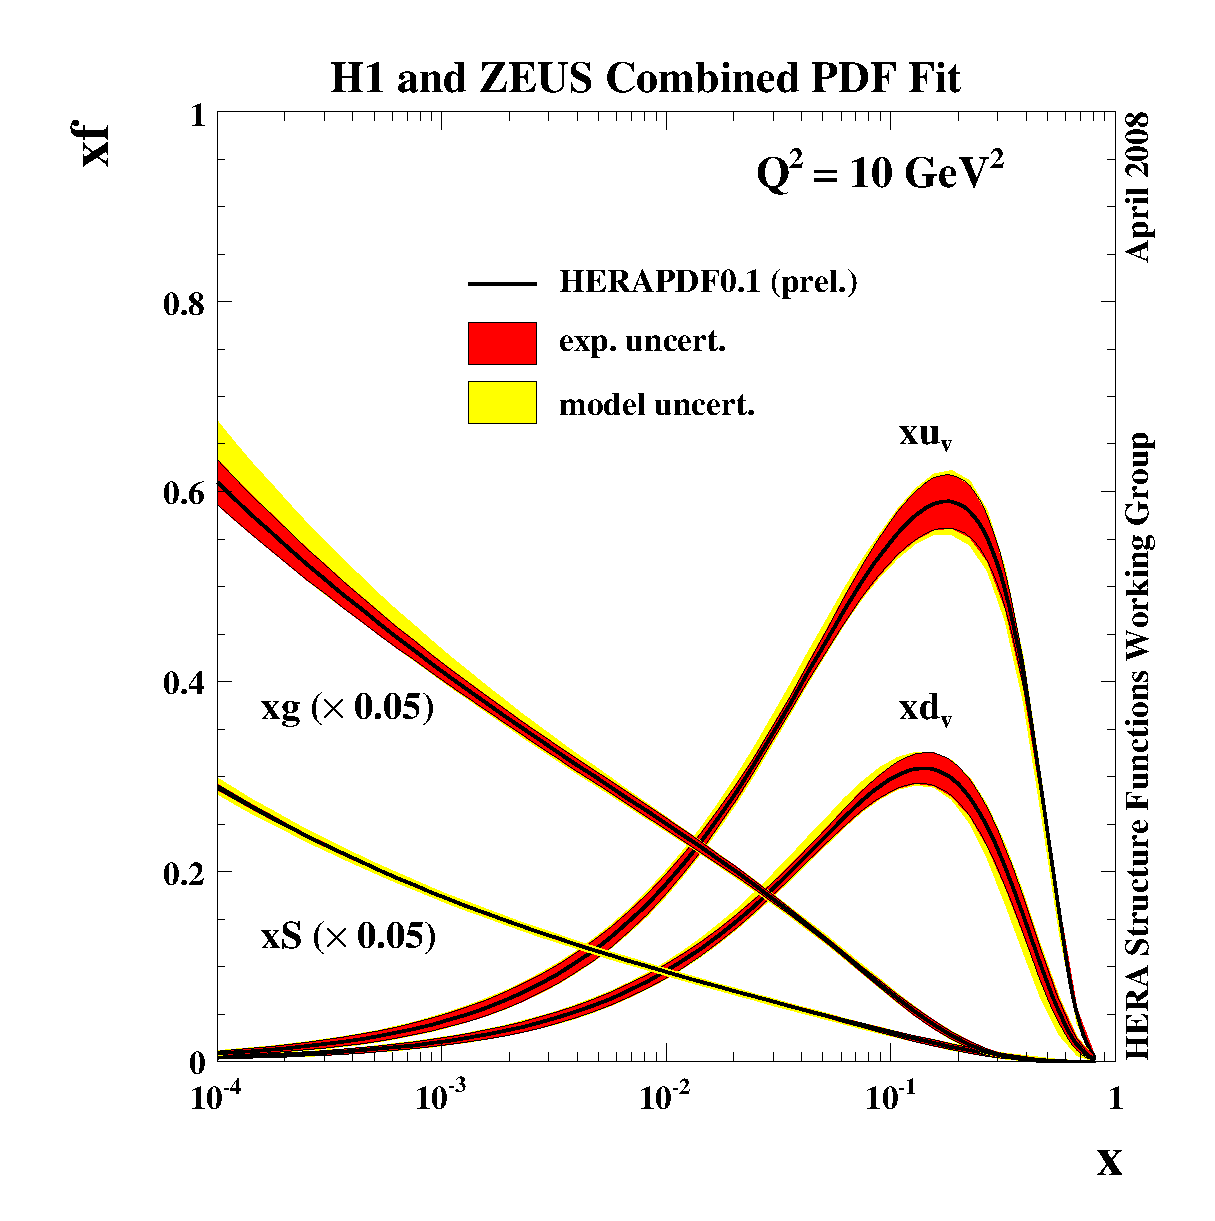
\includegraphics[width=0.4\textwidth]{\imgpath/pdf.eps}
\caption{Parton distribution functions determined at HERA. TBA}
\label{fig:intro:pdfs}
\end{figure}

\subsection{Parton fragmentation and the Lund string}

After the scattering process, the produced partons continue to fragment by emitting more partons in a process called the parton shower. Since the coupling strength in QCD increases with decreasing the energy scale of the splitting, this leads to the production of many soft, collimated emissions known as jets. The partonic evolution continues until the virtuality of the partons reaches the hadronization scale ($\approx \Lambda_\mathrm{QCD}$). There are multiple frameworks within QCD to describe the evolution of partons into their final state, such as using the DGLAP equations or the so-called dipole formalism.

Once the partonic final state is reached, the partons hadronise into the observable mesons and baryons. The hadronisation process is not calculable in QCD and requires phenomenological models to describe it. One such model is the Lund String model, which describes hadronisation as the breaking of a color string between the quarks in the final state. In this model, the energy stored in the color string is converted into the mass of new hadrons.

According to confinement, hadronisation should involve at least two partons with complementary colours. In QCD, the $q\bar{q}$ potential takes the shape of
\begin{align}
V_{q\bar{q}} \approx - \frac{4}{3}\frac{\alpha_s \hbar c}{r} + \kappa r \quad ,
\end{align}
where $\kappa$ is a paramater with value around $1 \mathrm{GeV} /\mathrm{fm}$. In the non-perturbative regime (long distances), the potential is dominated by the linear part, which is reminiscent of a system bound by a string with tension $\kappa$. This is taken advantage of by the Lund string model -- a $q$ and $\bar{q}$ pair separated by distance $\Delta x$ is bound by a color field (string) with energy $\kappa \Delta x$. 

If the $q$ and $\bar{q}$ continue separating as a result of the scattering, the energy stored in the color field increases. At some point, it can become energetically favourable to produce a new $q\bar{q}$ pair out of vacuum, which is a quantum mechanics tunnelling phenomenon characterised by the probability:
\begin{align}
\frac{\mathrm{d}P}{\mathrm{d}m_\mathrm{T}} \propto \exp \left( -\frac{\pi m_\mathrm{T}^2}{\kappa} \right) \quad ,
\label{eq:intro:tunnel}
\end{align}
where $m_\mathrm{T}$ is the transverse mass of the produced quarks. Otherwise, the $q\bar{q}$ system starts contracting and oscillates with a period $T = 2 E_\mathrm{kin}/\kappa$, where $E_\mathrm{kin}$ is its maximum kinetic energy. The produced $q$ and $\bar{q}$ then connect by new color fields to the original pair. This process repeats itself result in cascade of many $q\bar{q}$ pair connected by many color strings. In this descriptions, baryons can also be created by double tunnelling of a $qq\bar{qq}$ pair. The process is illustrated in Fig.~\ref{eq:intro:lundstring}.

\begin{figure}[H]
\subfloat[][]{\includegraphics[width=.330\textwidth]{\imgpath/tubelike.png}}
\subfloat[][]{\includegraphics[width=.330\textwidth]{\imgpath/lundstring.png}}
\subfloat[][]{\includegraphics[width=.330\textwidth]{\imgpath/lundgluon.png}}
\caption{Illustration of the color field between two quarks and its simplified representation with a string. Illustration of the string splitting by producing new $q\bar{q}$ in the $t-z$ plane. Illustration of the treatment of gluons in the Lund string model.}
\label{fig:intro:lundstring}
\end{figure}

Equation \ref{eq:intro:tunnel} also implies that production of strange quarks is suppressed by a factor of 
\begin{align}
\rho = \exp \left( -\frac{\pi (m^2_s - m^2_{u,d})}{\kappa} \right) \quad .
\end{align}
This parameter is typically tuned to data, as substituting constituent ($m_s \approx \gevcc{0.5}$, $m_{u,d} \approx \gevcc{0.33}$) versus current masses ($m_s \approx \gevcc{0.1}$, $m_{u,d} \approx 0$) leads to considerable differences underestimating and overestimating data, respectively.

For a $q\bar{q}g$ system, in this model, the gluon connects to the quark and antiquark and is effectively treated as a ``kink" on the color field, adding energy and momentum to the $q\bar{q}$ string (stretching it in its direction), as visualised in Fig.~\ref{eq:intro:lundstring}.

It should be noted that in the paradigm of AA collisions, hadron production can be alternatively modelled by hadronisation at the QGP's phase boundary by \textit{coalescing} free quarks.
%CooperFrye freezeout

%%!!!!TBA a sentence about the actual hadronisation.

\section{Multiple partonic interactions}

Results from $\mathrm{Sp\bar{p}S}$ in the 1980s sparked motivations for considering interactions of multiple partons between the two composite protons. For example, the AFS experiment observed an abundance of 4-jet events, displayed in Fig.~\ref{fig:intro:afs4jet}, that could not be explained by calculations considering a double gluon bremststrahlung from a single partonic scattering\cite{afs-4jet}. Furthermore, UA5 measurements studying energy dependence of multiplicity distributions P(\Nch) from  revealed a significant broadening when increasing $\sqrt{s}$, and saw the so-called KNO scaling\cite{kno-scaling}, where P(\Nch)/\meanNch remains constant, which was not reproducible in the context of \Nch being produced from a single string\cite{ua5-broadening}. This further suggested at the presence of multiple production sources.

\begin{figure}[H]
\subfloat[][]{\includegraphics[width=.520\textwidth]{\imgpath/afs4jet.png}} 
\subfloat[][]{\includegraphics[width=.380\textwidth]{\imgpath/sigmampi.pdf}}
\caption{TBA.}
\label{fig:intro:afs4jet}
\end{figure}

These findings prompted further development of Regge theory and approaches that incorporated multiple pomerons, which were successful in describing the \Nch distributions. However, this approach is fully decoupled from descriptions of the perturbative primary scattering. Subsequently, much of the phenomenology related to multiple partonic interactions was developed within the framework of the Pythia MC event generator, which is discussed individually in Section X. However, nowadays, the relevance of the concept of MPIs in hadronic collisions extends beyond this generator. A scattering with double partonic interactions is illustrated in Fig.~\ref{fig:intro:dps}.

\begin{figure}[H]
\includegraphics[height=7em]{\imgpath/dps.png}
\caption{TBA.}
\label{fig:intro:dps}
\end{figure}

In the Pythia approach, MPI are treated as additional perturbative scatterings. In QCD, the $2\to2$ cross section (dominated by the gluon exchange t-channel) diverges as $\propto \alpha^2_S(k_{\perp}^2)/k_{\perp}^4$, so a cutoff parameter $k_{\perp/\mathrm{min}}$ must be introduced, and using (\ref{fig:intro:factorization}) leads to:
\begin{align}
\frac{d\sigma}{dk_{\perp}^2} &= \sum_{ij}\int dx_1 dx_2 f_i(x_1,\mu_F^2)f_j(x_2,\mu_F^2) \frac{d\hat{\sigma}^H_{ij}}{dk_{\perp}^2} \, , \\
\sigma_{\text{int}}(k_{\perp\text{min}}) &= \int_{k_{\perp\text{min}}^2}^{s/4} \frac{d\sigma}{dk_{\perp}^2}dk_{\perp}^2 \, .
\end{align}
The choice of cutoff can be tuned to experimental data, and for the $\mathrm{Sp\bar{p}S}$ energy of \sppg{630}, a value of around \gevc{1.6} was typical. The dependence of this parton-parton scattering cross section is shown in Fig.~\ref{fig:intro:afs4jet}.

The total pp cross-section is given by
\begin{align}
\sigma_{\mathrm{pp}} &= \sigma_{\mathrm{elastic}} + \sigma_{\mathrm{single \, dif.}} + \sigma_{\mathrm{double \, dif.}} + \sigma_{\mathrm{non-dif.}} \quad , 
\end{align}
where the inelastic cross sections corresponds to approximately 60\% of the total. The mean number of MPIs, \meannmpi, can be estimated using:
\begin{align}
\meannmpi (k_{\perp,\mathrm{min}}) = \frac{\sigma_{\mathrm{int}}(k_{\perp,\mathrm{min}})}{\sigma_{\mathrm{inel}}}
\end{align}

However, the actual treatment is more complex and involves considerations of other parameters such as $k_\perp^0$ to account for the confinement nature of partons, modifications of multiparton PDFs, energy-momentum conservation, and the intertwinedness of partonic evolutions.



In summary, MPIs represent several subcollisions that take place in an average pp collision with \pt scales of a few GeV. They are colour-connected to the beam remnants, which in the Lund model are represented by strings. Since a string with $\kappa = 1 \mathrm{GeV} /\mathrm{fm}$ yields, as a rule of thumb, approximately one hadron per unit rapidity, and the average pp collision at the LHC at \sppt{13} has $\langle \dndy \rangle \approx 6$, the typical number of partonic interactions is around six.

Finally, the observation of QGP-like phenomena in pp collisions at the LHC has renewed interest in MPI phenomenology, as discussed in the following chapter. Such observations do not contradict the concept of MPIs; rather, they suggest the possibility of incorporating collective behavior among the MPIs, such as interactions between strings, local modifications of string tensions, or, alternatively, the formation of a multipartonic state with QGP-like properties.

\subsection{Color reconnection}

The incorporation of MPIs improved the description of the \Nch distributions and their dependence on $\sqrt{n}$. However, there were also observations of $\meanpt(\Nch)$ increasing as a function of \Nch, which could not be explained. More MPIs lead to more strings, which in turn leads to the production of more particles, but the \pt is mostly unaffected. This would predict a weaker dependence of \meanpt on \Nch, contrary to the data. The issue was resolved by implementing a possible color reconnection mechanism, which rearranges the color fields between partons.

TBA Insert diagrams of the processes!

One can envision the following process:
\begin{align*}
e^+ e^- \rightarrow W^+ W^- \rightarrow q_1\bar{q}_2 q_3\bar{q}_4  .
\end{align*}
In this scenario, a color reconnection mechanism could rearrange the colour-connected $q_1\bar{q}_2$ and $q_3\bar{q}_4$ into $q_1\bar{q}_4$ and $q_3\bar{q}_2$ if it were energetically favourable, depending on the phase-space configurations. Measurements at LEP of this process have indeed shown that such final-state corrections must be taken into account to explain the data on $W$ masses and widths. They also reported that the reconnection probabilities for such events are on the order of $50\%$, further indicating that colour reconnection is an important factor to consider.

Pythia implements CR by minimizing the total length of strings in the system, analogous to minimising potential energy. This mechanism, illustrated in Fig.~\ref{fig:intro:cr}, explains the rising trend of $\meanpt(\Nch)$: shorter strings imply fewer hadrons to split the transverse boost across, and the more MPI, the bigger this effect. Moreover, CR also helped describe the absolute value of \meanpt. With this approach, no further modifications of fragmentation parameters were necessary, in line with the concept of jet universality. However, it should be noted that there are various CR implementations and all rely on parameters obtained from tuning to data.

\begin{figure}[H]
\includegraphics[height=7em]{\imgpath/cr.png}
\caption{a) In a hard parton subcollision, the outgoing gluons are connected to the beam remnants through colour. Additional gluon kinks may occur through initial state radiation, which are ordered by rapidity. (b) A second hard scattering should theoretically result in two new strings connected to the remnants. (c) In order to minimise the total string length, gluons are colour reconnected.}
\label{fig:intro:cr}
\end{figure}

It is also worth noting that the \pt boost acquired through color reconnection may depend on mass and whether a hadron is a baryon or meson, which somewhat mimics the hydrodynamic signatures of collective flow observed in AA collisions.

\section{Underlying event}

The underlying event (UE) in high-energy collisions refers to the additional hadronic activity that accompanies the primary hard scattering process, but is not directly related to it. This includes the fragmentation products of the beam remnants, ISR and FSR, as well as the effects of the previously discussed MPIs. The UE is typically characterized by the distribution of softer particles around and far outside of the hard process.

It is important to note that the UE is different from the MB production, as it is biased by the presence of hard scattering. Additionally, the magnitude of the UE can fluctuate from event to event.

TBA Maybe some illustration/plot

\section{Lattice QCD}

One paragraph

\section{QCD phase diagram}

One paragraph, figure

\subsection{Phase transition}

One paragraph, bag model derivation of $T$

\subsection{Chiral symmetry restoration}

One paragraph, figure

\section{Implications of high-activity QCD research}

One paragraph
\chapter{QCD phenomena in high energy hadronic collisions}
\def \imgpath {"./figures/colls"}

The aim of this chapter is to give an introduction to the physics of heavy ions and the various phenomena related with the quark-gluon plasma QGP. Furthermore, a detailed summary of the findings of QGP phenomena in small systems, i.e.\ pp and pA collisions, is given. Lastly, some Monte Carlo event generators based on phenomenological modelling of hadronic collisions relevant to this dissertation are summarised.

\section{Collisions of heavy nuclei}

\subsection{Collision geometry, centrality, multiplicity}

Collisions of heavy nuclei, composed of many fluctuating nucleons, may occur under various initial state configurations. Some quantities used to describe them are the impact parameter $b$, defined as the distance between the two nuclei centers, number of participating (scattered) nucleons $\Npart$, and the number of binary nucleonic collisions $\Ncoll$.

Determining these quantities is important because:
\begin{enumerate}
\item Soft processes, such as light flavor particle production, are expected to scale with the interaction volume, which $\propto \Npart$.
\item Hard processes, such as jet and heavy flavor production, are expected to scale with the number of large momentum transfer interactions given by \Ncoll.
\item $b$, disregarding the fluctuations of nucleonic positions, defines the shape and anisotropy of the overlap region, which are important initial state conditions.
\end{enumerate}

Since these quantities cannot be directly measured, they need to be modelled. The charged particle \textit{multiplicity} is commonly used for this purpose, as \meanNch increases monotonically with \Npart, \Ncoll, and decreasing $b$. Multiplicity \Nch can be measured experimentally, e.g.\ with tracking detectors. The concept of \textit{centrality} is also used, which is defined as quantiles of the total nuclear cross-section. For example, a centrality of $0-5\%$ refers to low $b$ values and the top $5\%$ of \Nch values (central events), while $95-100\%$ centrality refers to high $b$ values and the bottom $5\%$ of \Nch values (peripheral events). Centrality can also be inferred from other \textit{event activity} classifiers, such as amplitudes of scintillators at forward rapidity, transverse energy in calorimeters, or energy from beam remnants in zero-degree-calorimeters.

In AA collisions, these relationships are well-defined, and thus the models perform well. The most popular model is the MC Glauber model \cite{millerGlauberModelingHigh2007}. Other models include MC-KLN \cite{kharzeevHadronProductionNuclear2001} and IP Glasma \cite{schenkeFluctuatingGlasmaInitial2012}.

\subsection{MC Glauber model}

The MC Glauber model \cite{millerGlauberModelingHigh2007} takes on a very simple albeit powerful approach. The two nuclei are simulated in three dimensions in a way that satisfies their respective nuclear density profiles, usually modelled by sampling the positions of nucleons from the Woods-Saxon distribution:

\begin{minipage}{0.4\linewidth}
    \begin{center}
        \begin{tikzpicture}
            \draw[->] (-0.25,0) -- (2.5,0) node[right] {$r$};
            \draw[->] (0,-0.2) -- (0,1.2) node[above] {$n(r)$};
            \draw[scale=1,domain=-0.15:2.2,smooth,variable=\x,blue] plot ({\x},{1/(1+exp((\x-1.5)/0.1))});
            \draw[dashed] (1.5,0) node[below] {$R$} -- (1.5,1);
        \end{tikzpicture}
    \end{center}
\end{minipage}%
\begin{minipage}{0.6\linewidth}
    \begin{equation}
        n(r) = \frac{1}{1+\exp((r-R)/a)} \quad ,
    \end{equation}
\end{minipage}

where $R$ is the nuclear radius and $a$ the nuclear skin thickness.

The nucleonic densities can be represented by uniform disks, or more accurately by Fermi-distributions or Gaussian profiles to account for fluctuations of their densities. Their parameters are left free and are tuned to the data.

A random impact parameter is then chosen or sampled. The collision is then treated as a sequence of independent binary nucleon-nucleon collisions, where
\begin{enumerate}
\item nucleons remain travelling in straight lines,
\item the inelastic nucleon-nucleon cross section $\sigma_\mathrm{NN}$ does not depend on the number of interactions,
\item two nucleons are considered to interact if their transverse relative distance $d \leq \sqrt{\sigma_\mathrm{NN}/\pi}$.
\end{enumerate}

Figure~\ref{fig:colls:centrality} illustrates an example of a Glauber Monte Carlo event for a Au+Au collision. By simulating numerous collisions, the average \Npart and \Ncoll are determined\footnote{It also shows the scaling between the numbers of participants and binary collisions, which is approximately $\Ncoll \approx 0.35 \Npart^{4/3}$ .}, and their relations to centrality and event activity observables are determined by fitting to experimental data.

Recent studies have extended the MC Glauber model to include sub-nucleonic structures. Such efforts show that the production of charged hadrons at mid-rapidity scales linearly with the number of participating partons. Comparisons with LHC data at \snnt{5.02} suggest that the number of sub-nucleonic degrees of freedom ranges from $3$ to $5$ \cite{loizidesGlauberModelingHighenergy2016}.

\begin{figure}[H]
\subfloat[][]{\adjustbox{valign=m}{\adjincludegraphics[trim={{.33\width} 0 {.33\width} 0},clip,width=.29\textwidth]{\imgpath/glauber_mc_event.pdf}}}\hspace{2em}
\subfloat[][]{\adjustbox{valign=m}{\includegraphics[width=.490\textwidth]{\imgpath/cocktail3.eps}}}
\caption{\textbf{(a)} Glauber Monte Carlo event of a Au+Au collision at \snng{200} shown in the transverse plane (top panel) and along the beam axis $z$ (bottom panel). The darker circles represent participating nuclei and their area corresponds to $\sigma_\mathrm{NN}$. \textbf{(b)} Illustrative diagram of the dependence of final-state event multiplicity on the initial-state quantities, number of participants \Npart and impact parameter $b$. \cite{millerGlauberModelingHigh2007}}
\label{fig:colls:centrality}
\end{figure}

\section{Quark-gluon plasma}

In agreement with lattice QCD predictions \cite{borsanyiThermodynamicsQCDTransition2013}, the QGP has been measured in ultra-relativistic collisions of heavy nuclei at RHIC \cite{arseneQuarkGluonPlasma2005, adamsExperimentalTheoreticalChallenges2005}, LHC \cite{niidaSignaturesQGPRHIC2021}, and even SPS \cite{heinzEvidenceNewState2000}. Although it cannot be observed directly, a wealth of evidence from three decades of research combining various observables reveals the effects of the produced QGP medium. Whilst somewhat context-dependent, the following features make QGP the most extreme phenomenon observed in terms of its:
\begin{itemize}
\item \textit{Temperature}: QGP temperatures reach values on the order of hundreds of MeV, which corresponds to approximately $2 \times 10^{12}$~K.\footnote{Contrasting some of the lowest temperatures required for the super-conducting magnets of the LHC, $T \approx 1.9$~K.} \cite{cmscollaborationMeasurementNuclearModification2019}
\item \textit{Viscosity}: the shear viscosity to entropy density ratio $\eta/s$ reaches the minimum quantum limit of $1/4\pi$ (for water at room temperature, $\eta/s \approx 8$), making it an almost perfect liquid. \cite{pasechnikPhenomenologicalReviewQuark2017}
\item \textit{Vorticity}: in semi-peripheral collisions, the rotating plasma reaches a vorticity of approximately $9\times 10^{21}$ s$^{-1}$. \cite{adamczykGlobalHyperonPolarization2017}
\item \textit{Magnetic field}: in non-central collisions, the magnetic fields in the system may peak at $\sim 10^{19}$ T. \cite{kharzeevEffectsTopologicalCharge2008}
\end{itemize}

\begin{figure}[H]
\includegraphics[width=.90\textwidth]{\imgpath/evolution.pdf}\\
\caption{Evolution of heavy nuclei collisions at LHC energies, depicting the different stages. \cite{alicecollaborationALICEExperimentJourney2022}}
\label{fig:colls:evolution}
\end{figure}

Figure~\ref{fig:colls:evolution} illustrates the common paradigm for the different stages of a collision between heavy nuclei:
\begin{enumerate}
\item The Lorentz-contracted heavy nuclei approach each other at ultra-relativistic speeds.
\item \textit{Pre-hydrodynamisation stage} ($\tau \equiv \sqrt{t^2 - z^2} \leq 1$ fm/c): ``hard" particles are produced in scatterings with the highest momentum transfer $Q^2$. Produced matter expands rapidly in the longitudinal direction and starts expanding in the radial direction.
\item \textit{Hydrodynamisation} ($1 \leq \tau \leq 10$ fm/c): abundantly produced partons create a deconfined medium, which can be described by hydrodynamic equations.
\item \textit{Chemical freeze-out} ($\tau \sim 10$ fm/c): the system cools down and hadronises. The produced hadrons then stop interacting inelastically and the system's chemical content is stabilised.
\item \textit{Kinetic freeze-out} ($\tau \lesssim 20$ fm/c): hadrons no longer interact elastically and their kinematics stabilize.
\item Long-lived particles can be measured in the detector volume. 
\end{enumerate}

The following subsections outline some of the essential phenomena related to the production of QGP.

\subsection{Quarkonium dissociation and sequential suppression}

Heavy quarkonia are vector meson states consisting of $c\bar{c}$ and $b\bar{b}$. They include $J/\psi$, $\psi(2\mathrm{S})$, $\Upsilon(1\mathrm{S})$, $\Upsilon(2\mathrm{S})$, $\Upsilon(3\mathrm{S})$, which can be relatively easily measured in LHC experiments via their di-lepton decay channels. They are created solely in the first phases of the collision and then experience the entire evolution of the QGP medium:
\begin{equation}
t^{Q\overline{Q}}_\mathrm{creation} < t^\mathrm{QGP}_\mathrm{creation} < t^\mathrm{QGP}_\mathrm{lifetime} \ll t^{Q\overline{Q}}_\mathrm{lifetime} \quad .
\end{equation}

Additionally, due to their large binding energies, their radii may remain smaller than the plasma screening radius $r_\mathrm{D}(T)$, and thus, survive the dissociation. For instance, considering their in-vacuum radii determined from the $q\bar{q}$ potential, $r_{\Upsilon(1\mathrm{S})}\sim 0.14$~fm, $r_{\Upsilon(2\mathrm{S})}\sim 0.28$~fm, $r_{\Upsilon(3\mathrm{S})}\sim 0.39$~fm, which contrast the $r_\pi \sim 0.7$~fm \cite{sarkarPhysicsQuarkGluonPlasma2010}. This implies that different temperatures result in the dissociation of different states, and measuring the production of different states can help infer the QGP temperature, as illustrated in Fig.~\ref{fig:colls:thermometer} \cite{matsuiSuppressionQuarkgluonPlasma1986, satzProbingStatesMatter2013}.

\begin{figure}[H]
\includegraphics[width=.70\textwidth]{\imgpath/spec.eps}
\caption{Spectral lines corresponding to various charmonium and bottomonium states for different medium temperatures , relative to the QGP critical temperature. \cite{satzProbingStatesMatter2013}}
\label{fig:colls:thermometer}
\end{figure}

The production of heavy quarkonia in AA collisions is compared to that in pp collisions (scaled by the average number of binary collisions) through the nuclear modification factor, $R_{\mathrm{AA}}$. This quantity is widely used in various other measurements and is defined as:
\begin{align}
R_{\mathrm{AA}}=\frac{\mathrm{d}N_{\mathrm{AA}}/\mathrm{d}\pt}{\langle N_{\mathrm{coll}}\rangle\ \mathrm{d}N_{\mathrm{pp}}/\mathrm{d}\pt} \quad .
\end{align}
$R_{\mathrm{AA}}$ can take on the following values:
\begin{enumerate}
\item $R_\mathrm{AA} = 1$: The result one would expect if the AA collision is a mere superposition of nucleon-nucleon collisions. There is no net effect on the production, corresponding to the absence of the QGP medium and other nuclear effects, or their mutual cancellation.
\item $R_\mathrm{AA} < 1$: The production is overall suppressed, for example, due to dissociation.
\item $R_\mathrm{AA} > 1$: The plasma and nuclear effects systematically enhance the measured production.
\end{enumerate}

At LHC energies, the abundance of charm quarks in the QGP is high enough that charmonia can be formed after dissociation, which somewhat complicates the interpretation of charmonia suppression. However, the $\Upsilon(3\mathrm{S})$ bottomonium has $R_{\mathrm{AA}}$ consistent with zero at $\sqrt{s_{\mathrm{NN}}}=5.02$ TeV, as shown in Fig.~\ref{fig:colls:cmsupsilon} \cite{cmscollaborationMeasurementNuclearModification2019}. This complete suppression is a clear signature of the QGP and can be used together with models to estimate the QGP temperature at these energies as $T\approx 630$~MeV \cite{krouppaPredictionsBottomoniaSuppression2016}.

\begin{figure}[H]
\subfloat[][]{\includegraphics[width=.40\textwidth]{\imgpath/cms_ups1.pdf}}\hspace{2em} 
\subfloat[][]{\includegraphics[width=.41\textwidth]{\imgpath/cms_ups2.pdf}}
\caption{\textbf{(a)} Muon invariant mass distributions in Pb-Pb collisions at \snnt{5.02}, also showing a scaled result from pp collisions at same energies (red dashed line). \textbf{(b)} Nuclear modification factors of the three bottomonium states. \cite{cmscollaborationMeasurementNuclearModification2019}}
\label{fig:colls:cmsupsilon}
\end{figure}

\subsection{Strangeness enhancement}

In the production of hadrons in vacuum, strangeness is suppressed relatively to light quarks not only due to the higher mass of the strange quark ($m_s \approx \gevcc{0.1}$), but also due to the much higher constituent mass ($m_K \approx \gevcc{0.5}$). However, in the QGP, due to the high gluon densities and $T\sim m_s$, strangeness production may equilibrate with $u$ and $d$ quarks through gluon fusion:
\begin{align*}
gg \to s\bar{s} \quad .
\end{align*}

This phenomenon was proposed as one of the first signatures of QGP observation in colliders \cite{rafelskiStrangenessProductionQuarkGluon1982, kochStrangenessRelativisticHeavy1986}. Indeed, an enhancement in the production of strange hadrons is observed in AA collisions, which is dependent on the event activity and increases with increasing strangeness content of the hadron \cite{alicecollaborationMultistrangeBaryonProduction2016}. Figure~\ref{fig:colls:strangeness} displays these results.

Furthermore, the yields of hadrons measured in AA collisions can be accurately described by statistical models \cite{andronicThermalHadronProduction2009, wheatonTHERMUSThermalModel2009} which, generally, assume that the dense system is in thermal and chemical equilibrium at the point of its freeze-out. In these models, strangeness is assumed to be conserved on average, which corresponds to a grand-canonical ensemble with a strange chemical potential $\mu_S$. 

In small systems, the conservation of strangeness must be taken into account for each interaction, locally. This necessitates the use of a canonical ensemble and introducing a parameter, $V_0$, to describe the volume of this locality requirement \cite{hamiehCanonicalDescriptionStrangeness2000}. With this approach, strangeness enhancement can be reproduced by increasing $V_0$ and transitioning from the canonical ensemble in small systems to the grand-canonical ensemble in AA collisions, as depicted in Fig.~\ref{fig:colls:strangeness}.

\begin{figure}[H]
\subfloat[][]{\includegraphics[height=11.85em]{\imgpath/se_v02.pdf}}\hspace{1em}
\subfloat[][]{\includegraphics[height=13em]{\imgpath/se_omegaxi.pdf}}
\caption{\textbf{(a)} Dependence of strange baryon densities on the parameter $V_0$ characterising the volume where strangeness is locally conserved in models describing strangeness suppression in small systems as canonical suppression. The volume is normalised to a typical AA value of $\overline{V}_0=7.4$~fm$^{3}$. \cite{hamiehCanonicalDescriptionStrangeness2000}. \textbf{(b)} Ratios of yields of strange baryons to pions in pp, p-Pb, and Pb-Pb collisions as a function of the pion multiplicity normalised to the high-multiplicity limit in $0-60\%$ most central Pb-Pb collisions. The results are compared with a statistical model combining the canonical and grand-canonical approach. \cite{alicecollaborationMultistrangeBaryonProduction2016, wheatonTHERMUSThermalModel2009}}
\label{fig:colls:strangeness}
\end{figure}

%\begin{figure}[H]
%\subfloat[][]{\includegraphics[width=.47\textwidth]{\imgpath/xitopi.pdf}}\hspace{1em}
%\subfloat[][]{\includegraphics[width=.47\textwidth]{\imgpath/omegatopi.pdf}}
%\caption{TBA}
%\label{fig:colls:strangeness}
%\end{figure}

\subsection{Collective flow}

The strongly interacting plasma exhibits a collective expansion which can be described by hydrodynamic equations, since the mean free paths of the constituents are much smaller than the system size ($\lambda \ll L$). The non-uniform energy density in the initial state results in varying pressure gradients, which drive this expansion. Since the centre of the plasma has greater pressure than its outside regions, common expansion velocity field develops, which results in the so-called \textit{radial flow}. Similarly, the medium also translates the directionally-dependent anisotropies in the initial state, which stem from the almond-shape geometry of the collision overlap region as well as nucleonic fluctuations, to the final-state. This is the so-called \textit{anisotropic flow}.

Together with hadronic re-scattering, the flows are reflected in the kinematics of the final-state hadrons. When comparing \pt spectra in central AA collisions to those in peripheral or in pp collisions, a broadening as well as a momentum boost can be observed (see Fig.~\ref{fig:colls:rflow}), caused by the radial expansion as well as the less important thermal motion \cite{alicecollaborationCentralityDependenceRm2013, alicecollaborationRmSRm2013, alicecollaboration8920Phi2015}. The expansion effect depends on the mass of the hadrons, as the amount of additional \pt acquired is proportional to their mass and the collective expansion velocity field, $p \approx m\beta c$. A notable exception to this trend is the $\phi$ quarkonium; although comparable with the proton ($m_\phi \approx \gevcc{1.02} \sim m_p$), its scattering cross-section is much smaller \cite{hungEquationStateRadial1998}.

The \pt spectra influenced by radial flow can be described by the Blast-Wave parametrisation \cite{schnedermannThermalPhenomenologyHadrons1993}. In this approach, the radial expansion is accounted for as a common velocity field profile $\beta (r)$ affecting thermal spectra, 

\begin{minipage}{0.5\linewidth}
    \begin{center}
        \begin{tikzpicture}
            \draw[->] (-0.25,0) -- (2.5,0) node[right] {$r$};
            \draw[->] (0,-0.2) -- (0,1.2) node[above] {$\beta(r)$};
            \draw[scale=1,domain=0.0:2.2,smooth,variable=\x,blue] plot ({\x},{0.95*(\x/2.2)^0.7});
            \draw[dashed] (2.2,0) node[below] {$R$} -- (2.2,1);
        \end{tikzpicture}
    \end{center}
\end{minipage}%
\begin{minipage}{0.5\linewidth}
    \begin{equation}
		\beta (r) = \beta_s (\frac{r}{R})^n \quad ,
    \end{equation}
\end{minipage}

where $\beta_s$, $R$, and $n$ are the expansion velocity on the surface of the plasma, its radius, and an extra parameter usually ranging $0.7-1.0$ in central collisions \cite{alicecollaborationCentralityDependenceRm2013}, respectively. The effects of radial flow can also be reproduced in AA collisions with hydrodynamic models using an equation of state from LQCD and hadronic re-scattering \cite{hungEquationStateRadial1998}, and in pA collisions with the EPOS3 model, which also incorporates hydrodynamic evolution in QGP droplets \cite{wernerAnalysingRadialFlow2014}.

Ratios of baryons to mesons, such as $p/\pi$ or \ltok, as a function of event activity are often used to demonstrate the effect of radial flow, as shown in Fig.~\ref{fig:colls:rflow}. In these ratios, the modification of \pt spectra results in the following effects on the high-event-activity ratios:
\begin{enumerate}
\item The peak in the ratio is shifted to higher \pt by up to $\gevc{1.5}$,
\item there is an enhancement of baryons in the intermediate \pt $1.5 < \pt < \gevc{6}$ region,
\item and a corresponding depletion of baryons at low \pt.
\end{enumerate}

Figure~\ref{fig:colls:aflow} shows a typical shape of the initial state with its azimuthal anisotropy and the resulting pressure gradients. Anisotropic flow can be quantified by decomposing the azimuthal particle distribution into its Fourier series \cite{voloshinFlowStudyRelativistic1996}:
\begin{align}
\frac{dN}{d\varphi} \propto 1 + 2 \sum_{n=1}^{\infty} v_n e^{in(\varphi - \Psi_n)} \, , \quad \ v_n = \langle\cos[n(\phi - \Psi_n)]\rangle \, ,
\end{align}
where $\Psi_n$ is the symmetry plane of the $n$-th harmonic and $v_n$ is the Fourier coefficient corresponding to that harmonic, also known as the flow coefficient. In this context, a finite initial state ellipticity $\epsilon_2$ leads to a finite \textit{elliptic flow} $v_2$, triangularity $\epsilon_3$ to a \textit{triangular flow} $v_3$, and so on \cite{alverCollisionGeometryFluctuations2010, alicecollaborationHigherHarmonicAnisotropic2011}. 

\begin{figure}[H]
\subfloat[][]{\adjustbox{valign=m}{\includegraphics[width=.4\textwidth]{\imgpath/rfspectra.pdf}}}%\hspace{2em}
\subfloat[][]{\adjustbox{valign=m}{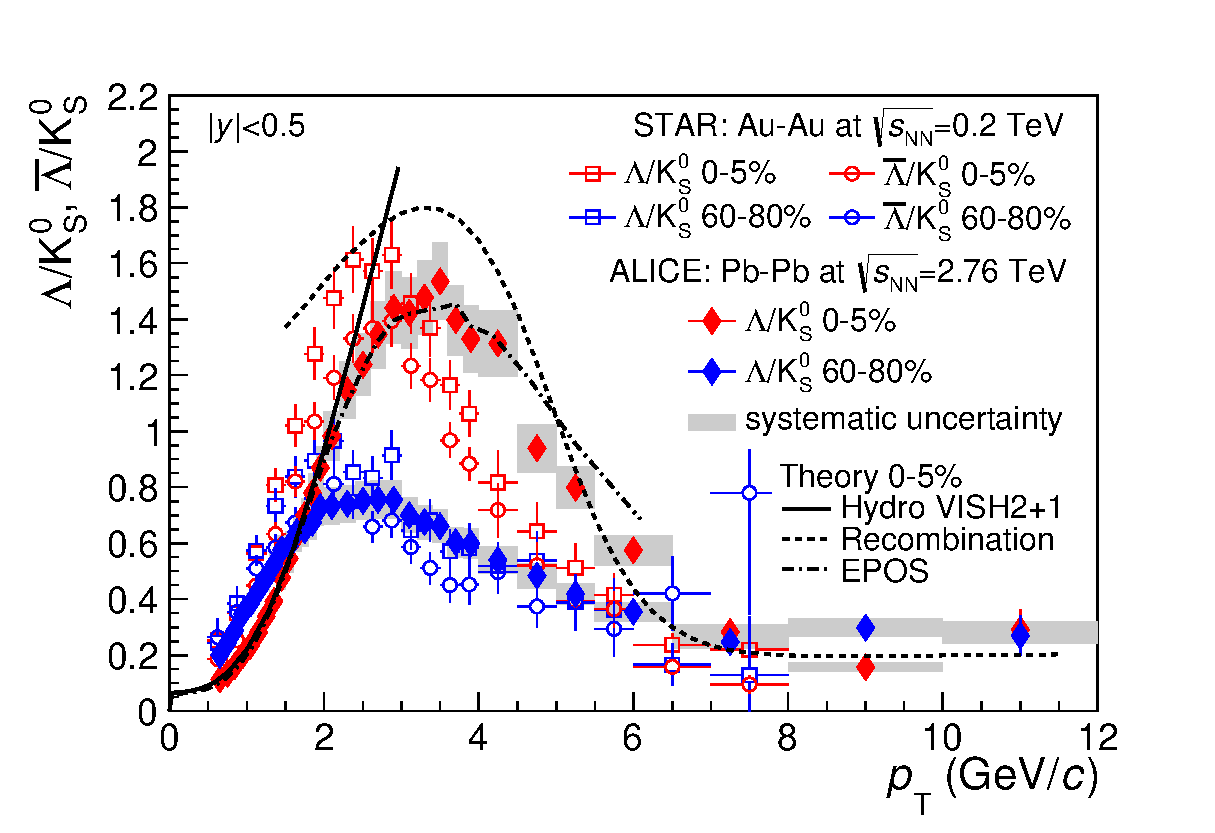
\includegraphics[width=.59\textwidth]{\imgpath/ltok.eps}}}
\caption{\textbf{(a)} Transverse momentum spectra of light-flavour hadrons in central $0-5\%$ and peripheral $80-90\%$ Pb-Pb collisions scaled by arbitrary factors to enhance the visibility. \cite{alicecollaborationALICEExperimentJourney2022, alicecollaborationCentralityDependenceRm2013, alicecollaborationRmSRm2013, alicecollaboration8920Phi2015} \textbf{(b)} \LA to \KOs ratios of transverse momentum spectra in Pb-Pb collisions at the LHC and Au-Au collisions at RHIC for central $0-5\%$ events (red) and peripheral $60-80\%$ events (blue). \cite{alicecollaborationRmSRm2013}}
\label{fig:colls:rflow}
\end{figure}

The flow coefficients can be experimentally extracted using various methods, including two-particle azimuthal correlations (as shown in Fig.~\ref{fig:colls:aflow}), and are typically studied as a function of event multiplicity. It is important to note that these azimuthal correlations between particles due to anisotropic flow are long-range, i.e.\ present consistently across the entire pseudorapidity range $\Delta \eta$ (the so-called ``ridge") \cite{luzumFlowFluctuationsLongrange2011}, which makes them distinguishable from similarly appearing ``non-flow" short-range correlations coming from jet fragmentation and resonance decays.
 
Moreover, measurements of $v_2$ in AA collisions for different particle species reveal a mass dependence in the low-\pt region, and a baryon/meson dependence in the intermediate \pt region, with baryons having approximately $1.5$ times higher values \cite{alicecollaborationEllipticFlowIdentified2015}. This suggests that the flow of hadrons is built up from its deconfined constituents.

\begin{figure}[H]
\subfloat[][]{\adjustbox{valign=m}{\includegraphics[width=.45\textwidth]{\imgpath/almond.png}}}\hspace{1em}
\subfloat[][]{\adjustbox{valign=m}{\includegraphics[width=.45\textwidth]{\imgpath/harmonics.pdf}}}
\caption{\textbf{(a)} Illustration of a collision of ultra-relativistic heavy nuclei and the overlapping region with pressure gradients (yellow). \cite{schadeApplicationsHolographyStrongly2012} \textbf{(b)} Correlation function of the relative azimuthal angle between a trigger particle and an associated particle, separated by a pseudorapidity gap, measured in central Pb-Pb collisions. The contributions from the elliptical, triangular, quadrupolar, and pentapolar harmonics are shown as different dashed lines. \cite{alicecollaborationHigherHarmonicAnisotropic2011}}
\label{fig:colls:aflow}
\end{figure}

\subsection{Jet quenching}

In AA collisions, partons produced in hard scattering processes interact with the colour charges in the quark-gluon plasma, resulting in the loss of energy through collisions and gluon bremstsstrahlung. This phenomenon is known as jet quenching and modifies or even "quenches" the parton shower \cite{gyulassyJetQuenchingDense1990, wangEffectJetQuenching1998}. In the factorisation theorem in Eq.~\ref{eq:intro:facto}, this corresponds to the medium-modification of the fragmentation functions. Studies of parton energy loss and jet quenching often use the transport coefficient $\hat{q}$, which describes the average \pt loss of a parton per a mean free path in the plasma and corresponds to the medium opacity

Jet quenching is one of the most important probes into the structure and dynamical properties of the QGP, since the hard partons experience its entire evolution, similarly to the case of heavy quarkonia discussed in Sec.~\ref{sec:colls:quarkonia}. It can also be compared with a large body of sound theoretical calculations \cite{gyulassyNonAbelianEnergyLoss2000} and MC simulations \cite{zappMonteCarloModel2009} based on QCD. Experimentally, jet quenching can manifest as suppression of the jet yield or even its complete disappearence, due to the energy loss of partons in the medium and their re-scattering. \cite{alicecollaborationALICEExperimentJourney2022}

Figure~\ref{fig:colls:jetquenching} displays such an AA event with a large jet imbalance and juxtaposes it with a pp event, where the leading and the recoil jet need to be balanced in azimuth due to conservation laws. Further effects and fields of study of jet quenching include the modification of jet substructures and shapes.

\begin{figure}[H]
\subfloat[][]{\includegraphics[height=11em]{\imgpath/DijetPP.pdf}}\hspace{2em} 
\subfloat[][]{\includegraphics[height=11em]{\imgpath/DijetAA.pdf}}
\caption{Event displays from CMS in azimuthal plane showing a collision of \textbf{(a)} pp and \textbf{(b)} Pb-Pb with a dijet. The red and blue columns correspond to energy deposits in the detector calorimeters. \cite{cmsCMSCollisionEvents2010, niidaSignaturesQGPRHIC2021}}
\label{fig:colls:jetquenching}
\end{figure}

\subsection{Cold nuclear matter effects}

It should be noted that apart from the QGP, other effects come into play due to the fact that the collision involves two nuclei instead of two protons. These effects are important caveats to bear in mind and include:

\begin{enumerate}
\item Nuclear (anti-)shadowing: Reflects the modification in production due to differences in nPDFs and PDFs. \cite{vogtShadowingEffectsPsi2015}
\item Cronin effect: Describes the initial parton energy loss due to scatterings in the nuclear medium and broadens measured \pt spectra. \cite{croninProductionHadronsLarge1975}
\item Nuclear absorption: Describes the dissociation of particles due to their interactions with the passing-by nuclear remnants \cite{wongIntroductionHighenergyHeavyion1990}. It is generally negligible at LHC energies.
\item Co-mover absorption: This is the effect of inelastic interactions with the hadron gas. \cite{ferreiroExcitedCharmoniumSuppression2015}
\end{enumerate}

These effects can be isolated and quantified in pA or very peripheral AA collisions.

\section{QGP phenomena in small systems}\label{sec:colls:qgpss}

Measurements within the last decade have shown that certain QGP phenomena can also be observed in high-multiplicity events of pp collisions at LHC energies, which challenges the traditional assumption that QGP is only produced in AA collisions. This has sparked debates about the existence of QGP in pp collisions and, to a lesser degree, about the absence of QGP in AA collisions, despite the extensive experimental evidence.

Furthermore, the observed behavior of these phenomena indicates that the role of event multiplicity \Nch may be more significant than the collision system size. This has led to ongoing efforts to establish a consistent and seamless link between the paradigms of pp and AA collisions.

\subsubsection*{Strangeness and charm enhancement}

ALICE measurements on $\LA/\pi$, $\XI/\pi$, and $\Omega/\pi$ ratios demonstrate that the production rates of particles containing strange quarks increase faster with multiplicity than those containing only u and d quarks \cite{adamEnhancedProductionMultistrange2017}. This also depends on the strangeness content -- the effect is the strongest for $\Omega$ and vanishes for protons. Furthermore, the evolution to larger systems seems to be continuous with respect to \Nch. The measurements can be seen in Fig.~\ref{fig:colls:ssstrangeness} \cite{alicecollaborationALICEExperimentJourney2022}.

To contrast the strangeness measurements with charm, the $J/\psi \ /\pi$ ratio also shows a clear increase in yield with increasing \Nch in pp collisions, as is shown in Fig.~\ref{fig:colls:ssstrangeness} \cite{alicecollaborationMultiplicityDependencePsi2020, alicecollaborationObservationMultiplicityDependence2022}. However, this comes with an important caveat: high-multiplicity events are biased to have enhanced hard processes, as discussed further in Chapter~\ref{chap:rt}. Moreover, the evolution of this phenomenon is also not continuous with \Nch when going from pp collisions at \sppt{13} to \snnt{5.02}, which can also be explained by the fact that charm quarks are produced solely in hard scattering processes, the rates of which depend on the collision system and center-of-mass energy.

\begin{figure}[H]
\subfloat[][]{\adjincludegraphics[trim={0 0 {.48\width} 0},clip,height=15em]{\imgpath/ss_strangeness1.pdf}}\hspace{2em}
\subfloat[][]{\adjincludegraphics[trim={0 0 {.948\width} 0},clip,height=15em]{\imgpath/ss_strangeness2.pdf}\adjincludegraphics[trim={{.52\width} 0 0 0},clip,height=15em]{\imgpath/ss_strangeness2.pdf}} 
\caption{Ratios of integrated yields of \textbf{(a)} various light-flavour hadrons \cite{adamEnhancedProductionMultistrange2017} and \textbf{(b)} charm mesons \cite{alicecollaborationMultiplicityDependencePsi2020, alicecollaborationObservationMultiplicityDependence2022} to pions as a function of multiplicity in pp, p-Pb, and Pb-Pb collisions. \cite{alicecollaborationALICEExperimentJourney2022}}
\label{fig:colls:ssstrangeness}
\end{figure}

\subsubsection*{Anisotropic flow}

Azimuthal correlations and anisotropic flow measurements in small collision systems exhibit features similar to those observed in AA collisions, hinting at the presence of collective expansion \cite{cmscollaborationEvidenceCollectivityPp2017}. However, in small systems, these measurements are particularly challenging due to their large sensitivity to non-flow effects, such as jet fragmentation or resonance decays, which can mimic the features of collective flow. 

While models using hydrodynamic-like descriptions seem to be able to describe $v_2$ results (despite the fact that their assumption $\lambda \ll L$ is not valid) \cite{wellerOneFluidRule2017}, especially at high multiplicities, the interpretation of the results in small systems is still under investigation. The values of elliptic flow $v_2$ seem to be comparable to those in low-multiplicity Pb-Pb collisions, although the evolution of $v_2$ across different system sizes does not appear to be smooth. The measurements from CMS displaying a clear ridge in high-multiplicity events \cite{cmscollaborationEvidenceCollectivityPp2017} and the $v_2$ results from ALICE \cite{alicecollaborationInvestigationsAnisotropicFlow2019} can be seen in Fig.~\ref{fig:colls:ssv2}.

\begin{figure}[H]
\subfloat[][]{\adjincludegraphics[trim={0 {0.67\height} 0 0},clip,width=0.45\textwidth]{\imgpath/ss_ridge1.pdf}}
\subfloat[][]{\adjincludegraphics[trim={0 {0.67\height} 0 0},clip,width=0.45\textwidth]{\imgpath/ss_ridge2.pdf}}\\
\adjincludegraphics[trim={0 {0.7\height} 0 0},clip,width=0.8\textwidth]{\imgpath/ss_v2.pdf}
\subfloat[][]{\adjincludegraphics[trim={0 0 0 {0.966\height}},clip,width=0.8\textwidth]{\imgpath/ss_v2.pdf}}
\caption{\textbf{(a, b)} Two-dimensional two-particle correlation functions of charged hadrons in low (left) and high (right) multiplicity events of pp collisions at \sppt{13}. \cite{cmscollaborationEvidenceCollectivityPp2017} \textbf{(c)} Elliptic flow measured using two-particle cumulants with a pseudorapidity separation in pp, p-Pb, Xe-Xe, and Pb-Pb collisions as a function of multiplicity. \cite{alicecollaborationInvestigationsAnisotropicFlow2019}}
\label{fig:colls:ssv2}
\end{figure}

\subsubsection*{Radial flow}

Measurements of the ratio of \LA to \KOs \pt spectra ratio were also studied in pp collisions with differing \Nch, see Fig.~\ref{fig:colls:ssrflow} \cite{alicecollaborationMultiplicityDependenceMulti2020}. The boost of a collectively expanding system, as expected in the context of radial flow, should have a greater impact on heavier hadrons, leading to an enhancement of the baryon-to-meson ratio at intermediate \pt. This enhancement is observed in the \LA/\KOs ratio, its magnitude increases with increasing \Nch and the peak position shifts towards higher values collisions, consistent with the hydrodynamic picture. The increase at intermediate momenta leads to a corresponding depletion at low \pt. High-\pt (as well as integrated) \LA/\KOs ratios exhibit essentially no (or minor) multiplicity dependence. This observation also applies to proton-to-pion ratios. 

Recent studies have also investigated the charmed baryon-to-meson ratio $\LA_c/\mathrm{D^0}$, with similar findings, although measurements with smaller uncertainties are still required. Fig.~\ref{fig:colls:ssrflow} presents the corresponding results.

\begin{figure}[H]
\includegraphics[width=.90\textwidth]{\imgpath/ss_rflow.pdf}
\caption{Baryon-to-meson ratios shown as the \pt differentials (left) and integrated yields in various \pt ranges as a function of multiplicity (right) for the \LA/\KOs and $\LA_c$/$\mathrm{D^0}$ in pp collisions at \sppt{13}. \cite{alicecollaborationMultiplicityDependenceMulti2020, alicecollaborationObservationMultiplicityDependence2022, alicecollaborationALICEExperimentJourney2022}}
\label{fig:colls:ssrflow}
\end{figure}

\subsubsection*{Sequential suppression of $\Upsilon$ states}

While defining $R_\mathrm{AA}$ to compare high-multiplicity and low-multiplicity events is unclear, and measuring yields as a function of \Nch is complicated by its biases related to the hardness of primary scatterings, it is worthwhile to investigate the ratio of excited-to-ground states of quarkonia as a function of \Nch.

Interestingly, these results \cite{cmscollaborationInvestigationEventactivityDependence2020} exhibit a decrease with increasing \Nch, resembling the pattern of sequential suppression due to QGP deconfinement. Even more remarkable, this dependence disappears in low-sphericity, jet-dominated, events (event shape observables such as sphericity are discussed in more detail in Chapter~\ref{chap:sphero}). These findings, reported in Fig.~\ref{fig:colls:ssupsilon}, suggest that the dependence on \Nch is solely influenced by the UE, rather than jets. As event multiplicity grows larger, excited $\Upsilon$ states become relatively less likely to be measured compared to the ground state.

These results indicate the need for a better understanding of $\Upsilon$ hadronization and the role UE may play in it. They also raise the question of whether the ground state is enhanced rather than the excited states being suppressed. Additionally, the effects of the mass differences must also be considered. However, the fact that low-sphericity, jet-dominated events have the same ratios as high-sphericity, UE-dominated events at low \Nch argues against these ideas.

An important caveat to note is that hadronic decays (which are dominant) of the heavy $\Upsilon$ states may result in tens of produced particles \cite{behrendsInclusiveHadronProduction1985}. Therefore, even minor discrimination against the excited states could hypothetically be correlated with a substantial but trivial increase in the accompanying \Nch. To the author's knowledge, there are currently no available phenomenological descriptions of the observed behavior, which further limits potentially groundbreaking interpretations.

\begin{figure}[H]
\subfloat[][]{\includegraphics[width=.40\textwidth]{\imgpath/ss_ups1.pdf}}\hspace{1em} 
\subfloat[][]{\includegraphics[width=.40\textwidth]{\imgpath/ss_ups2.pdf}}
\caption{The $\Upsilon$(2S)/$\Upsilon$(1S) and $\Upsilon$(3S)/$\Upsilon$(1S) ratios of measured yields in pp collisions as a function of \textbf{(a)} multiplicity, compared with p-Pb results, and \textbf{(b)} multiplicity and transverse sphericity, with the di-muon transverse momentum $\pt^{\mu\mu}>\gevc{7}$. \cite{cmscollaborationInvestigationEventactivityDependence2020}}
\label{fig:colls:ssupsilon}
\end{figure}

\subsubsection*{Other QGP signatures}

If a QGP is formed in small systems with sufficient volumes, the effect of jet quenching should be observed. One can also expect to observe it, due to the fact that in small systems, high-\pt hadrons have been measured to have finite flow $v_2$ \cite{cmscollaborationEllipticFlowCharm2018}, which could indicate that hard partons interact with an expanding medium. Whilst theoretical approaches do not provide unambiguous answers on whether this phenomenon can be observed \cite{zakharovPartonEnergyLoss2014} or not \cite{chenCentralityDependenceProductions2015}, experimental results on jet quenching in both pp and p-Pb collisions are consistent with no observable effect, within uncertainties \cite{alicecollaborationConstraintsJetQuenching2018}. These results are mostly based on measuring jet yields as a function of event activity, although such measurements are challenging due to fluctuations and interplays between jet characteristics and event activity.

\subsection{Role of multiplicity}

The observations made above highlight the significance of studying the role of multiplicity \Nch. In contrast to AA collisions, high-multiplicity events in pp collisions do not arise from a mere increase in the amount of colliding matter, as the values of \Npart and \Ncoll are fixed:
\begin{align}
\Npart = 2 \, ,\quad \ \Ncoll = 1 \, .
\end{align} 

Additionally, due to the relatively constant initial system volume, high-\Nch pp events may exhibit energy densities that exceed the threshold for QGP formation, given that the highest \Nch values are similar to those observed in peripheral AA collisions, where QGP formation is observed.

Clearly, the picture is more complex and despite its simplicity as an event activity classifier, \Nch poses challenges when it comes to relating data to theory since it cannot be directly linked to the initial state, and multiplicities in different events may originate from entirely different processes.

To address these issues and gain a better understanding of the evolution between low and high multiplicities and the potential for QGP formation, this dissertation focuses on transverse spherocity \SOPT and underlying event activity \RT measurements. The goal of these studies is to provide a deeper insight into the relevant degrees of freedom involved.

%One expects a trivial difference as the pT spectra are being measured at midrapidity in the same kinematic region where the midrapidity multiplicity selection is done. However, the slope of the pT spectra at high-pT indicates that the midrapidity estimator selects harder and harder subnucleonic interactions as the multiplicity increases. The ratios obtained with the forward estimator do not show a change in slope at high-pT. Still, the hard high-pT production is more enhanced than soft low-pT production in highmultiplicity collisions and vice versa in low-multiplicity collisions. This implies that the scaling with multiplicity of soft and hard processes is fundamentally different in pp compared to nucleus–nucleus collisions.

%a study with PYTHIA 8 (Monash 2013 tune) shows that the forward multiplicity estimator has the strongest correlation between the number of MPIs and the multiplicity. For this reason, the forward multiplicity slicing is used for multiplicity selection in the rest of this section unless specifically noted otherwise. As the multiplicity selection is done on charged particles, a second advantage of the forward selection is that it does not create an imbalance between charged and neutral particles at midrapidity

\section{Phenomenological models}

The next parts of this thesis give an overview to phenomenological models and event generators pertinent to the measurements in Chapters~\ref{chap:sphero} and \ref{chap:rt}. Other generators, such as Herwig 7 \cite{bellmHerwigReleaseNote2020} or Sherpa \cite{bothmannEventGenerationSherpa2019}, are not discussed here.

\subsection{Pythia}

Pythia is a Monte Carlo event generator used to simulate full events of high-energy particle collisions, based mostly on approximately perturbative QCD, with some important non-perturbative aspects. With more than four decades of development, only a brief overview is given in this thesis, whilst detailed description can be found in Ref.~\cite{bierlichComprehensiveGuidePhysics2022, sjostrandPYTHIAEventGenerator2020}. It has a modular structure to simulate different aspects of the collision process and includes the simulation of the initial kinematics, hard scattering, multiple parton interactions, parton showering, and hadronization, which were all discussed in Chapter~\ref{chap:intro}. The various components of the event simulation, such as the matrix element for the primary scattering, or even the parton evolution, can also be replaced with external alternatives. 

Its current and in ALICE most widely used version is Pythia 8, specifically its Monash tune \cite{skandsTuningPYTHIAMonash2014}, incorporating colour reconnections. Pythia has also included the implementation of Angantyr \cite{bierlichAngantyrModelHeavyIon2018}, a new model for the simulation of collisions of nuclei.

A pp collision event, as simulated by Pythia, can be seen in the illustration in Fig.~\ref{fig:colls:pythia} and crudely structured as:
\begin{enumerate}
\item Relevant parton kinematics are determined based on the PDFs of the beam particles and nature of the event is decided (e.g.\ $Z^0$ production). Produced resonances decay.
\item All subsequent partonic activity is simulated. This includes the initial- and final-state parton radiation, MPIs, and handling of the beam particle remnants. Eventually, after the full parton shower evolutions, a full partonic structure and string configuration is given.
\item Hadronisation occurs by the Lund string model fragmentation. This part is completely non-perturbative and fully phenomenological. Unstable particles decay and a full final-state particle collection is obtained. \cite{sjostrandBriefIntroductionPYTHIA2008}
\end{enumerate}

\begin{figure}[H]
\includegraphics[width=.90\textwidth]{\imgpath/pythia.pdf}
\caption{Diagram depicting a full simulation of pp collision event with its various components. For full description, see Ref.~\cite{bierlichComprehensiveGuidePhysics2022}.}
\label{fig:colls:pythia}
\end{figure}

\subsection{String interactions and Ropes}

While some effects typically associated with QGP formation, such as radial flow, can be somewhat mimicked in Pythia by colour reconnection \cite{bierlichEffectsColourReconnection2015, ortizColorReconnectionFlowlike2013}, as touched upon in Sec.~\ref{sec:intro:cr}, it is not sufficient to describe the strangeness enhancement patterns observed in small systems.

Ideas that overlapping QCD strings in high-density environments interact and form higher-tension ropes date back to modelling AA collisions in 1984 \cite{biroColourRopeModel1984} and have been explored further \cite{sorgeColourRopeFormation1992}, specifically in the framework of the DIPSY model \cite{bierlichEffectsOverlappingStrings2015}. This ``rope hadronisation" approach is also incorporated similarly in Pythia 8 and can be included in its simulations, which in the context of this dissertation will be referred to as the Pythia 8 Ropes tune.

In Pythia, strings are considered overlapping on purely geometrical considerations and utilise a parameter $\alpha$ to quantify the size of strings relatively to the proton radius. Combining two strings follows an algebra based on the SU($3$) group, described below, following a more detailed discussion in Ref.~\cite{bierlichEffectsOverlappingStrings2015}.

A $q\bar{q}$ string can be viewed as a SU($3$) triplet $\mathbf{3}$. Stacking another string suggests adding another triplet and forming a multiplet with quantum numbers $p$, corresponding to the number of coherent triplets $\mathbf{3}$ (e.g.\ all red), and $q$, corresponding to the number of coherent antitriplets $\mathbf{\bar{3}}$ (e.g.\ all anti-blue). Using a $\{p,q\}$ notation, the algebra for multiplets is as follows:
\begin{align}
\{1,0\} \otimes \{1,0\} = \{2,0\} \oplus \{0,1\} \quad ,\\
\{1,0\} \otimes \{0,1\} = \{1,1\} \oplus \{0,0\} \quad .
\end{align}

The first equation, physically, corresponds to merging of two colour strings with colour flows going in the same direction (same $q\bar{q}$ orientation), merging into a rope. When the colours are the same (e.g.\ both red), the result is a sextet rope $\mathbf{6}$, $\{2,0\}$. In other cases (e.g.\ red and blue), the result is an anti-triplet rope $\mathbf{\bar{3}}$, $\{0,1\}$ (corresponding to anti-green---green string). This algebra is illustrated in Fig.~\ref{fig:colls:ropes}.

The second equation describes stacking a triplet $\mathbf{3}$ with an anti-triplet $\mathbf{\bar{3}}$ (opposite colour flows and $q\bar{q}$ orientation). This results either in a gluon octet $\mathbf{8}$, $\{1,1\}$, or a singlet $\mathbf{1}$, $\{0,0\}$, with destructive interference and no colour flow.

The tension of the produced rope $\tilde{\kappa}$ is proportional to the quadratic Casimir operator $C_2$. When normalising to the tension of a single string $\kappa$, e.g.\ a $\{1,0\}$ triplet, the relative increase is given by
\begin{align}\label{eq:colls:string}
\frac{\tilde{\kappa}}{\kappa} = \frac{C_2( \{p,q\})}{C_2 ( \{1,0\})} = \frac{p^2+q^2+pq+3p+3q}{4} \quad ,
\end{align}
so in the example of adding two red triplets, the resulting $\{2,0\}$ rope tension is $\tilde{\kappa}=5/2$.

During hadronisation, the rope is assumed to break not entirely at once, but rather one string at a time. For the purpose of considering the probability of creating new quarks in (\ref{eq:intro:tunnel}), the effective tension from the $\{p,q\}\to \{p-1,q\}$ transition is given by (\ref{eq:colls:string}) and corresponds to
\begin{align}
\tilde{\kappa}_\mathrm{eff} = \frac{2p+q+2}{4}\kappa \quad.
\end{align}

This means that in the example of the $\{2,0\}$ rope breaking, the first quark creation comes with relative effective tension $\tilde{\kappa}_\mathrm{eff} = 3\kappa/2$, and the second one with the normal value of $\tilde{\kappa}_\mathrm{eff}=\kappa$.

The strangeness production suppression factor in (\ref{eq:intro:rho}) then becomes modified as
\begin{align}
\tilde{\rho} = \rho^{\frac{\kappa}{\tilde{\kappa}_\mathrm{eff}}} \quad ,
\end{align}
which makes it evident that overlapping many strings ($\tilde{\kappa}_\mathrm{eff} \to \infty$) results in $\tilde{\rho} \to 1$ and strange quarks are produced at the same rate as up and down. 

Furthermore, ideas for further interactions between strings, such as ``string shoving", wherein overlapping strings may repel each other due to transverse pressure from their excess energy, have also been developed. Such mechanisms produce effects similar to a hydrodynamically expanding medium, e.g.\ long-range anisotropic flow. \cite{bierlichShovingModelCollectivity2016}

\begin{figure}[H]
\subfloat[][]{\adjustbox{valign=m}{\includegraphics[width=.3\textwidth]{\imgpath/ropes1.png}}}\hspace{1em}
\subfloat[][]{\adjustbox{valign=m}{\includegraphics[width=.3\textwidth]{\imgpath/ropes2.png}}}\hspace{1em}
\subfloat[][]{\adjustbox{valign=m}{\includegraphics[width=.3\textwidth]{\imgpath/ropes3.png}}}
\caption{\textbf{(a)} Illustration of stacking two colour flow strings, triplets with colours $c_1$ and $c_2$.  \textbf{(b)} Rope sextet resulting from adding two coherent triplets, $c_1 = c_2$, $\{2,0\}$. \textbf{(c)} Resulting rope anti-triplet coming from adding two incoherent triplets, $c_1 \neq c2$, $\{0,1\}$. Illustrations are by C.\ Bierlich.}
\label{fig:colls:ropes}
\end{figure}


\subsection{EPOS LHC}

EPOS is an event generator built on the Gribov-Regge theory \cite{drescherPartonBasedGribovReggeTheory2001}, wherein several partons undergo multiple scatterings, each consisting of the hard scattering component as well as initial and final state linear parton emission. Together, they form a so-called parton ladder and correspond to a ``cut" pomeron exchange \cite{wernerPartonLadderSplitting2006}. The parton ladder represents a (mostly) longitudinally flowing colour field, a ``flux tube", which may hadronise via pair production.

To model the full collision process, EPOS combines a two-component core-corona approach. When the density of flux tubes in a given volume exceeds a parameter $\rho_0$, the core is formed. Conversely, flux tubes escaping the volume (usually with higher \pt) make up the corona. The core is assumed to evolve hydrodynamically, corresponding to a QGP droplet, and then hadronises collectively, where smaller core segments form hadrons following a statistical ensemble. Since the relative amount of core- and corona-related particle production can vary continuously, EPOS models can be used to describe pp, pA, and AA collisions using a single paradigm. \cite{pierogEPOSLHCTest2015}

EPOS models have been successful particularly at modelling soft-QCD physics and, apart from collider physics, are also widely used in studies of cosmic rays \cite{pierogEPOSModelUltra2009}. Throughout this dissertation, an adaptation of EPOS called EPOS LHC \cite{pierogEPOSLHCTest2015} is mostly used and shown, which only parametrises the flow dynamics of the core instead of implementing a full hydrodynamic simulation. Diagrams illustrating the partonic structure and core-corona mixing can be seen in Fig.~\ref{fig:colls:epos}.

\begin{figure}[H]
\subfloat[][]{\adjustbox{valign=m}{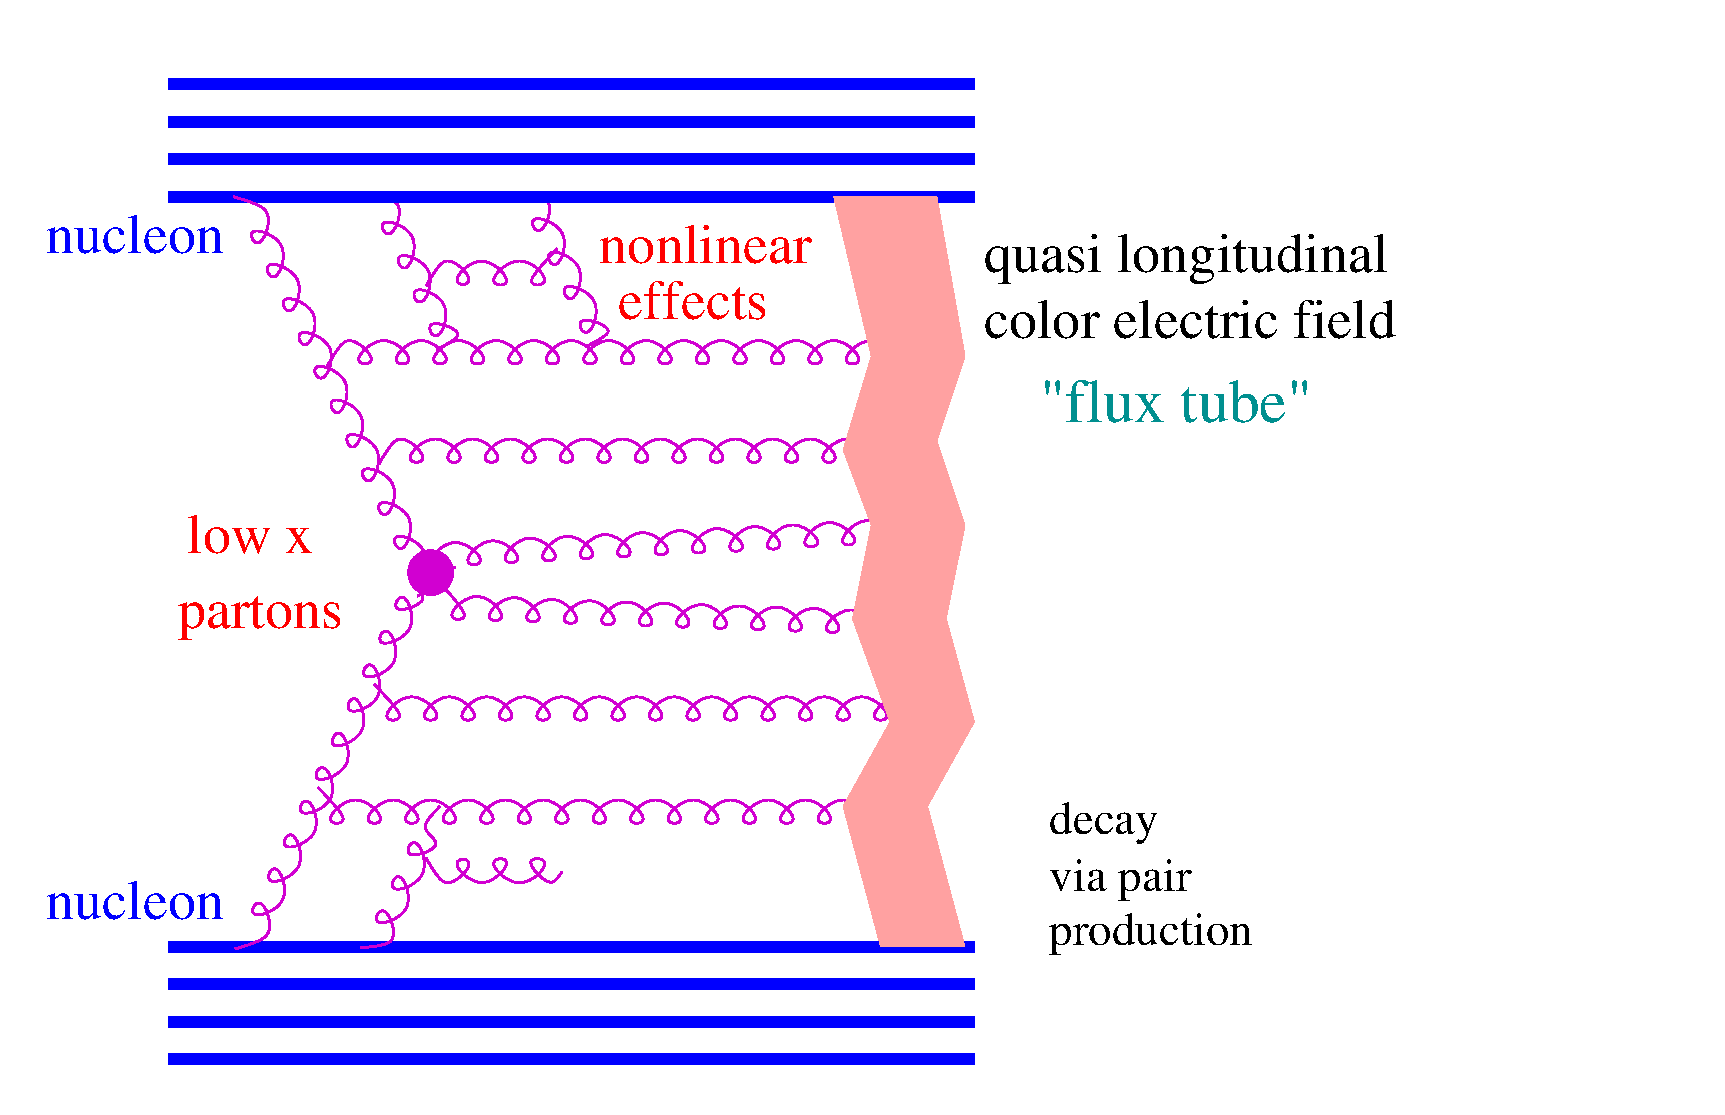
\includegraphics[width=.49\textwidth]{\imgpath/flux.eps}}}
\subfloat[][]{\adjustbox{valign=m}{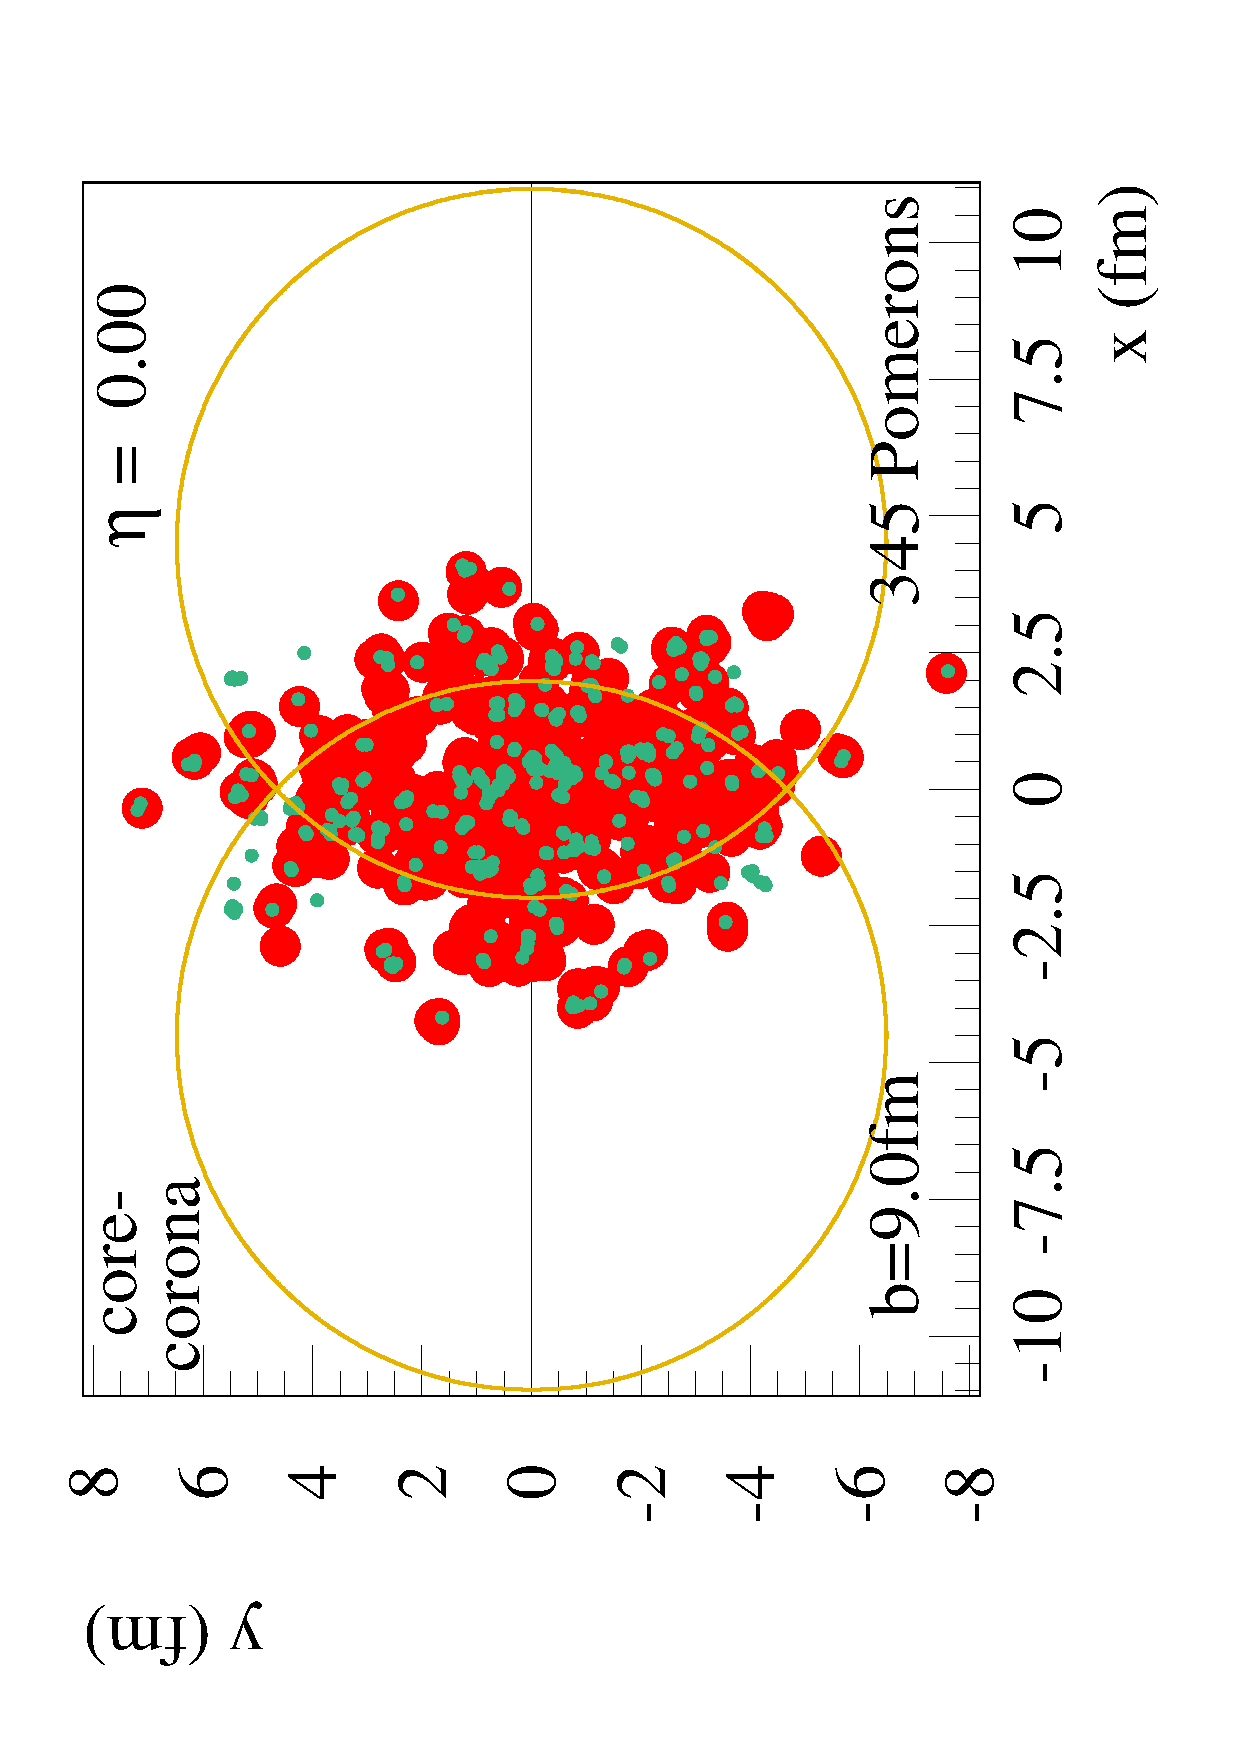
\includegraphics[width=.39\textwidth]{\imgpath/core1.pdf}}}\\
\subfloat[][]{\adjustbox{valign=m}{\includegraphics[width=.39\textwidth]{\imgpath/coco_ratio.pdf}}}
\caption{\textbf{(a)} Illustration of the partonic structure in the form of a parton ladder. \cite{pierogEPOSLHCTest2015} \textbf{(b)} Visualisation of the core (red) and corona (green) components in a peripheral $20-40\%$ collision of Pb-Pb with 345 initial multiple scatterings, modelled by EPOS3 \cite{knospeHadronicResonanceProduction2016} \textbf{(c)} Fractions of particle production associated with the core (red) and corona (blue) regions in p-Pb and Pb-Pb collisions, modelled by EPOS3. \cite{knospeHadronicResonanceProduction2021}}
\label{fig:colls:epos}
\end{figure}

\part{Experimental Setup and Methodology}
\chapter{Large Hadron Collider}
\def \imgpath {"./figures/lhc"}

\textit{This chapter is currently unfinished and needs a lot of work.}

\section{European Organisation for Nuclear Research}
CERN, located near Geneva, Switzerland, is an esteemed scientific institution dedicated to the study of particle physics, nuclear physics, and related fields. Established in 1954 by a consortium of European countries, it currently has 23 member states and collaborates with over 50 countries worldwide. Its research endeavors focus on advancing our understanding of the fundamental particles and forces that govern them.

One of the most significant and celebrated discoveries made by CERN is the Higgs boson, a particle that confers mass to other particles and is a crucial component of the Standard Model of particle physics. This discovery was made in 2012 by the ATLAS and CMS experiments, two of the four main experiments at CERN's Large Hadron Collider (LHC), the world's largest and most powerful particle accelerator.

Apart from the LHC, CERN houses several research facilities, including the Proton Synchrotron and the Super Proton Synchrotron, that provide beams of particles for a wide range of experiments. %In sum, CERN is a preeminent international center for pioneering research in particle physics and allied domains, and its findings and technological advancements have contributed substantially to our understanding of the universe. Furthermore, it embodies the potency of international collaboration and cooperation in scientific exploration.

\section{Large Hadron Collider (LHC)}

The Large Hadron Collider (LHC) is a particle accelerator that utilizes a circular tunnel with a circumference of 27 kilometers to accelerate beams of protons or heavy ions to high energies and collide them at four separate experimental locations. The LHC operates on the principle of accelerating these beams to nearly the speed of light through a series of superconducting magnets and then directing them to collide with each other at specific points along the circular path.

The LHC's superconducting magnets are cooled to temperatures close to absolute zero (-271.3 degrees Celsius) to maintain their superconducting state, allowing them to guide and focus the particle beams as they travel along the circular path. These magnets produce a strong magnetic field that keeps the particle beams on their circular trajectory and causes them to bend as they pass through the magnetic field. By adjusting the strength of the magnetic field, the LHC can control the curvature of the particle beams and ensure that they collide at the designated interaction points.

The LHC's acceleration process occurs in a series of stages, starting with a source of particles that are injected into a linear accelerator (LINAC). The LINAC accelerates the particles to an energy of a few million electronvolts (MeV) before passing them to a circular accelerator called a Booster. The Booster further accelerates the particles to an energy of 1.4 billion electronvolts (GeV) before injecting them into the Proton Synchrotron (PS).

The PS is a circular accelerator that increases the energy of the particles to 25 GeV before injecting them into the Super Proton Synchrotron (SPS). The SPS is a larger circular accelerator that further accelerates the particles to 450 GeV before finally injecting them into the LHC. Once inside the LHC, the particles are accelerated to their final energy and directed to collide at the designated interaction points.

The collisions at the LHC produce a shower of subatomic particles that are captured and analyzed by the LHC's four primary detectors: ATLAS, CMS, LHCb, and ALICE. These detectors are designed to measure the properties and trajectories of the particles produced by the collisions and provide valuable insights into the fundamental nature of matter and the universe.

Overall, the operational principle of the LHC is based on the precise control of the particle beams through a series of superconducting magnets and accelerators to produce high-energy collisions that enable cutting-edge research in particle physics.

The LHC tunnel is situated approximately 100 meters underground, in a tunnel that was previously used by the Large Electron-Positron Collider (LEP). It has a diameter of 3.8 meters and houses over 1,600 superconducting magnets. The collider operates for periods of several months at a time, with periods of downtime in between for maintenance and upgrades.

TBA Luminosity, bunches, Van der Meer scans

\begin{figure}%[!h]
\centering%
\includegraphics[width=.7\textwidth]{\imgpath/cern.png}
\caption{TBA.}
\label{fig:experiment:cern}
\end{figure}


\begin{figure}%[!h]
\centering%
\includegraphics[width=.7\textwidth]{\imgpath/dipole.jpg}
\caption{TBA.}
\label{fig:experiment:cern}
\end{figure}
\chapter{The ALICE Detector}
%\def \imgpath {"./figures/alice"}

The experimental measurements conducted as part of this dissertation in Chapters~\ref{chap:sphero} and \ref{chap:rt} have been carried out on data from proton-proton collisions at the Large Hadron Collider at CERN, collected with the ALICE detector. The aim of this chapter is to introduce these facilities.

\section{CERN and the LHC}

\textit{Conseil européen pour la recherche nucléaire} (CERN) is a scientific institution dedicated to study particle physics, nuclear physics, and related fields. It was established in 1954 as a European collaborative endeavour and currently has 23 member states. The CERN laboratories employ almost 3000 on-site staff and host approx.\ 13000 users from universities and research institutions across the world. The biggest achievments of CERN include discoveries of the $W^\pm$, $Z^0$, \cite{cashmorePrestigiousDiscoveriesCERN2003} and the Higgs bosons \cite{thecmscollaborationObservationNewBoson2012, theatlascollaborationObservationNewParticle2012}, the first creation of anti-atoms, advancements to proton therapy and medical imaging technologies such as PET, and finally, being a birthplace to the World Wide Web.

The Large Hadron Collider (LHC) is the main particle accelerator at CERN. This synchrotron with circumference of almost 27 km can accelerate protons to energies up to $7$~TeV, making it world's most powerful particle accelerators. Apart from collisions of protons measured at \sppt{13}, it also studies collisions of nuclei, such as lead (Pb-Pb) at \snnt{5.02}, or proton-lead p-Pb at \snnt{8.16}. Particles in the synchrotron are accelerated by electric fields within RF cavities and kept on their semi-circular trajectory using magnetic dipoles. Higher-polar magnets are used for beam focusing and adjustment. The particles circulate in larger bunches (of $\sim 10^{11}$ protons or $\sim 7\times10^7$ Pb nuclei) in two separate rings, which intersect at sites of large experiments, detecting their collisions. Apart from ALICE, discussed in the next sections, these are:
\begin{itemize}
\item \textbf{ATLAS} (\textit{A Toroidal LHC ApparatuS}) \cite{collaborationATLASExperimentCERN2008}: the LHC's largest experiment and a general purpose detector, with its foci including Higgs physics, scrutiny of the SM, and BSM searches.
\item \textbf{CMS} (\textit{Compact Muon Solenoid}) \cite{collaborationCMSExperimentCERN2008}: also a general purpose detector, with similar physics goals, but with a different technical design than ATLAS. It has also been a prominent contributor to QGP physics, particularly the study of small systems.
\item \textbf{LHCb} (\textit{Large Hadron Collider beauty}) \cite{collaborationLHCbDetectorLHC2008}: a detector focused mostly on precise measurements of b physics and CP violation. 
\end{itemize}

\begin{table}[h!]
\centering
\caption{Selection of parameters of the Large Hadron Colliders. \cite{schmidtProtectionCERNLarge2006} }
\label{tab:alice:lhcpars}
\begin{tabular}{|cc|c|}
\hline
\multicolumn{2}{|c|}{\parbox[b][1.2em]{2em}{} Parameter} & Value \\ \hline
\multicolumn{2}{|l|}{\parbox[b][1.1em]{1em}{}Circumference} &  $26.7$ km\\ \hline
\multicolumn{2}{|l|}{\parbox[b][1.1em]{1em}{}Energy at injection} &  $450$ GeV\\ \hline
\multicolumn{2}{|l|}{\parbox[b][1.1em]{1em}{}Magnetic field at 7 TeV} &  $\sim 8.3$ T\\ \hline
\multicolumn{2}{|l|}{\parbox[b][1.1em]{1em}{}Number of magnets} &  $\sim 9300$\\ \hline
\multicolumn{2}{|l|}{\parbox[b][1.1em]{1em}{}Revolution frequency} &  $\sim 11$ kHz\\ \hline
\multicolumn{2}{|l|}{\parbox[b][1.1em]{1em}{}Number of bunches in a beam} &  $2808$\\ \hline
\multicolumn{2}{|l|}{\parbox[b][1.1em]{1em}{}Bunch spacing} &  $25$ ns\\ \hline
\multicolumn{2}{|l|}{\parbox[b][1.1em]{1em}{}Design luminosity} &  $\sim 10^{34} \, \mathrm{cm^{-2}s^{-1}}$\\ \hline
\multicolumn{2}{|l|}{\parbox[b][1.1em]{1em}{}Max.\ bunch crossing (BC) rate} &  $\sim 40$ MHz\\ \hline
\multicolumn{2}{|l|}{\parbox[b][1.1em]{1em}{}Number of inel.\ interactions per BC} &  $10-20$\\ \hline
\multicolumn{2}{|l|}{\parbox[b][1.1em]{1em}{}Beam lifetime} &  $\sim 10$ h\\ \hline
\end{tabular}
\end{table}

Some of the LHC parameters are summarised in Tab.~\ref{tab:alice:lhcpars} and an aerial photo of the LHC with locations of the IPs can be seen in Fig.~\ref{fig:alice:lhc}.

\begin{figure}%[!h]
\subfloat[][]{\adjincludegraphics[trim={0 {.18\height} 0 {.07\height}},clip,width=.8\textwidth]{\imgpath/lhc.jpg}}\\
\subfloat[][]{\adjincludegraphics[trim={0 {.08\height} 0 {.07\height}},clip,width=.8\textwidth]{\imgpath/ip.jpg}}
\caption{\textbf{(a)} Aerial photo of the LHC area, also depicting the location of the LHC tunnel (approx.\ $100$~m underground), spanning over Switzerland and France. Geneva, Lac Léman, and the Mont Blanc can be seen in the background. \cite{briceAerialViewCERN2008} \textbf{(b)} Visualisation of the beam crossing at the ALICE experiment. Bunches of Beam 1 move from left to right in the blue beam envelope and bunches of Beam 2 move from right to left in the red beam envelope. The envelopes indicate the beam orbits and transverse size. \cite{LHCReportMake2023}}
\label{fig:alice:lhc}
\end{figure}

\section{The ALICE experiment}

The ALICE (A Large Ion Collider Experiment) \cite{collaborationALICEExperimentCERN2008, PerformanceALICEExperiment2014} is the detector at the LHC dedicated to studying collisions of heavy nuclei and the properties of QCD matter, such as quark-gluon plasma. Its biggest strengths are precise tracking and momentum determination all the way down to $\pt>\gevc{0.15}$ as well as superior particle identification (PID). Its sub-detectors are subjected to a magnetic field of $0.5$~T to allow momentum measurements from the track curvatures (in natural units, $\pt \approx 0.3 B r, \, \pt \in [\gevc{}], \, B \in [\mathrm{T}], \, r \in [\mathrm{m}]$).

The ALICE detector, shown in Fig.~\ref{fig:alice:alice}, consists of several sub-systems, each fulfilling their function. Some of them which pertain to the measurements carried out within this dissertation are listed in Tab.~\ref{tab:alice:alice}. The following descriptions are based on their status when the data was collected, which corresponds to Run~2.

\begin{figure}[H]
\centering%
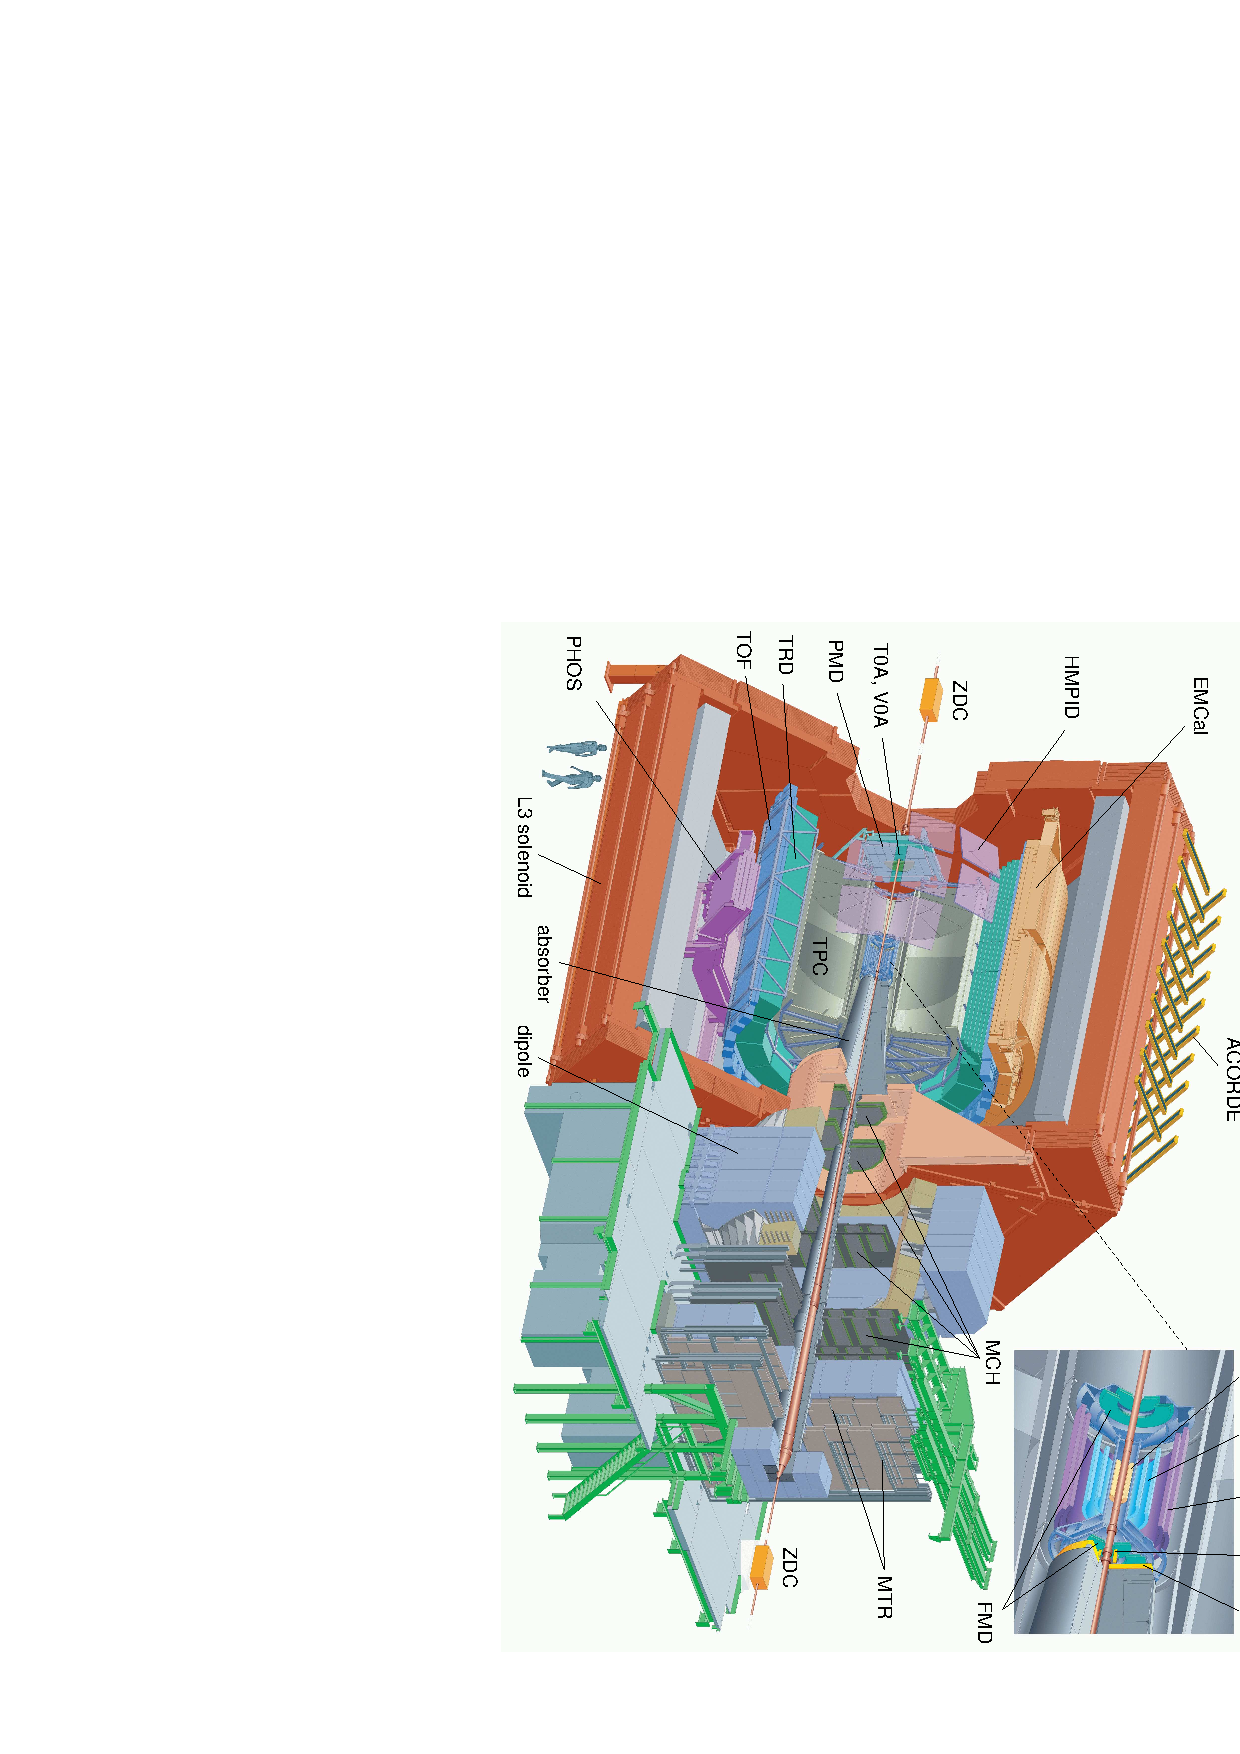
\includegraphics[width=.99\textwidth]{\imgpath/setup7.pdf}
\caption{The ALICE experiment at the LHC, showing its sub-systems. The central barrel is subjected to a magnetic field from the solenoid (red). The ZDC detectors are approximately $\pm 113$~m distant from the IP. \cite{alicecollaborationPerformanceALICEExperiment2014}}
\label{fig:alice:alice}
\end{figure}

\begin{table}[h!]
\centering
\caption{Selection of ALICE sub-detectors relevant to this thesis. Acceptance is given in terms of pseudorapidity, the azimuthal coverage for the detectors presented is full. The $z$-axis is defined anticlockwise to the LHC. \cite{alicecollaborationPerformanceALICEExperiment2014} }
\label{tab:alice:alice}
\begin{tabular}{|cc|cccc|}
\hline
\multicolumn{2}{|c|}{\parbox[b][1.2em]{2em}{} Detector} & Acceptance & Position (cm) & Technology & Main purpose \\ \hline
\multicolumn{6}{l}{\parbox[b][0.2em]{1em}{}} \\
\hline
\multicolumn{2}{|c|}{\parbox[b][1.2em]{2em}{} ITS SPD} & $|\eta|<2.0$ & $r=3.9$ cm & Si pixel & tracking, PV, triggering \\
\multicolumn{2}{|c|}{\parbox[b][1.2em]{2em}{} ITS SPD} & $|\eta|<1.4$ & $r=7.6$ cm & Si pixel & tracking, PV, triggering \\
\hline
\multicolumn{2}{|c|}{\parbox[b][1.2em]{2em}{} ITS SDD} & $|\eta|<0.9$ & $r=15.0$ cm & Si drift & tracking, PID \\
\multicolumn{2}{|c|}{\parbox[b][1.2em]{2em}{} ITS SDD} & $|\eta|<0.9$ & $r=23.9$ cm & Si drift & tracking, PID \\
\hline
\multicolumn{2}{|c|}{\parbox[b][1.2em]{2em}{} ITS SSD} & $|\eta|<1.0$ & $r=38.0$ cm & Si strip & tracking, PID \\
\multicolumn{2}{|c|}{\parbox[b][1.2em]{2em}{} ITS SSD} & $|\eta|<1.0$ & $r=43.0$ cm & Si strip & tracking, PID \\
\hline
\multicolumn{2}{|c|}{\parbox[b][1.2em]{2em}{} TPC} & $|\eta|<0.9$ & $r=85.0$ cm & Ne drift, MWPC & tracking, PV, PID \\
\hline
\multicolumn{2}{|c|}{\parbox[b][1.2em]{2em}{} \VOA} & $2.8<|\eta|<5.1$ & $z=329.0$ cm & scintillator & centrality, triggering \\
\multicolumn{2}{|c|}{\parbox[b][1.2em]{2em}{} \VOC} & $-3.7<|\eta|<-1.7$ & $z=-88.0$ cm & scintillator & centrality, triggering \\
\hline
\end{tabular}
\end{table}


\section{Time Projection Chamber}

The Time Projection Chamber (TPC) \cite{peskovTechnicalDesignReport2014} is ALICE's primary tracking detector and investigation tool for hadronic observables. It is located in the central barrel. The cylinder, illustrated in Fig.~\ref{fig:alice:tpc} is filled with a mixture of gases and a central $100$-kV high-voltage electrode subjects it to a longitudinal electric field. Charged particles traversing the gas medium ionise it and the electrons then drift to the end-caps with a drift time of approx.\ $90 \, \mathrm{\mu s}$. There, they are detected in Read-out Chambers (ROCs), using Multi-Wire Proportional Chambers (MWPC), and together with the drift duration time, a three-dimensional information can be determined. The ROCs are radially divided (IROCs and OROCs) and segmented into 18 sectors in azimuth. Each ROC has 159 rows and its signals are processed by attached Front-End Cards (FECs). The MWPC principle and the ROC design, visualised with a charged particle track crossing all its rows, can be seen in Fig.~\ref{fig:alice:rocs}.

In addition to the tracking information, the TPC is also used in PID, by measuring the charged particles' specific ionisation loss $\mathrm{d}E/\mathrm{d}x$. Measurements of $\mathrm{d}E/\mathrm{d}x$ for different particle species as a function of the particle momentum and charge is displayed in Fig.~\ref{fig:alice:tpc}. A selection of TPC parameters not discussed above is given in Tab.~\ref{tab:alice:tpc}.

\begin{table}[h!]
\centering
\caption{Selection of parameters of the Time Projection Chamber. \cite{collaborationALICEExperimentCERN2008} }
\label{tab:alice:alice}
\begin{tabular}{|cc|c|}
\hline
\multicolumn{2}{|c|}{\parbox[b][1.2em]{2em}{} Parameter} & Value \\ \hline
\multicolumn{2}{|l|}{\parbox[b][1.1em]{1em}{}Radial position (active volume)} &  $84.8<r<246.6$ cm\\ \hline
\multicolumn{2}{|l|}{\parbox[b][1.1em]{1em}{}Length (active volume)} &  $2\times250$ cm\\ \hline
\multicolumn{2}{|l|}{\parbox[b][1.1em]{1em}{}Detector gas} &  Ne/CO$_2$/N$_2$ or Ar/CO$_2$\\ \hline
\multicolumn{2}{|l|}{\parbox[b][1.1em]{1em}{}Spatial resolution} &  $0.8-1.1$ mm in $r\phi$\\
\multicolumn{2}{|l|}{\parbox[b][1.1em]{1em}{} } &  $1.1-1.2$ mm in $z$\\ \hline
\multicolumn{2}{|l|}{\parbox[b][1.1em]{1em}{}$\mathrm{d}E/\mathrm{d}x$ resolution} &  $\sim 5.0\%$\\ \hline
\multicolumn{2}{|l|}{\parbox[b][1.1em]{1em}{}Material budget $X/X_0$} &  $3.5\%$ near $\eta=0$\\ \hline
\end{tabular}
\end{table}

\begin{figure}[!h]
\subfloat[][]{\adjustbox{valign=m}{\includegraphics[width=.47\textwidth]{\imgpath/tpc.png}}}
\subfloat[][]{\adjustbox{valign=m}{\includegraphics[width=.47\textwidth]{\imgpath/dedx.eps}}}
\caption{\textbf{(a)} Illustration of the TPC detector. \cite{peskovTechnicalDesignReport2014}. \textbf{(b)} Ionisation energy loss of charged particles as a function of their momentum normalised by their charge as determined by the TPC. The dashed lines represent predictions from calculations. \cite{alicecollaborationPerformanceALICEExperiment2014}}
\label{fig:alice:tpc}
\end{figure}

\begin{figure}[!h]
\subfloat[][]{\adjustbox{valign=m}{\includegraphics[width=.45\textwidth]{\imgpath/mwpc.png}}}
\subfloat[][]{\adjustbox{valign=m}{\includegraphics[width=.45\textwidth]{\imgpath/fec2.png}}}
\caption{\textbf{(a)} Depiction of the operating principle at the ROCs, using MWPC. \cite{kalweitProductionLightFlavor2012} \textbf{(b)} The IROC (bottom part) and OROC (top part) visualised with their number of rows and the signal-processing FECs. Also shown is a charged particle trajectory (red), which in this case crosses all 159~rows. \cite{peskovTechnicalDesignReport2014} (\textit{modified})}
\label{fig:alice:rocs}
\end{figure}


\subsection{Upgrade for Run 3: GEM read-outs}

In the Run 2 setup, to avoid build-up of space charge in the TPC due to backflow of ions from the amplification region in MWPCs, a gating grid is used. This limits the operating rate of the TPC to approx.\ $3.5$~kHz. However, for the Run 3 operation, the TPC has been planned to enable a continous read-out mode of Pb-Pb collisions at the interaction rate $50$~kHz. For this reason, a new read-out technology, the Gas Electron Multiplier (GEM), is used. The technology and upgraded are discussed in more detail in Ref.~\cite{adolfssonUpgradeALICETPC2021}. Commissioning of this upgraded TPC comprised the author's qualification task.

The GEM uses $50$-$\mathrm{\mu m}$ thin foils of insulating material, coated with conductive layers of thickness $2-5$ $\mathrm{\mu m}$ at each side, to which a potential difference of $200-400$~V is applied. The foil is perforated with double-conical holes of diameters $\sim 70$ and $\sim 50$ $\mathrm{\mu m}$ and a pitch of $\sim 140$ or $\sim 280$~$\mathrm{\mu m}$. The electric field in the holes than causes avalanche multiplication. Four GEM layers are stacked on top of each other in a way, where the holes have different positions and densities, which reduces the ion backflow. Typically, for one electron, the gain is around $2000$, with $20$ ions flowing back into the drifting region. The GEM setup at ALICE is displayed in Fig.~\ref{fig:alice:gems}.

\begin{figure}[!h]
\subfloat[][]{\adjustbox{valign=m}{\includegraphics[width=.38\textwidth]{\imgpath/gem1.png}}}\hspace{1em}
\subfloat[][]{\adjustbox{valign=m}{\includegraphics[width=.38\textwidth]{\imgpath/gem2c.png}}}\\
\subfloat[][]{\adjustbox{valign=m}{\includegraphics[width=.583\textwidth]{\imgpath/gem3.png}}}
\caption{\textbf{(a)} Electron microscope photograph of a GEM foil with hole pitch 140~$\mu$m. \cite{kalweitProductionLightFlavor2012} \textbf{(b)} Simulation of the charges in GEM holes. Dark lines represent ions and light lines electrons. Green dots mark multiplication site. \textbf{(c)} Schematic of the GEM setup at the upgraded ALICE TPC. \cite{peskovTechnicalDesignReport2014}}
\label{fig:alice:gems}
\end{figure}

\section{Inner Tracking Systems}

The Inner Tracking System \cite{collaborationALICEExperimentCERN2008, alicecollaborationAlignmentALICEInner2010} is a set of semiconductor-based detectors also located in the central barrel, but much closer to the beam pipe. ALICE uses the ITS for its great spatial resolution, which complements the TPC tracking and allows for precise determination of the primary vertex (PV) as well as secondary vertices of short-lived particle decays. Moreover, thanks to its fast processing, it is also used for triggering. The ITS consists of three detectors, each of two layers, which use different silicon detector technologies:
\begin{itemize}
\item Silicon Pixel Detector (SPD): uses an extremely granular pixel matrix closest to the IP, where particle densities are the highest.
\item Silicon Drift Detector (SDD): uses a similar technology based on drift cells. It is slightly less granular than the SPD but allows measuring of the deposited charge and thus PID based on $\mathrm{d}E/\mathrm{d}x$.
\item Silicon Strip Detector (SSD): uses a silicon detector with two arrays of strips, misaligned with $\Delta\phi \approx 2 \deg$, forming a lattice, on which a spatial coordinate can be determined. Similarly to the SDD, $\mathrm{d}E/\mathrm{d}x$ can also be measured.
\end{itemize}
Important parameters of the ITS sub-system can be found in Tab.~\ref{tab:alice:its} and the operating principles of the different silicon-based detector technologies used is discussed e.g.\ in Ref.~\cite{krammerSiliconDetectorsHigh2015, masciocchiLectureNotesSemiconductor2017}.

\begin{table}[h!]
\centering
\caption{Selection of parameters of the Inner Tracking System. \cite{collaborationALICEExperimentCERN2008}}
\label{tab:alice:its}
\begin{tabular}{|cc|ccc|}
\hline
\multicolumn{2}{|r|}{\parbox[b][1.2em]{2em}{} Detector} & SPD & SDD & SSD \\ \hline
\multicolumn{5}{l}{\parbox[b][1.2em]{1em}{} Parameter} \\
\hline
\multicolumn{2}{|l|}{\parbox[b][1.1em]{1em}{}Area (m$^2$)} & $0.07$ and $0.14$ & $0.42$ and $0.89$ & $2.09$ and $2.68$\\ \hline
\multicolumn{2}{|l|}{\parbox[b][1.1em]{1em}{}Cell size ($\mu$m)} & $50\times 425$ & $150\times 300$ & $95\times 40000$\\ \hline
\multicolumn{2}{|l|}{\parbox[b][1.1em]{1em}{}Number of cells (M)} & $9.84$ & $23$ & $2.6$\\ \hline
\multicolumn{2}{|l|}{\parbox[b][1.1em]{1em}{}Spatial resolution ($\mu$m)} & $12$ in $r\phi$, $100$ in $z$ & $38$ in $r\phi$, $28$ in $z$ & $20$ in $r\phi$, $830$ in $z$\\ \hline
\multicolumn{2}{|l|}{\parbox[b][1.1em]{1em}{}Mat.\ budget, layers $X/X_0$} & $1.14\%$ and $1.14\%$ & $1.13\%$ and $1.26\%$ & $0.83\%$ and $0.86\%$\\ \hline
\multicolumn{2}{|l|}{\parbox[b][1.1em]{1em}{}Mat.\ budget, supp.\ $X/X_0$} & $0.52\%$ & $0.25\%$ & $0.53\%$\\ \hline
\end{tabular}
\end{table}

\begin{figure}[!h]
\subfloat[][]{\adjustbox{valign=m}{\includegraphics[width=.45\textwidth]{\imgpath/its.pdf}}}%\hspace{1em}
\subfloat[][]{\adjustbox{valign=m}{\includegraphics[width=.45\textwidth]{\imgpath/itscosmic.pdf}}}
\caption{\textbf{(a)} Three-dimensional model of the ITS sub-system in ALICE detector simulations. \textbf{(b)} Display of a cosmic event detected by the ITS. \cite{alicecollaborationAlignmentALICEInner2010}}
\label{fig:alice:its}
\end{figure}

\section{\VOA and \VOC}

The \VOA and \VOC\footnote{In ALICE, the ``A-side" points in the counter-clockwise and the ``C-side" in the clockwise direction of the LHC beam pipe, aligned with the $z$-axis. The C-side contains the muon system.} are two arrays of plastic scintillator counters, with PMT read-outs, together forming the V$0$ sub-system \cite{alicecollaborationPerformanceALICEVZERO2013}. They are placed asymmetrically on the $z$-axis with respect to the IP in order to accomodate the hadron absorber used in the muon tracking system of ALICE. Their inner and outer radii are $4.3$ and $42.2$~cm for the \VOA and $4.5$ and $32$~cm for the \VOC. Furthermore, they are segmented into 8 sectors azimuthally and 4 sectors radially. This is usually not granular enough for tracking, but sufficient for forward multiplicity estimation (combining amplitudes of both parts, referred to as \VOM) or determination of the event plane. 

Thanks to its speed, the V$0$ is also used for triggering. Additionally, since they can be used in coincidence, interactions of the protons/nuclei with residual gas in the beam pipe outside of the IP can be identified based on the different time information and rejected. The two detectors are visualised in Fig.~\ref{fig:alice:vzero}.

\begin{figure}[!h]
\includegraphics[width=.65\textwidth]{\imgpath/vzero.eps}\caption{Schematic of the \VOA and \VOC scintillator arrays. \cite{alicecollaborationPerformanceALICEVZERO2013}}
\label{fig:alice:vzero}
\end{figure}

\chapter{Events, Vertices, Tracks, and Particles}
\input{chapters/blank}

\part{Author's measurements}
\chapter{Reconstruction of neutral strange particles with ALICE}
\%input{chapters/analysis}
\chapter{Transverse Spherocity}
%\def \imgpath {"./figures/sphero"}
In this chapter, measurements of \KOs, \LA, and \AL are reported as a function of transverse spherocity \SOPT. It is defined as
\begin{align}
\SOPT = \frac{\pi^2}{4} \min_{\hat{n}} \left(\frac{\sum_i
      |\hat{p_{\textrm{T},i}} \times \hat{n}|}{N_{\textrm{trks}}}  \right) \quad ,
\end{align}
where $\hat{p_{\textrm{T},i}}$ represents the unit vector of transverse momentum of a particle $i$, $N_{\textrm{trks}}$ the number of charged particles entering the sum, and $\hat{n}$ is the event-dependent unit vector which minimises the sum. The sum runs over all charged particles in the event within $|\eta|<0.8$ and with $\pt > 0.15$~\gevc \ .
\section{Understanding transverse spherocity}

TBA: Illustrating isotropic and jetty event.

TBA: Motivation for studying \SOPT

TBA: Motivation for unweighted spherocity

\begin{figure}%
\subfloat[][]{\includegraphics[width=.60\textwidth]{\imgpath/SO_Unfolded_CL1_Perc_1.pdf}}\\
\subfloat[][]{\includegraphics[width=.60\textwidth]{\imgpath/SO_Unfolded_CL1_Perc_10.pdf}}\\
\subfloat[][]{\includegraphics[width=.60\textwidth]{\imgpath/SO_Unfolded_V0M_Perc_1.pdf}}\\
\caption{The measured and fully corrected \SOPT distributions for both \textbf{(a)} \NSPD 0--1\%, \textbf{(b)} 0--10\% and \textbf{(c)} \VOM 0--1\% . The curves represent different model prediction, where the shaded area represents the statistical uncertainty of the models.}
\label{fig:sphero:sopt}
\end{figure}

\section{Transverse momentum spectra}

The corrected spectra in \VOM, and CL1 events and the dependence on spherocity for the \KOs and \LA + \AL can be seen in Fig.~\ref{fig:sphero:k0spt} and Fig.~\ref{fig:sphero:lpt}, respectively.

\begin{figure}%[!h]
\centering%
\includegraphics[height=.3\textheight]{\imgpath/sp_K0s_V0M01_spher10.pdf}
\includegraphics[height=.3\textheight]{\imgpath/sp_K0s_NCharged01_spher10.pdf}
\includegraphics[height=.3\textheight]{\imgpath/sp_K0s_NCharged_spher1.pdf}
\includegraphics[height=.3\textheight]{\imgpath/sp_K0s_V0M01_spher1.pdf}
\includegraphics[height=.3\textheight]{\imgpath/sp_K0s_NCharged01_spher1.pdf}
  \caption{Corrected and normalised \pt -spectra of the \KOs particle in high-multiplicity \VOM 0-1\%(\textit{top left, bottom left}), CL1 0-1\% (\textit{top middle, bottom right}), and CL1 0-10\% (\textit{top right}) events, shown as black points. The bottom (jetty) and top (isotropic) 1\% or 10\% of spherocity events are also shown as red and blue points. The ratios of isotropic/jetty spectra to the high-multiplicity spectra are shown in the bottom panels.}
\label{fig:sphero:k0spt}
\end{figure}

\begin{figure}%[!h]
\centering%
\includegraphics[height=.3\textheight]{\imgpath/sp_LLbar_V0M01_spher10.pdf}
\includegraphics[height=.3\textheight]{\imgpath/sp_LLbar_NCharged01_spher10.pdf}
\includegraphics[height=.3\textheight]{\imgpath/sp_LLbar_NCharged_spher1.pdf}
\includegraphics[height=.3\textheight]{\imgpath/sp_LLbar_V0M01_spher1.pdf}
\includegraphics[height=.3\textheight]{\imgpath/sp_LLbar_NCharged01_spher1.pdf}
  \caption{Corrected and normalised \pt -spectra of the \LA + \AL particles in high-multiplicity V0M 0-1\%(\textit{top left, bottom left}), CL1 0-1\% (\textit{top middle, bottom right}), and CL1 0-10\% (\textit{top right}) events, shown as black points. The bottom (jetty) and top (isotropic) 1\% or 10\% of spherocity events are also shown as red and blue points. The ratios of isotropic/jetty spectra to the high-multiplicity spectra are shown in the bottom panels.}
\label{fig:sphero:lpt}
\end{figure}

\chapter{Underlying Event Activity}
%\label{chap:rt}
\def \imgpath {"./figures/rt"}

In this chapter, measurements of \KOs, \LA, and \AL are reported as a function of the underlying event activity classifiers \RT, \RTmin, and \RTmax. These observables quantify the magnitude of the underlying event and are an experimental proxy of the number of Multiple Partonic Interactions, \nmpi.

\section{Motivation for studying event sub-structure}

\subsection{Underlying event}

As discussed in Section~\ref{sec:intro:ue}, the underlying event is composed of particles that are not directly related to the primary hard scattering and its related fragmentation. It can be studied to extract accurate information about the hard scattering process by subtracting it in precision measurements of jet properties. Moreover, since it is a manifestation of the proton substructure and the parton interactions, it can give us insight into the parton dynamics in the nonperturbative QCD region.

%In theory chapter, discuss UE history:
%J. R. Cudell et al., "Experimental study of the underlying event in high transverse momentum jet production at the CERN ISR", Nuclear Physics B, Volume 336, Issue 1, Pages 1-21 (1990). DOI: 10.1016/0550-3213(90)90568-V
%CDF Collaboration, "Observation of the Underlying Event in Dijet Events with a Leading Transverse Energy Jet at the Collider Detector at Fermilab", Physical Review Letters, Volume 83, Issue 7, Pages 1183-1188 (1999). DOI: 10.1103/PhysRevLett.83.1183
%DELPHI Collaboration, "Measurement of the underlying event in hadronic Z0 decays", Physics Letters B, Volume 382, Issues 3–4, Pages 323-332 (1996). DOI: 10.1016/0370-2693(96)00620-1

\subsection{Hard process--multiplicity bias}

Studying QGP phenomena in small systems as a function of event activity is challenging due to selection biases that arise when analyzing the data. It is known that selecting events with large momentum transfer leads to a bias towards higher multiplicities (and underlying event) \cite{alicecollaborationConstraintsJetQuenching2018}, and conversely, selecting events with higher multiplicities (and UE) enhances the hard processes \cite{alicecollaborationMultiplicityDependenceChargedparticle2022}. This bias can be understood in several ways. Firstly, a hard process tends to occur with lower impact parameters, which in turn leads to higher particle multiplicities. Secondly, an event with $n$ partonic interactions has $n$ chances of containing a hard process. Lastly, harder processes fragment into more particles, further contributing to higher event activity. As an example, Figure~\ref{fig:rt:hardbias} shows how the requirement of a high \pt track can skew the forward-rapidity centrality distribution to lower values (higher event activity), as observed in a result from ALICE \cite{alicecollaborationConstraintsJetQuenching2018}.

\begin{figure}%
\subfloat[][]{\includegraphics[width=.480\textwidth]{\imgpath/alice_hard_multi_bias.pdf}}\\
\caption{Distribution of event activity measured at forward rapidity (\VOA percentile) for minimum bias events (blue points) and for events requiring a high-\pt trigger in the intervals $6<\pt<\gevc{7}$ (black points) and $12<\pt<\gevc{50}$ (red points). Lower \VOA percentile represent higher event activity. The MB distribution is trivally uniform by construction. \cite{alicecollaborationConstraintsJetQuenching2018}}
\label{fig:rt:hardbias}
\end{figure}

\subsection{Azimuthal regions and transverse activity}

The selection bias of hard processes on UE becomes saturated at high \pt, where the impact parameter bias is fixed and stochastic effects become comparable \cite{acharyaUnderlyingEventProperties2020}. This saturation effect can be observed when studying particle production in three topological regions defined with respect to the highest momentum track, which serves as a proxy for the axis of the primary scattering process. The three regions are defined as follows:
\begin{enumerate}
\item Towards (also known as "Near"), where $|\phi - \philead| < \frac{\pi}{3}$,
\item Away, where $|\phi - \philead| > \frac{2\pi}{3}$, and 
\item Transverse, where $\frac{\pi}{3} < |\phi - \philead| < \frac{2\pi}{3}$. 
\end{enumerate}
Here, \philead is the azimuthal angle of the leading track. This definition is illustrated in Figure~\ref{fig:rt:rtdefi}. 

\begin{figure}%
\subfloat[][]{\includegraphics[width=.490\textwidth]{\imgpath/rt_defi.png}}
\subfloat[][]{\includegraphics[width=.490\textwidth]{\imgpath/alice_uevpt.pdf}}\\
\caption{\textbf{(a)} Illustration of the three azimuthal regions: Toward, Away, Transverse; defined with respect to the highest-\pt track. \cite{acharyaUnderlyingEventProperties2020} \textbf{(b)} Charged particle density distributions as a function of \pt of the leading track in the three azimuthal regions. Error bars indicate statistical uncertainties and shaded areas represent systematic uncertainties. \cite{acharyaUnderlyingEventProperties2020} }
\label{fig:rt:rtdefi}
\end{figure}

Studying particle multiplicity (or sum of their \pt) in these regions as a function of the transverse momentum of the leading track \ptlead reveals that in the regions Towards and Away, the multiplicity continues to increase with the hardness of the primary process \cite{acharyaUnderlyingEventProperties2020, atlascollaborationMeasurementChargedparticleDistributions2017}. These regions contain the leading and the recoil jet, respectively. In contrast, in the Transverse region, the multiplicity (further denoted as $N_T$ in this thesis but $N_\mathrm{ch}^\mathrm{trans}$ is also used in cited literature) reaches a plateau at around $\gevc{5}$. In this region, the underlying event becomes independent of the strength of the primary process, and the selection bias is minimized. Notably, this phenomenon is universal regardless of the system size or collision energy \cite{atlascollaborationMeasurementChargedparticleDistributions2017, acharyaUnderlyingEventProperties2020, alicecollaborationUnderlyingEventMeasurements2012, alicecollaborationUnderlyingeventPropertiesPp2022}. As an example, measurements from ALICE are shown in Fig.~\ref{fig:rt:rtdefi}.

\section{\RT as an experimental observable}

The magnitude of the underlying event can be measured using the self-normalized ratio:
\begin{align}
\RT = \frac{\NT}{\langle \NT \rangle},
\end{align}
which is often referred to as the underlying event activity, transverse activity, or relative transverse activity in various literature \cite{martinProbingCollectiveEffects2016, alicecollaborationUnderlyingEventProperties2020, alicecollaborationProductionPionsKaons2023}, and also in this thesis. This observable and its uses were suggested in Ref.~\cite{martinProbingCollectiveEffects2016}.

By applying $\RT$, two limits of events can be studied:
\begin{itemize}
\item $\RT \rightarrow 0$: the \textbf{``ee"} limit, where events with minimal UE are selected. These events are dominated by a single hard scattering and can be compared to LEP fragmentation models.
\item $\RT \rightarrow \infty$: the \textbf{``AA"} limit, where events with very high transverse activity are selected, which can come from many MPIs and/or from transverse jets. These events may exhibit features similar to pA and AA collisions.
\end{itemize}

\subsection{Proxy to \nmpi}

As could be intuitively expected, \RT serves as an experimental proxy for \meannmpi. Phenomenological models that incorporate MPIs provide an illustration of this relationship. As shown in Fig.~\ref{fig:rt:nmpi}, Pythia 8 predicts a strong dependence of \meannmpi on \RT until $\RT \lesssim 5$. Similarly, Herwig 7 predicts a dependence until $\RT \lesssim 3$, albeit weaker. Pythia's prediction for the relationship between \RT and the event multiplicity, which is affine, is also shown in Fig.~\ref{fig:rt:nmpi}.

\begin{figure}%
\subfloat[][]{\includegraphics[width=.480\textwidth]{\imgpath/rt_minmax_nmpi.png}}
\subfloat[][]{\includegraphics[width=.465\textwidth]{\imgpath/rt_nch.png}}\\
\caption{\textbf{(a)} Dependence of the mean number of MPIs on the underlying event activity classifiers \RT, \RTmin, and \RTmax in pp collisions at \sppt{5.02}, as predicted by Pythia 8 (black) and Herwig 7 (red). \cite{bencediDisentanglingHardGluon2021} \textbf{(b)} Pythia 8 prediction for the correlation of the self-normalised charged particle multiplicity measured at mid-rapidity in events with a high-\pt trigger and the underlying event activity classifiers \RT, \RTmin, \RTmax. \cite{bencediDisentanglingHardGluon2021}}
\label{fig:rt:nmpi}
\end{figure}


\subsection{Extension to \RTmin, \RTmax}

Upon closer inspection of Fig.~\ref{fig:rt:rtdefi}, it can be observed that the charged particle multiplicity does not completely plateau in the Transverse region either, which was an important factor in motivating \RT measurements. Instead, there is a slight increase with \ptlead, although the effect is small. This rise can be attributed to harder, wide-angle ISR and FSR \cite{fieldUnderlyingEventHadronic2012}.

To separate the soft and hard components of the underlying event -- namely, the MPIs from wide-angle ISR/FSR -- the definition of \RT can be extended. The two transverse sub-regions can be further classified as Transverse-min or Transverse-max, based on which sub-region has fewer or more particles. Softer contributions from MPIs will enter both sub-regions, whereas harder radiation should affect mainly the Transverse-max sub-region. This makes Transverse-min more sensitive to particle production from MPIs. Figure~\ref{fig:rt:ue} illustrates how the Transverse-max region captures most of the rise of \meanNch and \meanpt, whereas the Transverse-min region is much closer to plateauing.

\begin{figure}%
\subfloat[][]{\includegraphics[width=.490\textwidth]{\imgpath/InfoRT_UE0.pdf}}
\subfloat[][]{\includegraphics[width=.490\textwidth]{\imgpath/InfoRT_UE1.pdf}}
\caption{TBA}
\label{fig:rt:ue}
\end{figure}

Analogously, the following underlying event activity classifiers can be defined:
\begin{align}
\RTmin &= \frac{\NTmin}{\langle \NTmin \rangle} \quad, \\
\RTmax &= \frac{\NTmax}{\langle \NTmax \rangle} \quad,
\end{align}
where \NTmin and \NTmax are the particle multiplicities in the Transverse-min and Transverse-max sub-regions, respectively. This approach follows measurements developed at UE studies at Tevatron \cite{fieldUnderlyingEventHadronic2012} and has been suggested to use in searches for QGP phenomena in small systems based on investigations in phenomenological models \cite{bencediDisentanglingHardGluon2021}. In the rather rare situations with $\NTmin = \NTmax$, the classification is based on the sum of \pt instead.

According to Pythia 8, as shown in Fig.~\ref{fig:rt:nmpi}, \RTmin and \RTmax follow different relationships with \meannmpi. Whereas \meannmpi starts falling as a function of \RTmax (due to the inclusion of mini-jets) at $\RTmax \approx 5$, it continues rising as a function of \RTmin across the entire range. Furthermore, compared to \RT, \RTmin also shows some degree of decorrelation with event multiplicity.


\subsubsection{Charged particle \pt spectra}

Phenomenological models also reveal a different evolution of transverse momentum spectra of inclusive charged particles based on \RTmin and \RTmax, as shown in Fig.~\ref{fig:rt:nchpt}. For the highest reported ranges of \RTmax and \RT, a significant hardening of the spectrum is observed in both Pythia 8 and Herwig 7, similarly to multiplicity studies \cite{alicecollaborationMultiplicityDependenceLightflavor2019}, indicating a strong auto-correlation. In contrast, \RTmin exhibits a Cronin-like enhancement\footnote{Cronin effect refers to the modification of \pt spectra in nuclear collisions as a result of partonic scattering in the nuclear medium and can be observed as a characteristic peak in nuclear modification factors at intermediate \pt \cite{kopeliovichCroninEffectHadron2002}.} at intermediate \pt and a plateau at $\pt \gtrsim \gevc{6}$, even in the highest \RTmin bin \cite{bencediDisentanglingHardGluon2021}. So far, this behaviour has not been observed in data.

\begin{figure}%
\includegraphics[width=.980\textwidth]{\imgpath/rt_nchpt.png}
\caption{Transverse momentum spectra of charged particles produced in three azimuthal regions: \textbf{(left)} Transverse, \textbf{(middle)} Transverse-max, \textbf{(right)} Transverse-min, as a function of the underlying event activity \RT/\RTmax/\RTmin in pp collisions at \sppt{5.02}. The bottom row displays the ratios to the UE-activity integrated cases. The predictions are based on Pythia 8 and Herwig 7 simulations. \cite{bencediDisentanglingHardGluon2021}}
\label{fig:rt:nchpt}
\end{figure}

\subsection{Track and event selection}

The event selection follows the same criteria as the \SOPT measurement discussed in Section~\ref{sec:sphero:eventtracks}, which conform to the standard analysis of light flavour hadrons versus multiplicity in pp collisions conducted in ALICE. The \INELgtO events, which require at least one hit in either \VOA or \VOC scintillators and a track reconstructed within $|\eta|<1$, are used. The SPD is used for the reconstruction of the primary vertex, which is further required to be close to the nominal vertex ($|\Delta z|<10$~cm) to reject out-of-bunch pile-up. To remove in-bunch pile-up, events with multiple reconstructed vertices are excluded.

Events are required to have a leading track with reconstructed momentum $5 < \ptlead$ $< \gevc{40}$\footnote{Note that \pt spectrum is falling very steeply, at an approximately exponential rate, making the upper bound negligibly restrictive compared to the lower bound.}. These values were chosen to access the plateau in transverse activity and isolate the UE while retaining a large data sample. Maintaining a high momentum and spatial resolution of the leading track is crucial in this measurement. However, this can be compromised at high \pt when a significant portion of the track curvature can fall between two sectors of the TPC. To address this issue, geometrical cuts are used, as discussed in Section~\ref{TBA}.

For both the leading particle as well as the particles entering \NT and \RT calculations, tracks are required to be within $|\eta|<0.8$ and have $\pt > \gevc{0.15}$, and must satisfy the following:
\begin{enumerate}
\item ``Hybrid tracks", described in more detail in Section~\ref{chap:tracks}, are used for both leading and \NT tracks to ensure a high level of azimuthal acceptance uniformity. These tracks consist of high-quality ``global track" requirements, including the SPD information, which leads to azimuthal non-uniformity, and ``complementary track" cuts, a looser set requiring only ITS and TPC in cases where the first are not satisfied.
\item  For the leading track, strict \pt-dependent DCA cuts are applied in the transverse direction ($|\mathrm{DCA}_{xy}| < 0.0182 + \frac{0.0350}{\pt^{1.01}}$~cm, $\pt \in [ \mathrm{\gevc} ]$), to ensure good momentum resolution and that the track is a primary one.
\item For the \NT tracks, a DCA cut ($|\mathrm{DCA}_{xy}| < 0.06$~cm) is required to avoid biases in \VO measurements, as explained in the text below.
\end{enumerate}

\subsection{\RT measurements of neutral particles vs. charged particles}

The \VOs are neutral particles and thus, they cannot be leading tracks nor enter \NT (\NTmin, \NTmax) and \RT (\RTmin, \RTmax) calculations. This has several implications:
\begin{enumerate}
\item \VOs suffer much less from auto-correlation biases than \pikp, which can be seen in azimuthal distributions and in $\KOs / \mathrm{K}^\pm$ ratios. Requiring high/low \NT/\RT can lead to an increase/decrease of charged particles in the Transverse region due to selecting fluctuations in addition to the UE scaling. However, this effect is significantly smaller for neutral \VOs. This behaviour is shown in Fig.~\ref{fig:rt:autocorr}. It is important to bear this caveat in mind when comparing \pt spectra and yields of \pikp and \VOs.
\item While \NT is always at least $1$ for \pikp in the Transverse region, for \VOs it can be equal to $0$. Similar logic applies to the Transverse-min/max sub-regions and \NTmin/\NTmax .
\item The maximum \pt measurable for \pikp in the Toward region is limited to $\pt < \gevc{5}$, at which point the trigger requirement would lead to a trivial increase. For \VOs, however, this limitation does not apply and their measured \pt range does not need to be restricted.
\item The charged daughters of \VOs could sometimes enter \NT, leading to significant biases at low \pt in the Toward and Away regions of $\KOs/\mathrm{K}^\pm$ ratios. 
\end{enumerate} 

In this thesis, the behaviour described in the last point was rectified by making \NT track candidates and \VO daughter tracks two disjunct sets. This was achieved by applying the $|\mathrm{DCA}_{xy}|>0.06$~cm cut, used in the \VO reconstruction as discussed in Section~\ref{sec:ana:cuts}, in opposite ways. This reduces the \NT track candidates by less than $5\%$. The effect of this solution can be seen in Fig.~\ref{fig:rt:KtoK}.

\begin{figure}%
\includegraphics[width=.990\textwidth]{\imgpath/InfoRT_autocorr.pdf}\\
\caption{Probability distributions of the azimuthal angle of \textbf{(left)} charged tracks and \textbf{(right)} the neutral \KOs. Events with low \NT (red) and high \NT (blue) are compared. The results are uncorrected for reconstruction  effects and acceptance and show only statistical uncertainties.}
\label{fig:rt:autocorr}
\end{figure}


\begin{figure}%
\subfloat[][]{\includegraphics[width=.990\textwidth]{\imgpath/KtoK_old.pdf}}\\
\subfloat[][]{\includegraphics[width=.990\textwidth]{\imgpath/KtoK_new.pdf}}\\
\caption{Transverse momentum spectra ratios of the neutral \KOs to the charged \kpm without enforcing the DCA cute (top) and after its inclusion (bottom) in the three azimuthal regions. Events with low \NT (red) and high \NT (blue) are compared. The results come from ALICE detector simulations, are uncorrected for reconstruction effects and acceptance, and show only statistical uncertainties.}
\label{fig:rt:KtoK}
\end{figure}



\section{Bayesian unfolding procedure}

The measurements of \VOs are conducted as a function of the number of measured tracks \NTm within the detector acceptance. The measured multiplicity \NTm includes a fraction of the true primary charged-particle multiplicity \NTt not lost due to acceptance, efficiency, or track selection, as well as contributions from secondary particles or particles smeared into the measurement's kinematic acceptance due to detector resolution (i.e., from $\pt < \gevc{0.15}$). These effects fluctuate on an event-by-event basis and thus there is no unique correlation between \NTm and \NTt. This means that events with true multiplicity \NTt can be measured with different \NTm, contributing to \VO measurements in multiple \NTm bins. Therefore, each spectrum contains particles from events with many true multiplicities \NTt.

This thesis uses a Bayesian unfolding procedure, as discussed in Ref.~\cite{dagostiniMultidimensionalUnfoldingMethod1995}, to convert \VOs measurements as a function of \NTm into measurements as a function of \NTt and thus correct for the mentioned effects.

\subsection{One-dimensional unfolding}

The measured multiplicity distribution $\nev(\NTm)$ can be mathematically represented as the result of convolving (or ``folding") the true multiplicity distribution produced by the collisions, $\nev(\NTt)$, with the detector's response function. The response matrix $\mathrm{S}_{mt}$, which represents the conditional probability $P(\NTm | \NTt)$ of an event with multiplicity \NTt being measured with multiplicity \NTm, can be obtained from MC simulations of the apparatus. Using this matrix, also shown in Fig.~\ref{fig:rt:matrix}, $\nev(\NTm)$ can be expressed in terms of $\nev(\NTt)$ as follows:
\begin{align}
\nev(\NTm) = \sum_t \mathrm{S}_{mt} \cdot \nev(\NTt) \quad ,
\end{align}
To obtain the true multiplicity distribution from the measured distribution, the inverse of $S_{mt}$ could be used, hypothetically, as shown below:
\begin{align}
\nev ( \NTt ) = \sum_m \mathrm{S}_{mt}^{-1} \cdot \nev ( \NTm ) \quad .
\end{align}
However, the inverse $\mathrm{S}_{mt}^{-1}$ may have multiple or zero solutions, making this approach unfeasible. Alternatively, $\mathrm{S}_{mt}^{-1}$ could be obtained directly from MC simulations, just like the detector response. However, this matrix would then strongly depend on the generated \NTt distribution and be significantly model-dependent, as physics generators vary in their \NTt predictions. In contrast, the detector response is mostly affected by the accuracy of the particle propagation simulations, which is a lot better understood. Therefore, an iterative numerical procedure based on Bayes' theorem is used to obtain the unfolding matrix $\mathrm{M}_{mt}$, which represents the conditional probabilities $P(\NTt | \NTm)$ \cite{dagostiniMultidimensionalUnfoldingMethod1995}.

In this application, Bayes' theorem can be expressed in terms of \NTm and \NTt as follows,
\begin{align}
\label{eq:rt:bayes}
P(\NTt | \NTm) = \dfrac{P(\NTm | \NTt)P(\NTt)}{P(\NTm)} \quad ,
\end{align}
where $P(\NTt)$ and $P(\NTm)$ are probability distributions for an event occurrence with \NTt and \NTm, respectively. Assuming that $P(\NTt)$ is known, $P(\NTm)$ can be calculated as follows:
\begin{align}
P(\NTm) = \sum_t P(\NTm | \NTt) P(\NTt) \quad .
\end{align}
Therefore, using Eq.~\ref{eq:rt:bayes}, the conditional probability in the unfolding matrix can be written as follows:
\begin{align}
P(\NTt | \NTm) = \dfrac{P(\NTm | \NTt)P(\NTt)}{\sum_{t'} P(\NTm | \NTtt) P(\NTtt)} \quad .
\end{align}

However, $P(\NTt)$ (the ``prior") is initially unknown and must be arbitrarily chosen. The unfolding matrix can be calculated using this prior, and the unfolded distribution can be obtained as follows:
\begin{align}
\nevhat(\NTt) = \sum_m P(\NTt | \NTm) \nev(\NTm) \quad .
\end{align}
This unfolded multiplicity can subsequently be used to update the prior as follows:
\begin{align}
\hat{P}(\NTt) = \dfrac{\nevhat(\NTt)}{\sum_{t'} \nevhat(\NTtt)} \quad ,
\end{align}
starting a new iteration. The updated $\hat{P}(\NTt)$ is closer to the true $P(\NTt)$ than the initial guess because the arbitrarily chosen prior is constrained by the $\nev(\NTm)$ observable, which contains information about $P(\NTt)$. The statistical uncertainties are propagated according to the discussion in Ref.~\cite{dagostiniMultidimensionalUnfoldingMethod1995}.

Multiple approaches can be taken to choose the prior: a uniform distribution, the $\NTt$ distribution generated by a model, or the $\NTm$ distribution acquired from data. In this thesis, the prior choice was found to not play a role and the $\NTm$ distribution was used.

The $\chi^2/\mathrm{ndf}$ is calculated to determine the validity of the correction and the stopping point for the iterative process. It is calculated by comparing the $\NTt$ distribution -- known a priori in the simulations -- and the unfolded $\nevhat(\NTt)$ distribution, where $\mathrm{ndf}$ refers to the number of degrees of freedom, in this case the number of data points in the distribution. The process is stopped when $\chi^2/\mathrm{ndf}$ reaches a minimum value or the iterations take a maximum number of steps $n_\mathrm{iter}$. This is imposed to avoid overfitting and overestimation of statistical uncertainties. 

In this dissertation, the $\NTmin$ and $\NTmax$ distributions are unfolded analogously to the $\NT$ case. The selected $n_\mathrm{iter}$ values are reported in Tab.~\ref{tab:rt:niter}. The entire iterative process is summarised in a diagram shown in Fig.~\ref{fig:rt:bayes}. 

\begin{figure}%
\includegraphics[width=.990\textwidth]{\imgpath/InfoRT_matrix.pdf}\\
\caption{\textbf{(left)} Response matrix $\mathrm{S}_{mt}$ showing the correlation between measured and true track multiplicity in the Transverse region determined from ALICE MC simulations based on Pythia 8. The matrix is row-wise normalised. \textbf{(right)} Unfolding matrix $P(\NTt | \NTm)$ calculated from the iterative Bayesian unfolding procedure.}
\label{fig:rt:matrix}
\end{figure}

The used response matrix, as well as the resulting unfolding matrix, can be seen in Fig.~\ref{fig:rt:matrix}. The method still exhibits some degree of model dependence due to the generation of the response matrix. Previous studies in ALICE have compared the response matrix for \NT acquired from Pythia 8 and from EPOS LHC MC simulations, which revealed that the effect is less than $1\%$ \cite{vazquezruedaStudyProductionPp2022}. This effect is taken into consideration as a source of systematic uncertainty.

\begin{table}[h!]
\centering
\caption{The number of iterations in the Bayesian unfolding process for \NT (capped at maximum $n_\mathrm{iter}$), \NTmin, and \NTmax.}
\label{tab:rt:niter}
\begin{tabular}{|cc|ccc|}
\hline
\multicolumn{2}{|r|}{\parbox[b][1.2em]{2em}{} Unfolding observable} & \NT & \NTmin & \NTmax \\ \hline
\multicolumn{2}{|c|}{\parbox[b][1.1em]{1em}{}$n_\mathrm{iter}$} & $20$ (max.) & $10$ & $18$ \\ \hline
\end{tabular}
\end{table}


\begin{figure}[h]
		\centering
		\begin{tikzpicture}[node distance=0.8cm,box/.style={draw, rounded corners=.2cm}]
			%\node[box, text width=0.9\textwidth, align=center] (eqn) {\NTt ...\ true multiplicity};
			%below=of eqn
			\node[box, fill=black!10, text width=0.9\textwidth, align=center] (thm) {Bayes' Theorem\\\vspace{1em}$P(\NTt | \NTm) = \dfrac{P(\NTm | \NTt)P(\NTt)}{P(\NTm)}$};
			\node[box, below=of thm, align=center] (f1) {Unfolding matrix\\
			\\$P(\NTt | \NTm) = \dfrac{P(\NTm | \NTt)P(\NTt)}{\sum_{t'}P(\NTm | \NTtt)P(\NTtt)}$};
			\node[draw=none, below=of f1, align=center] (f2) {\begin{Large}$\times \, n_\mathrm{iter}$\end{Large}};
			\node[draw=none, below=of f2, align=center] (f0) {};
			\node[box, left=of f0, text width=.47\textwidth,text height=1em, align=center] (f3) {Unfolded distribution\\\vspace{1em}$\nevhat(\NTt) = \sum_m P(\NTt | \NTm) \nev(\NTm)$};
			\node[box, right=of f0, text width=.40\textwidth, text height=1em, align=center] (f4) {Updated prior\\\vspace{0.5em}$\hat{P}(\NTt) = \dfrac{\nevhat(\NTt)}{\sum_{t'} \nevhat(\NTtt)}$};
			\draw[-{Latex[bend]}, ultra thick, blue] (f1) to[bend right=50] (f3);
			\draw[-{Latex[bend]},ultra thick, blue] (f3) to[bend right] (f4);
			\draw[-{Latex[bend]},ultra thick, blue] (f4) to[bend right=50] (f1);
		\end{tikzpicture}
		\caption{Diagram showing the iterative process of Bayesian unfolding.}
		\label{fig:rt:bayes}
\end{figure}


\subsection{Unfolding of \KOs, \LA, and \AL \pt spectra}

In the unfolding treatment of the \LA and \AL, the particle and the anti-particle \pt spectra were combined to reduce statistical uncertainties and increase the method's robustness. For the Toward and Away regions, the spectra can be unfolded in a similar fashion to the \NT activity, assuming that they are completely decoupled from the production in the Transverse region. This implies mere reshuffling of \VOs in individual \pt bins $n^{\VO}_{\pt=i}$ between different events, based on the unfolding recipe established above:
\begin{align}
\hat{n}^{\VO}_{\pt=i}(\NTt) = \sum_m P(\NTt | \NTm) n^{\VO}_{\pt=i}(\NTm) \quad .
\end{align} 

Closure tests using MC simulations were conducted to compare the unfolded \pt spectra as a function of unfolded-reconstructed \NT to the generated \pt spectra as a function of generated \NT -- and showed the plausibility of this approach. The closure tests are presented in Fig.~\ref{fig:rt:closures}, indicating mostly consistent results within $5\%$, with the deviations observed more in the \RT extremes.

For the treatment of the Transverse regions, two approaches were considered:
\begin{enumerate}
\item Similarly to how this unfolding method was applied in other multiplicity and \NT measurements in ALICE for charged particles \cite{vazquezruedaStudyProductionPp2022}, one assumes correlations between the \pt spectra and the event activity. This approach requires multiplying the response matrix with number of tracks in each column, modifying the unfolding matrix to make it \pt-dependent, and applying different unfolding recipes to \VOs based on their \pt, which approximates reshuffling on a particle-by-particle basis.
\item Given the fact that the \NT tracks and the \VO daughters were made two disjunct sets in this measurement by separating them with a $|\mathrm{DCA}_{xy}|$ boundary, one may assume complete de-correlation between the \VO \pt spectra and the measured \NT. Subsequently, the Transverse region would be treated like the Toward and Away.
\end{enumerate}

In this study, both approaches were tested and the second method was chosen for the measurement. Although the first method generally produced somewhat smaller non-closure discrepancies, the second method is more logically sound. Additionally, modifying the response matrix in the first method resulted in an empty zeroth bin by construction. As a consequence, events with $\NT = 0$ but the number of \VOs $n^{\VO}>0$ could not be treated since the unfolding matrix cannot recover this scenario. While this is not a limitation in charged particle analyses since such cases cannot occur, it posed a problem here.

The closure tests for the Transverse region are shown in Fig.~\ref{fig:rt:closures}, but it should be noted that they exhibit somewhat larger deviations (up to $10\%$) in the most extreme bins of \RT compared to the Toward/Away regions. One possible explanation for this is the simplicity of the unfolding method used here, as well as the fact that the closure tests were conducted on Pythia simulations, which due to the local string breakings may exhibit strongly correlated particle production in phase space, leading to somewhat of a coupling between \NT and \VOs.

Unfolding of the \VOs spectra in the Transverse-min and Transverse-max regions as a function of \NTmin and \NTmax, respectively, was performed in an identical manner. Although the results close well in MC tests in the central \RTmin/\RTmax intervals, deviations of up to around $20\%$ are observed in the most extreme bins, as depicted in Fig.~\ref{fig:rt:closures}. This is likely due to low statistics samples, the simplicity of the method, and the fact that the individual \RTmin/\RTmax intervals cover even smaller ranges of \NTmin/\NTmax, making the process highly sensitive to fluctuations.

\begin{figure}[H]%
\def \PID {K0s}
\subfloat[][]{\includegraphics[width=.24\textwidth]{\imgpath/Toward_PID_\PID_RT_1.pdf}\includegraphics[width=.24\textwidth]{\imgpath/Trans1D_PID_\PID_RT_1.pdf}\includegraphics[width=.24\textwidth]{\imgpath/TransMin1D_PID_\PID_RT_1.pdf}\includegraphics[width=.24\textwidth]{\imgpath/TransMax1D_PID_\PID_RT_1.pdf}}\\
\subfloat[][]{\includegraphics[width=.24\textwidth]{\imgpath/Toward_PID_\PID_RT_3.pdf}\includegraphics[width=.24\textwidth]{\imgpath/Trans1D_PID_\PID_RT_3.pdf}\includegraphics[width=.24\textwidth]{\imgpath/TransMin1D_PID_\PID_RT_3.pdf}\includegraphics[width=.24\textwidth]{\imgpath/TransMax1D_PID_\PID_RT_3.pdf}}\\
\def \PID {L}%
\subfloat[][]{\includegraphics[width=.24\textwidth]{\imgpath/Toward_PID_\PID_RT_1.pdf}\includegraphics[width=.24\textwidth]{\imgpath/Trans1D_PID_\PID_RT_1.pdf}\includegraphics[width=.24\textwidth]{\imgpath/TransMin1D_PID_\PID_RT_1.pdf}\includegraphics[width=.24\textwidth]{\imgpath/TransMax1D_PID_\PID_RT_1.pdf}}\\
\subfloat[][]{\includegraphics[width=.24\textwidth]{\imgpath/Toward_PID_\PID_RT_3.pdf}\includegraphics[width=.24\textwidth]{\imgpath/Trans1D_PID_\PID_RT_3.pdf}\includegraphics[width=.24\textwidth]{\imgpath/TransMin1D_PID_\PID_RT_3.pdf}\includegraphics[width=.24\textwidth]{\imgpath/TransMax1D_PID_\PID_RT_3.pdf}}
\caption{Transverse momentum Monte Carlo closure tests between true spectra and reconstructed, corrected, and unfolded spectra for \textbf{(a)} \KOs low-\RT/\RTmin/\RTmax events, \textbf{(b)} \KOs high-\RT/\RTmin/\RTmax events, \textbf{(c)} \LA+\AL low-\RT/\RTmin/\RTmax events, and \textbf{(d)} \LA+\AL high-\RT/\RTmin/\RTmax events. The columns show the regions in this order: Toward, Transverse, Transverse-min, and Transverse-max. A $10\%$-effect band is indicated.}
\label{fig:rt:closures}
\end{figure}


\section{\RT, \RTmin, \RTmax distributions}

The unfolded \NT, \NTmin, and \NTmax distributions were self-normalised to obtain the \RT, \RTmin, and \RTmax distributions, respectively. The mean values used for self-normalisation are reported in Tab.~\ref{tab:rt:meannt}. They are shown in Fig.~\ref{fig:rt:rtdistr} and compared with predictions from Pythia 8 (Monash tune \cite{skandsTuningPYTHIAMonash2014} and Ropes tune \cite{bierlichEffectsOverlappingStrings2015}) as well as EPOS LHC \cite{pierogEPOSLHCTest2015}. 

\begin{table}[h!]
\centering
\caption{Mean number of transverse multiplicities used in the definition of \RT, \RTmin, and \RTmax.}
\label{tab:rt:meannt}
\begin{tabular}{|cc|ccc|}
\hline
\multicolumn{2}{|r|}{\parbox[b][1.2em]{2em}{} Event classifier} & \RT & \RTmin & \RTmax \\ \hline
\multicolumn{2}{|c|}{\parbox[b][1.1em]{1em}{} Average \NT/\NTmin/\NTmax} & $7.345$ & $2.470$ & $4.869$ \\ \hline
\end{tabular}
\end{table}

The results can be described by the predictions quite accurately, favouring EPOS LHC, but show deviations in high-UE-activity events. The different quantiles corresponding to the $\RT/\RTmin/\RTmax$ ranges used in this measurement are highlighted. They are also summarised in Tab.~\ref{tab:rt:rtbins}. It should be noted that since the transverse multiplicities are non-negative integers, $\NT, \NTmin, \NTmax \in \mathbb{N}_0$, the $\RT/\RTmin/\RTmax$ distributions are not continuous observables.

\begin{figure}[H]%
\subfloat[][]{\includegraphics[width=.990\textwidth]{\imgpath/Rt_distr.pdf}}\\
\caption{Probability distribution function of the underlying event activity classifiers \RT (top), \RTmin (middle), and \RTmax (bottom) in pp collisions at \sppt{13} in events with a high-\pt track $5 < \pt < \gevc{40}$. The results are treated with Bayesian unfolding and compared with predictions from Pythia 8 Monash, Pythia 8 Ropes, and EPOS LHC. The \RT/\RTmin/\RTmax intervals used in this dissertation are shown along with the corresponding quantile values. Only statistical uncertainties are shown.}
\label{fig:rt:rtdistr}
\end{figure}

\begin{table}
\centering
\caption{The intervals for UE activity classifier selected in this measurement and the corresponding average values.}
\label{tab:rt:rtbins}
\begin{tabular}{|cc|ccc|}
\hline
\multicolumn{2}{|r|}{\parbox[b][1.2em]{2em}{} Average values} & $\langle \RT \rangle$ & $\langle \RTmin \rangle$ & $\langle \RTmax \rangle$ \\ \hline
%\multicolumn{2}{l|}{} & \multicolumn{3}{l}{} \\
\multicolumn{5}{l}{\parbox[b][1.4em]{1em}{Intervals}} \\ \hline
\multicolumn{2}{|l|}{\parbox[b][1.1em]{1em}{}0--0.85} & $0.49$ & $0.42$ & $0.53$ \\
\multicolumn{2}{|l|}{\parbox[b][1.1em]{1em}{}0.85--1.5} & $1.19$ & $1.21$ & $1.20$ \\
\multicolumn{2}{|l|}{\parbox[b][1.1em]{1em}{}1.5--2.5} & $1.92$ & $1.90$ & $1.91$ \\
\multicolumn{2}{|l|}{\parbox[b][1.1em]{1em}{}2.5--5.0} & $2.97$ & $3.27$ & $3.01$ \\ \hline
\end{tabular}
\end{table}

\section{Systematic uncertainties}

The systematic uncertainties on the \pt spectra were determined individually for each \RT interval and azimuthal region, following the procedures described in Section~\ref{sec:ana:syst}. They are reported in Fig.~\ref{fig:rt:systK0s}, Fig.~\ref{fig:rt:systLA}, and Fig.~\ref{fig:rt:systAL} for the \KOs, \LA, and \AL, respectively. Furthermore, they are summarised in Tab.~\ref{tab:rt:syst}. The dominant contributions to systematic uncertainties, in no specific order, come from signal extraction, selection cuts related to TPC tracking and topological reconstruction, and the requirement of signals from fast detectors to reject track pile-up.

As there are no reasons to believe the systematic uncertainties should differ when using the more specific UE activity classifiersin the two Transverse sub-regions, they are subsequently also applied in the \RTmin and \RTmax measurements.

\textit{Make the style consistent with the spherocity chapter.}

\begin{figure}[H]%
\includegraphics[width=.990\textwidth]{\imgpath/InfoRT_syst_K0s.pdf}\\
\caption{Summary of the relative systematic uncertainties on transverse momentum spectra and the individual contributions for \KOs in the \textbf{(left)} Transverse, \textbf{(middle)} Toward, and \textbf{(right)} Away in the different \RT intervals.}
\label{fig:rt:systK0s}
\end{figure}

\begin{figure}[H]%
\includegraphics[width=.990\textwidth]{\imgpath/InfoRT_syst_L.pdf}\\
\caption{Summary of the relative systematic uncertainties on transverse momentum spectra and the individual contributions for \LA in the \textbf{(left)} Transverse, \textbf{(middle)} Toward, and \textbf{(right)} Away in the different \RT intervals.}
\label{fig:rt:systLA}
\end{figure}

\begin{figure}[H]%
\includegraphics[width=.990\textwidth]{\imgpath/InfoRT_syst_Lbar.pdf}\\
\caption{Summary of the relative systematic uncertainties on transverse momentum spectra and the individual contributions for \AL in the \textbf{(left)} Transverse, \textbf{(middle)} Toward, and \textbf{(right)} Away in the different \RT intervals.}
\label{fig:rt:systAL}
\end{figure}

\subsection{Uncertainties from the unfolding procedure}

The deviations between the generated \pt spectra and the reconstructed, corrected, and unfolded \pt spectra displayed in Fig.~\ref{fig:rt:closures} were used to determine the systematic uncertainties associated with the unfolding procedure. To isolate the effect of unfolding from other reconstruction effects, the ``non-closures" in each $\RT/\RTmin/\RTmax$ interval were divided by the non-closure in the $\RT/\RTmin/\RTmax$-integrated bin.

The unfolding systematic uncertainties exhibited a large amount of correlation between \KOs and \LA. This correlation was expected, as the \VO species should unfold in similar patterns. Therefore, the systematic uncertainty on the baryon-to-meson ratio was also calculated independently to avoid these correlations and reduce the systematic uncertainty on those results.

Moreover, in the most extreme bins, the non-closures sometimes exhibited unrealistic deviations from unity due to limited statistics and fluctuations. To address this issue, a smoothing procedure was applied by fitting the resulting uncertainties with first- and second-order polynomials. The results are shown in Fig.~\ref{fig:rt:systUnf}.

\begin{figure}[H]%
\subfloat[][]{\includegraphics[width=.320\textwidth]{\imgpath/InfoRT_systUnf_K0s.pdf}}
\subfloat[][]{\includegraphics[width=.320\textwidth]{\imgpath/InfoRT_systUnf_L.pdf}}
\subfloat[][]{\includegraphics[width=.320\textwidth]{\imgpath/InfoRT_systUnf_LtoK0s.pdf}}
\caption{Relative systematic uncertainties on transverse momentum spectra resulting from the Bayesian unfolding treatment for the \textbf{(a)} \KOs, \textbf{(b)} \LA+\AL, \textbf{(c)} and the \ltok ratio. The smoothened results obtained from first- and second-order polynomial fits are shown as dotted lines.}
\label{fig:rt:systUnf}
\end{figure}

\subsection{Uncorrelated uncertainties}

Systematic uncertainties may be largely correlated between the different \RT intervals and thus cancel to some degree when reporting ratios of \pt spectra in given \RT bins to the \RT-integrated case. To determine the uncorrelated part, the procedure outlied in Sec.~\ref{sec:ana:systunc} is followed, in the same fashion as in the \SOPT measurement. They are reported in Appendix~\ref{app:rtsystunc} and summarised in Tab.~\ref{tab:rt:syst}.

\section{Description of regions and mean transverse momentum}

After unfolding, the average transverse momenta \meanpt of \KOs and \LA were studied in the Toward, Away, Transverse, Transverse-min, and Transverse-max regions as a function of \NT, \NTmin, and \NTmax. To guide the focus of the analysis, according to MC paradigms as well as previous UE measurements \cite{fieldUnderlyingEventHadronic2012, ortizEnergyDependenceUnderlyingevent2021}, the following expectations were considered on the origin of the particles:
\begin{enumerate}
\item \textit{Toward and Away regions}: particles from jet fragmentation and underlying event.
\item \textit{Transverse region}: particles from UE, which includes contributions from softer MPIs and harder wide-angle initial- and final-state radiation.
\item \textit{Transverse-min region}: particles from UE, where the softer MPI contribution dominates.
\item \textit{Transverse-max region}: particles from UE biased towards higher amounts of harder ISR/FSR.
\end{enumerate}

The choice of the independent observable is then expected to focus on the effects of:
\begin{enumerate}
\item \textit{Toward and Away regions}: for all \NT, \NTmin, and \NTmax, mixing the relative contributions of UE and jet fragmentation.
\item \textit{Transverse(-min,max) regions}: for \NT, the magnitude of the inclusive UE, for \NTmin, the magnitude of the softer-MPIs-enhanced MPI, and for \NTmax, the magnitude of the harder-ISR/FSR-biased UE.
\end{enumerate}

Fig.~\ref{fig:rt:meanptK0s} shows the \KOs \meanpt results for different configurations. In the Toward and Away regions, the dependence on \NT, \NTmin, and \NTmax appears comparable, exhibiting a "jet peak" at low \NT and a flow-like boost from the underlying event at high \NT values. In the Transverse, Transverse-min, and Transverse-max regions, \meanpt steeply increases with \NT, with an ordering in terms of absolute values, although the slopes are similar. These results suggest that the choice of particle region does not have a significant impact on its dynamical properties.

Additionally, the increase in \meanpt with \NTmax is much steeper in the Transverse-max region compared to the Transverse-min region's increase with \NTmin, indicating that the choice of independent variable plays the more important role. Together with the choice of particle region, it has the potential to isolate distinct behaviors between the two activity extremes.

Given these findings, this dissertation focuses on the following measurements: Toward/Away/Transverse versus \RT (\NT), Transverse-min versus \RTmin (\NTmin), and Transverse-max versus \RTmax (\NTmax).

Alternatively, the \meanpt values can be calculated by a re-weighting procedure, which determines \meanpt on the pre-unfolded spectra and then sums them together with weights obtained from the smearing matrix \cite{alicecollaborationUnderlyingEventProperties2020}. However, this method was not pursued in this dissertation. 

\begin{figure}[H]%
\subfloat[][]{\includegraphics[width=.90\textwidth]{\imgpath/PtvNt_MeanPt_0_K0s.pdf}}\\
\subfloat[][]{\includegraphics[width=.90\textwidth]{\imgpath/PtvNt_MeanPt_1_K0s.pdf}}\\
\subfloat[][]{\includegraphics[width=.90\textwidth]{\imgpath/PtvNt_MeanPt_2_K0s.pdf}}\\
\caption{Mean transverse momentum for \KOs as a function of \textbf{(a)} \NT, \textbf{(b)} \NTmin, \textbf{(c)} \NTmax in the different azimuthal regions. The x-axis ranges were chosen such that they represent comparable quantiles of the distributions of their variables, to facilitate a more direct comparison. Only statistical uncertainties are presented and systematic biases on \meanpt from the unfolding treatment were not considered.}
\label{fig:rt:meanptK0s}
\end{figure}

\section{Transverse momentum spectra}

The measured \pt spectra for \KOs and \LA, after applying all corrections and accounting for systematic uncertainties, are presented in Fig.\ref{fig:rt:ptK0s} and Fig.\ref{fig:rt:ptLA}, respectively. In addition, these spectra are compared with model predictions in Fig.\ref{fig:rt:ptK0sMC} and Fig.\ref{fig:rt:ptLAMC}.

In the Toward and Away regions, there is a dependence at intermediate \pt, followed by a convergence "to a jet" at high \pt. This suggests that high-momentum particles solely originating from jets are independent of the UE, as expected. The Transverse region exhibit an increase and hardening with increasing \RT, indicating that events with higher UE activity are more likely to contain higher-\pt particles. This trend is similar to studies of charged particles at mid-rapidity as a function of \Nch measured at mid-rapidity, where the auto-correlation bias is an important factor in interpretation.

The behavior of the Transverse-max region is similar to that of the Transverse region, indicating the selection of harder wide-angle ISR/FSR. However, the Transverse-min region seems to plateau, suggesting that at higher \pt, \RTmin does not impact the particle \pt spectral shapes.

When compared with MC predictions including Pythia Monash, Pythia Ropes, and EPOS LHC, all models reproduce the data qualitatively very well, although quantitative differences can be noticed.

Finally, it is also interesting to remember Pythia and Herwig predictions for inclusive charged particles shown in Fig.~\ref{fig:rt:nchpt}, which showed a steady hardening in high-UE events in the Transverse and Transverse-max regions, whereas a Cronin-like peak was observed for the Transverse-min case. The data reported here offer some support to these expectations but do not explicitely confirm them, suggesting that even higher \RTmin values are needed.

\begin{figure}[H]%
\subfloat[][]{\includegraphics[width=.990\textwidth]{\imgpath/PtvRt_Pt_K0s.pdf}}\\
\subfloat[][]{\includegraphics[width=.990\textwidth]{\imgpath/PtvRt_Pt2_K0s.pdf}}\\
\caption{Transverse momentum spectra of \KOs for different \RT/\RTmin/\RTmax intervals in pp collisions at \sppt{13} in \textbf{(a)} Toward, Away, and Transverse, \textbf{(b)} Transverse, Transverse-min, and Transverse-max regions. The bottom panels display ratios to the \RT/\RTmin/\RTmax-integrated cases. The error bars represent statistical uncertainties and the rectangles show the systematic uncertainties.}
\label{fig:rt:ptK0s}
\end{figure}


\begin{figure}[H]%
\subfloat[][]{\includegraphics[width=.990\textwidth]{\imgpath/PtvRt_PtMC_K0s.pdf}}\\
\subfloat[][]{\includegraphics[width=.990\textwidth]{\imgpath/PtvRt_PtMC2_K0s.pdf}}\\
\caption{Transverse momentum spectra of \KOs for different \RT/\RTmin/\RTmax intervals in pp collisions at \sppt{13} compared with MC predictions in \textbf{(a)} Toward, Away, and Transverse, \textbf{(b)} Transverse, Transverse-min, and Transverse-max regions. The bottom panels display ratios to the \RT/\RTmin/\RTmax-integrated cases. The error bars represent statistical uncertainties and the rectangles show the systematic uncertainties.}
\label{fig:rt:ptK0sMC}
\end{figure}

\begin{figure}[H]%
\subfloat[][]{\includegraphics[width=.990\textwidth]{\imgpath/PtvRt_Pt_L.pdf}}\\
\subfloat[][]{\includegraphics[width=.990\textwidth]{\imgpath/PtvRt_Pt2_L.pdf}}\\
\caption{Transverse momentum spectra of \LA+\AL for different \RT/\RTmin/\RTmax intervals in pp collisions at \sppt{13} in \textbf{(a)} Toward, Away, and Transverse, \textbf{(b)} Transverse, Transverse-min, and Transverse-max regions. The bottom panels display ratios to the \RT/\RTmin/\RTmax-integrated cases. The error bars represent statistical uncertainties and the rectangles show the systematic uncertainties.}
\label{fig:rt:ptLA}
\end{figure}


\begin{figure}[H]%
\subfloat[][]{\includegraphics[width=.990\textwidth]{\imgpath/PtvRt_PtMC_L.pdf}}\\
\subfloat[][]{\includegraphics[width=.990\textwidth]{\imgpath/PtvRt_PtMC2_L.pdf}}\\
\caption{Transverse momentum spectra of \LA+\AL for different \RT/\RTmin/\RTmax intervals in pp collisions at \sppt{13} compared with MC predictions in \textbf{(a)} Toward, Away, and Transverse, \textbf{(b)} Transverse, Transverse-min, and Transverse-max regions. The bottom panels display ratios to the \RT/\RTmin/\RTmax-integrated cases. The error bars represent statistical uncertainties and the rectangles show the systematic uncertainties.}
\label{fig:rt:ptLAMC}
\end{figure}

\section{Baryon-to-meson ratio}

To investigate the observable most directly linked to radial flow studies, the baryon-to-meson ratios, the \ltok results are presented in Fig.\ref{fig:rt:LtoK}, and model predictions are compared in Fig.\ref{fig:rt:LtoKMC}.

Noteworthily, the biggest dependence on UE activity can be observed in the Toward and Away regions. Although this may not be immediately intuitive, as one may naively expect these regions to be dominated by jets and thus insensitive to softer phenomena like radial flow, there is a somewhat straightforward interpretation. In this region, \RT controls the amount of interplay between jet-related and UE-related production, which may differ for the \KOs and \LA. Indeed, ALICE measurements of \ltok ratios inside reconstructed jet cones and outside of them reveal a drastic difference, shown in Fig.~\ref{fig:rt:ltokjets}, further suggesting that the difference in production regime plays a significant role here, rather than any collective-flow-like behavior due to increased \nmpi.

\begin{figure}[H]%
\includegraphics[width=.490\textwidth]{\imgpath/ltok_jets.pdf}\\
\caption{The \ltok ratio measured with ALICE in pp collisions at \sppt{7} in events with high-\pt jets, based on their origin: inclusive (black), inside the jet cone (green), perpendicular to the jet (blue), and in jets with the UE subtracted (red). \cite{acharyaProductionKS0Jets2022}}
\label{fig:rt:ltokjets}
\end{figure}

In contrast to the \SOPT findings, the Transverse region exhibits typical radial flow patterns: enhancement of the ratio at intermediate \pt, corresponding depletion at low \pt, and an overall shift of the peak by about $\gevc{1}$. The Transverse-min and Transverse-max regions appear to behave very similarly, with small hints of the Transverse-min exhibiting a slightly bigger effect than the Transverse-max, although the results suffer from significant statistical uncertainties. Therefore, more precise measurements are needed to confirm this observation.

Based on the selected models, the Pythia Ropes predictions are the most consistent with the data, whereas EPOS LHC exhibits a much larger dependence on \RT, and Pythia Monash significantly underestimates the ratios. The latter two models also demonstrate smaller variations of \ltok across different regions than the experimental data. Nevertheless, all the model predictions are generally consistent with describing the ratios to the \RT-integrated case. Overall, these results suggest that mechanisms that account for interactions between MPI, such as the Pythia Ropes model's implementation of increasing tension strength of many overlapping strings, are a step in the right direction.

\begin{figure}[H]%
\subfloat[][]{\includegraphics[width=.990\textwidth]{\imgpath/PtvRt_LtoK_K0s.pdf}}\\
\subfloat[][]{\includegraphics[width=.990\textwidth]{\imgpath/PtvRt_LtoK2_K0s.pdf}}\\
\caption{Baryon-to-meson ratios of \pt spectra \ltok for different \RT/\RTmin/\RTmax intervals in pp collisions at \sppt{13} in \textbf{(a)} Toward, Away, and Transverse, \textbf{(b)} Transverse, Transverse-min, and Transverse-max regions. The bottom panels display ratios to the \RT/\RTmin/\RTmax-integrated cases. The error bars represent statistical uncertainties and the rectangles show the systematic uncertainties.}
\label{fig:rt:LtoK}
\end{figure}


\begin{figure}[H]%
\subfloat[][]{\includegraphics[width=.990\textwidth]{\imgpath/PtvRt_LtoKMC_K0s.pdf}}\\
\subfloat[][]{\includegraphics[width=.990\textwidth]{\imgpath/PtvRt_LtoKMC2_K0s.pdf}}\\
\caption{Baryon-to-meson ratios of \pt spectra \ltok for different \RT/\RTmin/\RTmax intervals in pp collisions at \sppt{13} in \textbf{(a)} Toward, Away, and Transverse, \textbf{(b)} Transverse, Transverse-min, and Transverse-max regions, compared with MC predictions. The bottom panels display ratios to the \RT/\RTmin/\RTmax-integrated cases. The error bars represent statistical uncertainties and the rectangles show the systematic uncertainties.}
\label{fig:rt:LtoKMC}
\end{figure}

\section{Integrated yields}

Finally, in Fig.~\ref{fig:rt:yield}, the integrated yields of \KOs and \LA are shown as a function of \RT, \RTmin, and \RTmax. The yields are self-normalised, similar to other multiplicity-dependent particle production measurements by ALICE. Using the same approach as in the \SOPT measurement, for the \VOs, the reported \pt range is used to integrate the yields, rather than extrapolating. The yields are then compared to data on pions and protons, as well as model predictions.

The yields of \KOs and \LA increase with \RT, but at a slower rate than the underlying UE activity (same rate would correspond to $y=x$). The increase of \LA with \RT appears to be somewhat faster than \KOs, which is in contrast to similar measurements using forward-rapidity event activity classifier \cite{adamEnhancedProductionMultistrange2017}. The largest increase in yields is observed in the Transverse and Transverse-max regions, with the Transverse-min region showing a slightly slower increase. In the Toward and Away regions, the increase in yields appears to be slower than linear.

When comparing the yields of charged particles \cite{vazquezruedaStudyProductionPp2022}, the effect of decoupling the neutral \KOs and \LA from the \NT in the Transverse region is evident. There is also slight, albeit systematic evidence for strangeness enhancement in the Toward and Away regions, with \KOs increasing slightly faster than $\pi$ and \LA slightly faster than $\mathrm{p}$. However, the uncertainties are significant, and strong conclusions cannot be drawn.

Based on the selected models, Pythia Monash and Pythia Ropes predict values that are consistent with the experimental data. EPOS LHC is also consistent in the Transverse regions but exhibits a faster rise with \RT than what is observed. In addition, it is less sensitive to the choice of regions compared to the other models.

\begin{figure}[H]%
\subfloat[][]{\includegraphics[width=.990\textwidth]{\imgpath/PtvRt_YieldPiKp_L.pdf}}\\
\subfloat[][]{\includegraphics[width=.990\textwidth]{\imgpath/PtvRt_Yield_L.pdf}}\\
\caption{Self-normalised yields of \KOs and \LA+\AL as a function of \RT/\RTmin/\RTmax, the self-normalised mid-rapidity underlying event activity, compared with \textbf{(a)} charged particles \cite{vazquezruedaStudyProductionPp2022} and \textbf{(b)} MC predictions. The \KOs and \LA+\AL yields are determined by integration in the reported \pt range. Datapoints are centered to the median \RT values, and not $\langle \RT \rangle$, of the given intervals. Statistical and systematic uncertainties are indicated by vertical error bars and boxes, respectively. }
\label{fig:rt:yield}
\end{figure}





\chapter{Discussion of Results and Conclusions}
\section{Summary of the research goals}

The first part of this dissertation provides an introduction to quantum chromodynamics (QCD), a theory of the fundamental strong force of the Universe, and explains why QCD interactions involving low-momentum (soft) transfers cannot be calculated from first principles, unlike hard processes, which can use perturbation theory. Next, the importance of studying QCD matter at extreme conditions is discussed, specifically the plasma of deconfined quarks and gluons QGP. 

Furthermore, the dissertation presents an overview of experimental studies that investigate the properties and signatures of the QGP in AA collisions and their dependence on collision centrality, which can be related to energy densities as well as final-state multiplicities in the system. Special attention is given to the phenomena of strangeness enhancement, where strange particles are produced more abundantly in more active collisions, and collective flow, where the hydrodynamic behavior of the plasma affects the dynamics of final-state hadrons.

The dissertation also describes the challenges to traditional paradigms that pp collisions were thought to be incapable of producing extremes of QCD matter, and lists the observations resembling traditional QGP phenomena in these small system collisions. Moreover, it explains the intricacies of isolating the physics behind these phenomena, given that event multiplicity arises from non-perturbative (softer) as well as perturbative (harder) processes, is susceptible to large fluctuations, and cannot be directly linked to the energy density.

The goal of this dissertation is to provide a clearer and more differential study of QGP phenomena, namely strangeness enhancement and radial flow, and to elucidate the roles played by both soft and hard processes. The aim is to identify and utilise observables that isolate events with extreme activity resulting from non-perturbative processes, where novel physics may be at play, such as the formation of a QGP-like state or complex interactions of overlapping QCD fields. Two state-of-the-art phenomenological models are used to represent these paradigms: EPOS LHC, which includes QGP droplets, and the Ropes tune of Pythia 8, which allows for the merging of strings into higher-tension fields. These observables should also be capable of isolating event activity extremes dominated by perturbative physics at the other end of the spectrum.

Given the complexity of the physics picture and its need to be studied from various angles, these measurements are unlikely to single-handedly confirm or reject the ``big hypothesis" of whether QGP can be formed in pp collisions. Nevertheless, they will be able to provide valuable insight into the underlying physics processes in hadronic and partonic interactions and their deeper understanding. Furthermore, the measurements have the potential to significantly discriminate between different phenomenological models.

\section{Highlights of the \SOPT measurement}

Chapter~\ref{chap:sphero} introduces measurements of the neutral, weakly decaying \KOs, \LA, and \AL as a function of transverse spherocity \SOPT in pp collisions at \sppt{13} using the ALICE detector at the LHC. This observable describes the geometrical shape of the charged particles produced in the collision and provides a simple, albeit effective discriminator between pencil-like events, dominated by a di-jet coming from a single hard partonic scattering, and isotropic events, where particles are produced from multiple sources involving lower momentum transfers.

These measurements provide the first ever experimental results of these strange particles as a function of an event shape observable. Moreover, they develop and utilise the so-called unweighted spherocity, a modification from its traditional form \SO, which is easier to compare with phenomenological models. The results are fully corrected and come with a thorough inverstigation of their experimental uncertainties.

In this dissertation, the following results are presented: transverse momentum \pt spectra, average \meanpt, ratios of \pt spectra to pions, baryon-to-meson ratios, and integrated production yields as a function of \SOPT in high-multiplicity events. The following findings can be highlighted:
\begin{enumerate}
\item Figure~\ref{fig:sphero:v0mvscl1} shows that \SOPT has interplays with the event multiplicity:
\begin{itemize}
\item If high multiplicity is determined at forward-rapidity (\VOM), \SOPT varies mostly the mid-rapidity multiplicity, leading to more constant increases and decreases in particle spectra between jetty and isotropic events (Fig.~\ref{fig:sphero:lpt}). 
\item If high multiplicity is determined at mid-rapidity (\NSPD), \SOPT varies mostly the \meanpt, leading to similar yields but significant hardening and softening between jetty and isotropic events (Fig.~\ref{fig:sphero:lpt} and Fig.~\ref{fig:sphero:meanpt}).
\end{itemize}
\item Generally, the isotropic spectra are closer to the \SOPT-unbiased spectra than the jetty are, suggesting that average high-multiplicity collisions are somewhat isotropic, whereas jetty events are outliers.
\item Ratios to pions in Fig.~\ref{fig:sphero:ltopi} reveal that relatively to pions, \KOs and \LA are consistently suppressed in jetty events and enhanced in isotropic events in \NSPD classes. This effect is different in the \VOM class.
\item The baryon-to-meson ratios \ltok in Fig.~\ref{fig:sphero:ltok} display an enhancement of \LA in intermediate \pt in isotropic events. This is expected with observing radial flow, however, its other characteristic features, such as shift of the peak, are not seen.
\item Ratios of integrated yields to pions in Fig.~\ref{fig:sphero:lvssOpt} show a characteristic strangeness enhancement behaviour for the \NSPD class and the effect increases with increasing the mass and strangeness content. This result is the first observation ever of strangeness enhancement that occurs with (mostly) constant multiplicity. In the \VOM class, the effect is not observed.
\item Results are compared with selected MC predictions, mostly favouring Pythia 8 Ropes and EPOS LHC over Pythia 8 Monash, although with varying degrees of success.
\end{enumerate}

\section{Highlights of the \RT measurements}

Chapter~\ref{chap:rt} presents measurements of the production of \KOs, \LA, and \AL in pp collisions at \sppt{13} and their dependence on the relative underlying event activity \RT. This quantity controls the magnitude of the underlying event, which consists of many softer particles produced through multiple partonic interactions (MPIs) and other sources, and is unrelated to the primary hard partonic scatterings and its fragmentation. It acts as a dial, selecting events resembling ee collisions ($\RT\to0$, $\nmpi\to1$) and AA collisions ($\RT\to\infty$, $\nmpi\to\infty$). Particle production is studied in three azimuthal regions based on the highest-\pt track, which serves as a proxy for the primary scattering axis: Towards, Away, and Transverse.

Moreover, to distinguish between the contributions to the underlying event from softer (MPIs) and harder (wide-angle radiation ISR/FSR) interactions, this approach is extended to divide the Transverse region further into Transverse-min and Transverse-max based on the number of particles, and define the classifiers \RTmin and \RTmax, accordingly. At the time of conducting this measurement, the \RTmin observable is expected to be the cleanest probe of the \meannmpi, as the harder contributions are captured in the \RTmax quantity.

The measurements presented in this dissertation are the first ever experimental results of \KOs, \LA, and \AL as a function of \RT, as well as the first use ever of \RTmin and \RTmax on identified particles. Considerable effort has been required to experimentally use and understand these observables, particularly in the choice of tracks used, the treatment with Bayesian unfolding, and the quantification of systematic uncertainties.

The following results are focused on: \pt spectra, \meanpt, baryon-to-meson ratios, and self-normalised yields. Key outcomes of this study are:
\begin{enumerate}
\item Figure~\ref{fig:rt:meanptK0s} implies a much steeper increase of \meanpt of \KOs with \RTmax than \RTmin.
\item The transverse momentum spectra in Fig.~\ref{fig:rt:ptK0s} and Fig.~\ref{fig:rt:ptLA} show:
\begin{itemize}
\item In the Toward region, the spectra in different \RT events converge at high \pt to the \RT-integrated values, corresponding to the dominance of jet.
\item In the Transverse region, \pt spectra continue hardening with increasing \RT, similarly to the picture in multiplicity measurements.
\item In contrast, the Transverse-min region seems to plateau.
\end{itemize}
\item The baryon-to-meson ratios in Fig.~\ref{fig:rt:LtoK} reveal typical radial flow features in high-\RT events, including the enhancement of intermediate-\pt baryons, their depletion at low-\pt, as well as shifts of the peaks. Moreover,
\begin{itemize}
\item In the Toward region, the effect is the largest. This is due to the mixing of jet- and UE-related particle production, which shows largely different \ltok ratios.
\item The effect is comparable among the Transverse, Transverse-min, and Transverse-max regions, with only small hints of being slightly bigger in the Transverse-min case. This suggests that the harder and softer components of UE affect the relative production of \LA and \KOs in a similar fashion.
\end{itemize}
\item The self-normalised yields in Fig.~\ref{fig:rt:yield} of \KOs and \LA are consistent with $\pi$ and p, respectively, in the Toward and Away regions, although more experimental precision is needed. In the Transverse region, the effect of auto-correllation is apparent for the charged particles. Moreover, the \KOs and \LA yields rise more slowly in the Transverse-min cases than the Transverse-max.
\item The experimental data favour the Pythia 8 Ropes predictions. EPOS LHC does not display the right amount of sensitivity to the azimuthal region and the Pythia 8 Monash tune underestimates the effects of radial flow. This implies that Colour Reconnection is somewhat insufficient to describe the flow-like behaviour.
\item Generally, higher values of \RT/\RTmin/\RTmax observables need to be reached in order to isolate the different behaviours of softer MPIs and harder ISR/FSR and further test the MC predictions.
\end{enumerate}

\section{Conclusions and Outlooks}

\textit{One paragraph wrap-up?}
\textit{One paragraph about possible improvements}
\textit{One paragraph about other areas for exploration}

\appendix
\part{Appendices}
\chapter{List of Acronyms}
\input{chapters/blank}
\chapter{Mathematical Derivations}
\input{chapters/blank}
\chapter{Complementary Material}
\input{chapters/blank}
\chapter{Scientific Publications}
\sect{Author contributions}

%Co-authors are abbreviated as follows: \\
%Foo Bar (FB), \ldots.

\subsect{Paper~\I: \PaperItitle}

I participated in developing the theory and wrote the simulation software. I participated in writing the manuscript.

\subsect{Paper~\II: \PaperIItitle}

I participated in developing the theory and writing simulation software. I participated in writing the manuscript.

%%%%%%%%%%%%%%%%%%%%%%%%%%%%%%%%%%%%%%%%%%%%%%%%%%%%%%%%%%%%%%%%%%%%
% Include the papers. Try this out once in the beginning, but maybe disable it
% for the main phase of your writing - it takes too long to compile otherwise.

% Papers should be formatted to G5 and then included! (Paula can do this for you)


%%%%%%%%%%%%%%%%%%%%%%%%%%%%%%%%%%     First paper    %%%%%%%%%%%%%%%%%%%%%%%%%%%%%%%%%%%%%%%
\cleardoublepage
\addcontentsline{toc}{section}{Paper~\I: {\PaperItitle}} % <<<<<<<<<<<<<<<<< Change the two Roman numbers here
\thispagestyle{empty}
\vspace*{20mm} %increase by 2cm each time. % <<<<<<<<<<<<<<<<<<<<<<<<<<<<<<<< Important
\begin{minipage}{8cm}

\end{minipage}%
\hfill{ 
\fontsize{20}{30}\selectfont {\bf Paper~\I}}\marginpar{\rule[-4mm]{50mm}{14mm}} % Change the Roman number here
\vfill
\textbf{S. Doctor} and B. someone\\
An Exact Ewald Summation Method in Theory and Practice\\
\textit{The Journal of Physical Chemistry A}, 2020, 124(19), pp. 3943-3946\\
Reproduced with permission from \textit{J. Phys. Chem. A}\\
Copyright 2020 American Chemical Society.

%Second: The PDF itself
\cleardoublepage
% Include the PDF. Comment this while writing the thesis, only add later. 
% Options are: all pages, scaled to full width (use 0.95 if that is too high for some reason), with thesis page number
\includepdf[pages=-,pagecommand={}]{papers/paperI.pdf}
% One additional option could be useful: To cut away the margins of the included PDFs use:
% clip,viewport=<left> <bottom> <right> <top>
% To determine the four numbers you can use the ./determineViewport.sh script in the thesis directory. 



%%%%%%%%%%%%%%%%%%%%%%%%%%%%%%%%%%     Second paper    %%%%%%%%%%%%%%%%%%%%%%%%%%%%%%%%%%%%%%%

\cleardoublepage
\addcontentsline{toc}{section}{Paper~\II: {\PaperIItitle}} % <<<<<<<<<<<<<<<<< Change the two Roman numbers here
\thispagestyle{empty}
\vspace*{34mm} %increase by 14mm each time. % <<<<<<<<<<<<<<<<<<<<<<<<<<<<<<<< Important
\begin{minipage}{8cm}
% Optional text, 1 line max, can also be left empty
%Conference poster in Appendix A.1
\end{minipage}%
\hfill{ 
\fontsize{20}{30}\selectfont {\bf Paper~\II}}\marginpar{\rule[-4mm]{50mm}{14mm}} % Change the Roman number here
\vfill
\textbf{S. Doctor}, B. someone, C. another and D. another\\
Grand canonical simulations of ions between charged conducting surfaces using exact 3D Ewald summations\\
\textit{Physical Chemistry Chemical Physics}, 2020, 22(24), pp. 13659-13665\\
Reproduced from \textit{Phys. Chem. Chem. Phys.} with permission from the PCCP Owner Societies.

\cleardoublepage
\includepdf[pages=-,pagecommand={}]{papers/paperII.pdf}



%%%%%%%%%%%%%%%%%%%%%%%%%%%%%%%%%% Repeat for all papers ..   %%%%%%%%%%%%%%%%%%%%%%%%%%%%%%%%%%%%%%%%%%%%


%%%%%%%%%%%%%%%%%%%%%%%%%%%%%%%%%%%%%%%%%%%%%%%%%%%%%%%%%%%%%%%%%%%%%%%%%%%%%%%%%%%
% Finally, an optional appendix, for example if your posters are helpful in any way.
%\cleardoublepage
%\appendix
%\thispagestyle{empty}
%\vspace*{4cm} %increase by 2cm each time. %<<<<<<<<<<<<<<<<<<<<<<<<<<<<< Important
%\hfill{ %\fontspec{Frutiger}
%\fontsize{20}{30}\selectfont {\bf Appendix}}\marginpar{\rule[-4mm]{50mm}{14mm}}
%\vfill

%\appendix
%\chap{Appendix: Conference posters}
%\section*{Poster 1:}
%Media-Tryck's suggestion to a poster layout, can be downloaded from \url{https://bildweb.srv.lu.se/login/}.
%Presented 2067 at the \emph{Symposium for time travel} 
%in Berlin, Germany. For further details refer to Paper~\I and
%Sect.~\ref{sec:mainresults}.

% include poster itself. Cropping works as described above for the papers.
%\includepdf[pages=-,width=\paperwidth-10mm]{posterMediaTryck.pdf} %smaller margin, works fine when printing (hopefully ;) Hallå, Jonas!)



%%%%%%%%%%%%%%%%%%%%%%%%%%%%%%%%%%%%%%%%%%%%%%%%%%%%%%%%%%%%%%%%%%%%%%%%%%%%%%%%%%%%%%%%%%%%%%%%
% ===============================================================
% ====================== References:  ===========================

% Bibliography renamed to references
\renewcommand{\bibname}{References}
\bibliographystyle{unsrtnat}
\bibliography{refs}  % Link to bibtex file
% ===============================================================
% ====================== Part II: Scientific publications  ======
% ===============================================================

%\chap{Scientific publications}

\end{document}
